%#!platex main.tex

\chapter{このスタイルの使い方}
\section{このスタイルファイルについて}
このスタイルファイルの原型は1998年に修士を修了した下村さんが作成したもの
です.
それに初期設定ファイル等を加えて,LaTeXのマクロをブラックボックス化し,
あまりLaTeXのスタイルをわからない人でも使いやすいようにしたつもりです.
本来の目的は,PDF化に際しての編集者の負荷軽減の目的ですが,それほど難し
いスタイルではないので,解析して自分用に書き換えてもらっても結構です.
また,YaTeXを利用する事を前提にして作っている部分もあるので,なじみにく
い人は,過去のスタイルを利用するか,YaTeXを覚えてください.\\
\\
2012.11.20\\
itlbthesis2000.sty(j-tex用)をplatex用に改良したitlbthesis2012.styを作成しました.\\
以下の文章はitlbthesis2000の時のものとなっているので,注意して下さい.
また,バックアップを/home/yakou/Public/Styleの中に保存しておくので,何かありましたら参照してください.
\\
\section{ファイル構成}
まず,

\framebox{\tt gzip -d itlbthesis2000.tar.gz}

とし,

\framebox{\tt tar xvf itlbthesis2000.tar}

とすると,itlbthesis2000というディレクトリができると思います.

\framebox{\tt cd itlbthesis2000}

で中に入ると,その中身は\ref{itlbthesis2000ディレクトリ構成}のようになっ
ています.

ここで,とりあえず,

\framebox{\tt jlatex main.tex}

\framebox{\tt jlatex main.tex}

と2回jlatexをmain.texに対してかけてください.
そこにmain.dviがあるので,

\framebox{\tt xdvi-gs main.dvi}

とすると,このDVIファイルを見ることができます.
\section{設定の方法}
\begin{figure}[htb]
 \begin{center}
  \begin{classify}{\fbox{itlbthesis2000}\hspace*{5cm} $\circ$は全員必須,
   $*$は修士論文のみ必須}
   \class{
   \begin{classify}{\fbox{Introduction}(第1章)}
    \class{introduction.tex(第1章の\LaTeX ソース)}
   \end{classify}
   }
   \class{
   \begin{classify}{\fbox{StyleManual}第2章)}
    \class{stylemanual.tex(第2章の\LaTeX ソース)}
   \end{classify}
   }
   \class{
   \begin{classify}{\fbox{Figure}(第3章)}
    \class{
    \begin{classify}{\fbox{EPS}(第3章用EPSディレクトリ)}
     \class{hogehoge.eps(第3章に関するeps)}
    \end{classify}
    }
    \class{
    \begin{classify}{\fbox{XVD}(第3章用XVDディレクトリ)}
     \class{hogehoge.xvd(第3章に関するxvd)}
    \end{classify}
    }
    \class{figure.tex(第3章の\LaTeX ソース)}
   \end{classify}
   }
   \class{
   \begin{classify}{\fbox{Conclusion}(第4章)}
    \class{conclusion.tex(第4章に関する\LaTeX ソース)}
   \end{classify}
   }
   \class{
   \begin{classify}{\fbox{Other}(その他)}
    \class{abstract.tex(和文アブストラクト$)^{\circ}$}
    \class{abstract\_e.tex(英文アブストラクト$)^{*}$}
    \class{bibliography.tex(参考文献$)^{\circ}$}
    \class{publication.tex(発表論文$)^{*}$}
    \class{thanks.tex(謝辞$)^{\circ}$}
  \end{classify}
   }
   \class{Makefile(メイクファイル$)^{\circ}$}
   \class{eclclass.sty(この絵を書くためのだけのスタイル)}
   \class{init\_thesis.sty(初期設定ファイル$)^{\circ}$}
   \class{itlbthesis2000.sty(メインスタイルファイル$)^{\circ}$}
   \class{main.tex(メイン\LaTeX ソース$)^{\circ}$}
   \class{refcheck.sty(参照チェックスタイル)}
  \end{classify}
 \end{center}
 \caption{itlbthesis2000ディレクトリ構成}
 \label{itlbthesis2000ディレクトリ構成}
\end{figure}
\ref{itlbthesis2000ディレクトリ構成}を見てください.
この中で,itlbthesis2000.styはいじらなくても良いです.
\subsection{init\_thesis.styの書き方}
init\_thesis.styファイルは,初期設定ファイルです.中身は
\begin{verbatim}
%卒業論文の場合   \bm{卒業}
%修士論文の場合   \bm{修士}
\bm{修士}
%伊藤研究室の場合   \lab{伊藤}
%伊丹研究室の場合   \lab{伊丹}
\lab{伊藤}
%西暦の年   \year{}
\year{2001}
%平成の年   \heisei{}
\heisei{12}
%提出する月 \month{}
\month{2}
%論文の和文メインタイトル   \title{}
\title{卒業論文,修士論文の書き方}
%論文の英文メインタイトル(修論のみ)   \titleE{}
%卒論は空欄でOK
\titleE{How to draw up a bachelor's and master's thesis for our laboratory}
%論文の和文サブタイトル   \subtitle{}
%特になければ空欄でもOK 
\subtitle{サブタイトル}
%論文の英文サブタイトル(修論のみ)   \subtitleE{}
%特になければ空欄でもOK
%卒論は空欄でOK
\subtitleE{English sub-title}
%自分の学籍番号   \num{}
\num{8100701}
%自分の日本語の名前   \author{}
\author{藤井 雅弘}
%自分の英語の名前(修論のみ)   \authorE{}
%卒論は空欄でOK
\authorE{Masahiro Fujii}
%和文アブストラクトファイルの指定   \abstract{}
\abstract{Other/abstract.tex}	
%英文アブストラクトファイルの指定(修論のみ)   \abstractE{}
%卒論は空欄でOK
\abstruatE{Other/abstract_e.tex}	
\end{verbatim}
となってきます.
自分で勝手に書き換えてください.

卒論生は''修論のみ''となっている所はそのままでも,空欄でも結構です.
但し,コメントアウトしたり,その行自体を削除したりするとえらいことになり
ます.
一番上の\verb|\bm|を\verb|\bm{卒業}|としておけば,修論のみとなっている所
は反映されません.
\subsection{main.texの書き方}
このmain.dviのTeXソースmain.texは
\begin{verbatim}
\documentstyle[12pt,eclepsf,itlbthesis2000,eclclass]{j-report}
\begin{document}
\itlbtitle
\makeabstract
\makecontents
\include{Introduction/introduction}
%#!platex main.tex

\chapter{このスタイルの使い方}
\section{このスタイルファイルについて}
このスタイルファイルの原型は1998年に修士を修了した下村さんが作成したもの
です.
それに初期設定ファイル等を加えて,LaTeXのマクロをブラックボックス化し,
あまりLaTeXのスタイルをわからない人でも使いやすいようにしたつもりです.
本来の目的は,PDF化に際しての編集者の負荷軽減の目的ですが,それほど難し
いスタイルではないので,解析して自分用に書き換えてもらっても結構です.
また,YaTeXを利用する事を前提にして作っている部分もあるので,なじみにく
い人は,過去のスタイルを利用するか,YaTeXを覚えてください.\\
\\
2012.11.20\\
itlbthesis2000.sty(j-tex用)をplatex用に改良したitlbthesis2012.styを作成しました.\\
以下の文章はitlbthesis2000の時のものとなっているので,注意して下さい.
また,バックアップを/home/yakou/Public/Styleの中に保存しておくので,何かありましたら参照してください.
\\
\section{ファイル構成}
まず,

\framebox{\tt gzip -d itlbthesis2000.tar.gz}

とし,

\framebox{\tt tar xvf itlbthesis2000.tar}

とすると,itlbthesis2000というディレクトリができると思います.

\framebox{\tt cd itlbthesis2000}

で中に入ると,その中身は\ref{itlbthesis2000ディレクトリ構成}のようになっ
ています.

ここで,とりあえず,

\framebox{\tt jlatex main.tex}

\framebox{\tt jlatex main.tex}

と2回jlatexをmain.texに対してかけてください.
そこにmain.dviがあるので,

\framebox{\tt xdvi-gs main.dvi}

とすると,このDVIファイルを見ることができます.
\section{設定の方法}
\begin{figure}[htb]
 \begin{center}
  \begin{classify}{\fbox{itlbthesis2000}\hspace*{5cm} $\circ$は全員必須,
   $*$は修士論文のみ必須}
   \class{
   \begin{classify}{\fbox{Introduction}(第1章)}
    \class{introduction.tex(第1章の\LaTeX ソース)}
   \end{classify}
   }
   \class{
   \begin{classify}{\fbox{StyleManual}第2章)}
    \class{stylemanual.tex(第2章の\LaTeX ソース)}
   \end{classify}
   }
   \class{
   \begin{classify}{\fbox{Figure}(第3章)}
    \class{
    \begin{classify}{\fbox{EPS}(第3章用EPSディレクトリ)}
     \class{hogehoge.eps(第3章に関するeps)}
    \end{classify}
    }
    \class{
    \begin{classify}{\fbox{XVD}(第3章用XVDディレクトリ)}
     \class{hogehoge.xvd(第3章に関するxvd)}
    \end{classify}
    }
    \class{figure.tex(第3章の\LaTeX ソース)}
   \end{classify}
   }
   \class{
   \begin{classify}{\fbox{Conclusion}(第4章)}
    \class{conclusion.tex(第4章に関する\LaTeX ソース)}
   \end{classify}
   }
   \class{
   \begin{classify}{\fbox{Other}(その他)}
    \class{abstract.tex(和文アブストラクト$)^{\circ}$}
    \class{abstract\_e.tex(英文アブストラクト$)^{*}$}
    \class{bibliography.tex(参考文献$)^{\circ}$}
    \class{publication.tex(発表論文$)^{*}$}
    \class{thanks.tex(謝辞$)^{\circ}$}
  \end{classify}
   }
   \class{Makefile(メイクファイル$)^{\circ}$}
   \class{eclclass.sty(この絵を書くためのだけのスタイル)}
   \class{init\_thesis.sty(初期設定ファイル$)^{\circ}$}
   \class{itlbthesis2000.sty(メインスタイルファイル$)^{\circ}$}
   \class{main.tex(メイン\LaTeX ソース$)^{\circ}$}
   \class{refcheck.sty(参照チェックスタイル)}
  \end{classify}
 \end{center}
 \caption{itlbthesis2000ディレクトリ構成}
 \label{itlbthesis2000ディレクトリ構成}
\end{figure}
\ref{itlbthesis2000ディレクトリ構成}を見てください.
この中で,itlbthesis2000.styはいじらなくても良いです.
\subsection{init\_thesis.styの書き方}
init\_thesis.styファイルは,初期設定ファイルです.中身は
\begin{verbatim}
%卒業論文の場合   \bm{卒業}
%修士論文の場合   \bm{修士}
\bm{修士}
%伊藤研究室の場合   \lab{伊藤}
%伊丹研究室の場合   \lab{伊丹}
\lab{伊藤}
%西暦の年   \year{}
\year{2001}
%平成の年   \heisei{}
\heisei{12}
%提出する月 \month{}
\month{2}
%論文の和文メインタイトル   \title{}
\title{卒業論文,修士論文の書き方}
%論文の英文メインタイトル(修論のみ)   \titleE{}
%卒論は空欄でOK
\titleE{How to draw up a bachelor's and master's thesis for our laboratory}
%論文の和文サブタイトル   \subtitle{}
%特になければ空欄でもOK 
\subtitle{サブタイトル}
%論文の英文サブタイトル(修論のみ)   \subtitleE{}
%特になければ空欄でもOK
%卒論は空欄でOK
\subtitleE{English sub-title}
%自分の学籍番号   \num{}
\num{8100701}
%自分の日本語の名前   \author{}
\author{藤井 雅弘}
%自分の英語の名前(修論のみ)   \authorE{}
%卒論は空欄でOK
\authorE{Masahiro Fujii}
%和文アブストラクトファイルの指定   \abstract{}
\abstract{Other/abstract.tex}	
%英文アブストラクトファイルの指定(修論のみ)   \abstractE{}
%卒論は空欄でOK
\abstruatE{Other/abstract_e.tex}	
\end{verbatim}
となってきます.
自分で勝手に書き換えてください.

卒論生は''修論のみ''となっている所はそのままでも,空欄でも結構です.
但し,コメントアウトしたり,その行自体を削除したりするとえらいことになり
ます.
一番上の\verb|\bm|を\verb|\bm{卒業}|としておけば,修論のみとなっている所
は反映されません.
\subsection{main.texの書き方}
このmain.dviのTeXソースmain.texは
\begin{verbatim}
\documentstyle[12pt,eclepsf,itlbthesis2000,eclclass]{j-report}
\begin{document}
\itlbtitle
\makeabstract
\makecontents
\include{Introduction/introduction}
%#!platex main.tex

\chapter{このスタイルの使い方}
\section{このスタイルファイルについて}
このスタイルファイルの原型は1998年に修士を修了した下村さんが作成したもの
です.
それに初期設定ファイル等を加えて,LaTeXのマクロをブラックボックス化し,
あまりLaTeXのスタイルをわからない人でも使いやすいようにしたつもりです.
本来の目的は,PDF化に際しての編集者の負荷軽減の目的ですが,それほど難し
いスタイルではないので,解析して自分用に書き換えてもらっても結構です.
また,YaTeXを利用する事を前提にして作っている部分もあるので,なじみにく
い人は,過去のスタイルを利用するか,YaTeXを覚えてください.\\
\\
2012.11.20\\
itlbthesis2000.sty(j-tex用)をplatex用に改良したitlbthesis2012.styを作成しました.\\
以下の文章はitlbthesis2000の時のものとなっているので,注意して下さい.
また,バックアップを/home/yakou/Public/Styleの中に保存しておくので,何かありましたら参照してください.
\\
\section{ファイル構成}
まず,

\framebox{\tt gzip -d itlbthesis2000.tar.gz}

とし,

\framebox{\tt tar xvf itlbthesis2000.tar}

とすると,itlbthesis2000というディレクトリができると思います.

\framebox{\tt cd itlbthesis2000}

で中に入ると,その中身は\ref{itlbthesis2000ディレクトリ構成}のようになっ
ています.

ここで,とりあえず,

\framebox{\tt jlatex main.tex}

\framebox{\tt jlatex main.tex}

と2回jlatexをmain.texに対してかけてください.
そこにmain.dviがあるので,

\framebox{\tt xdvi-gs main.dvi}

とすると,このDVIファイルを見ることができます.
\section{設定の方法}
\begin{figure}[htb]
 \begin{center}
  \begin{classify}{\fbox{itlbthesis2000}\hspace*{5cm} $\circ$は全員必須,
   $*$は修士論文のみ必須}
   \class{
   \begin{classify}{\fbox{Introduction}(第1章)}
    \class{introduction.tex(第1章の\LaTeX ソース)}
   \end{classify}
   }
   \class{
   \begin{classify}{\fbox{StyleManual}第2章)}
    \class{stylemanual.tex(第2章の\LaTeX ソース)}
   \end{classify}
   }
   \class{
   \begin{classify}{\fbox{Figure}(第3章)}
    \class{
    \begin{classify}{\fbox{EPS}(第3章用EPSディレクトリ)}
     \class{hogehoge.eps(第3章に関するeps)}
    \end{classify}
    }
    \class{
    \begin{classify}{\fbox{XVD}(第3章用XVDディレクトリ)}
     \class{hogehoge.xvd(第3章に関するxvd)}
    \end{classify}
    }
    \class{figure.tex(第3章の\LaTeX ソース)}
   \end{classify}
   }
   \class{
   \begin{classify}{\fbox{Conclusion}(第4章)}
    \class{conclusion.tex(第4章に関する\LaTeX ソース)}
   \end{classify}
   }
   \class{
   \begin{classify}{\fbox{Other}(その他)}
    \class{abstract.tex(和文アブストラクト$)^{\circ}$}
    \class{abstract\_e.tex(英文アブストラクト$)^{*}$}
    \class{bibliography.tex(参考文献$)^{\circ}$}
    \class{publication.tex(発表論文$)^{*}$}
    \class{thanks.tex(謝辞$)^{\circ}$}
  \end{classify}
   }
   \class{Makefile(メイクファイル$)^{\circ}$}
   \class{eclclass.sty(この絵を書くためのだけのスタイル)}
   \class{init\_thesis.sty(初期設定ファイル$)^{\circ}$}
   \class{itlbthesis2000.sty(メインスタイルファイル$)^{\circ}$}
   \class{main.tex(メイン\LaTeX ソース$)^{\circ}$}
   \class{refcheck.sty(参照チェックスタイル)}
  \end{classify}
 \end{center}
 \caption{itlbthesis2000ディレクトリ構成}
 \label{itlbthesis2000ディレクトリ構成}
\end{figure}
\ref{itlbthesis2000ディレクトリ構成}を見てください.
この中で,itlbthesis2000.styはいじらなくても良いです.
\subsection{init\_thesis.styの書き方}
init\_thesis.styファイルは,初期設定ファイルです.中身は
\begin{verbatim}
%卒業論文の場合   \bm{卒業}
%修士論文の場合   \bm{修士}
\bm{修士}
%伊藤研究室の場合   \lab{伊藤}
%伊丹研究室の場合   \lab{伊丹}
\lab{伊藤}
%西暦の年   \year{}
\year{2001}
%平成の年   \heisei{}
\heisei{12}
%提出する月 \month{}
\month{2}
%論文の和文メインタイトル   \title{}
\title{卒業論文,修士論文の書き方}
%論文の英文メインタイトル(修論のみ)   \titleE{}
%卒論は空欄でOK
\titleE{How to draw up a bachelor's and master's thesis for our laboratory}
%論文の和文サブタイトル   \subtitle{}
%特になければ空欄でもOK 
\subtitle{サブタイトル}
%論文の英文サブタイトル(修論のみ)   \subtitleE{}
%特になければ空欄でもOK
%卒論は空欄でOK
\subtitleE{English sub-title}
%自分の学籍番号   \num{}
\num{8100701}
%自分の日本語の名前   \author{}
\author{藤井 雅弘}
%自分の英語の名前(修論のみ)   \authorE{}
%卒論は空欄でOK
\authorE{Masahiro Fujii}
%和文アブストラクトファイルの指定   \abstract{}
\abstract{Other/abstract.tex}	
%英文アブストラクトファイルの指定(修論のみ)   \abstractE{}
%卒論は空欄でOK
\abstruatE{Other/abstract_e.tex}	
\end{verbatim}
となってきます.
自分で勝手に書き換えてください.

卒論生は''修論のみ''となっている所はそのままでも,空欄でも結構です.
但し,コメントアウトしたり,その行自体を削除したりするとえらいことになり
ます.
一番上の\verb|\bm|を\verb|\bm{卒業}|としておけば,修論のみとなっている所
は反映されません.
\subsection{main.texの書き方}
このmain.dviのTeXソースmain.texは
\begin{verbatim}
\documentstyle[12pt,eclepsf,itlbthesis2000,eclclass]{j-report}
\begin{document}
\itlbtitle
\makeabstract
\makecontents
\include{Introduction/introduction}
%#!platex main.tex

\chapter{このスタイルの使い方}
\section{このスタイルファイルについて}
このスタイルファイルの原型は1998年に修士を修了した下村さんが作成したもの
です.
それに初期設定ファイル等を加えて,LaTeXのマクロをブラックボックス化し,
あまりLaTeXのスタイルをわからない人でも使いやすいようにしたつもりです.
本来の目的は,PDF化に際しての編集者の負荷軽減の目的ですが,それほど難し
いスタイルではないので,解析して自分用に書き換えてもらっても結構です.
また,YaTeXを利用する事を前提にして作っている部分もあるので,なじみにく
い人は,過去のスタイルを利用するか,YaTeXを覚えてください.\\
\\
2012.11.20\\
itlbthesis2000.sty(j-tex用)をplatex用に改良したitlbthesis2012.styを作成しました.\\
以下の文章はitlbthesis2000の時のものとなっているので,注意して下さい.
また,バックアップを/home/yakou/Public/Styleの中に保存しておくので,何かありましたら参照してください.
\\
\section{ファイル構成}
まず,

\framebox{\tt gzip -d itlbthesis2000.tar.gz}

とし,

\framebox{\tt tar xvf itlbthesis2000.tar}

とすると,itlbthesis2000というディレクトリができると思います.

\framebox{\tt cd itlbthesis2000}

で中に入ると,その中身は\ref{itlbthesis2000ディレクトリ構成}のようになっ
ています.

ここで,とりあえず,

\framebox{\tt jlatex main.tex}

\framebox{\tt jlatex main.tex}

と2回jlatexをmain.texに対してかけてください.
そこにmain.dviがあるので,

\framebox{\tt xdvi-gs main.dvi}

とすると,このDVIファイルを見ることができます.
\section{設定の方法}
\begin{figure}[htb]
 \begin{center}
  \begin{classify}{\fbox{itlbthesis2000}\hspace*{5cm} $\circ$は全員必須,
   $*$は修士論文のみ必須}
   \class{
   \begin{classify}{\fbox{Introduction}(第1章)}
    \class{introduction.tex(第1章の\LaTeX ソース)}
   \end{classify}
   }
   \class{
   \begin{classify}{\fbox{StyleManual}第2章)}
    \class{stylemanual.tex(第2章の\LaTeX ソース)}
   \end{classify}
   }
   \class{
   \begin{classify}{\fbox{Figure}(第3章)}
    \class{
    \begin{classify}{\fbox{EPS}(第3章用EPSディレクトリ)}
     \class{hogehoge.eps(第3章に関するeps)}
    \end{classify}
    }
    \class{
    \begin{classify}{\fbox{XVD}(第3章用XVDディレクトリ)}
     \class{hogehoge.xvd(第3章に関するxvd)}
    \end{classify}
    }
    \class{figure.tex(第3章の\LaTeX ソース)}
   \end{classify}
   }
   \class{
   \begin{classify}{\fbox{Conclusion}(第4章)}
    \class{conclusion.tex(第4章に関する\LaTeX ソース)}
   \end{classify}
   }
   \class{
   \begin{classify}{\fbox{Other}(その他)}
    \class{abstract.tex(和文アブストラクト$)^{\circ}$}
    \class{abstract\_e.tex(英文アブストラクト$)^{*}$}
    \class{bibliography.tex(参考文献$)^{\circ}$}
    \class{publication.tex(発表論文$)^{*}$}
    \class{thanks.tex(謝辞$)^{\circ}$}
  \end{classify}
   }
   \class{Makefile(メイクファイル$)^{\circ}$}
   \class{eclclass.sty(この絵を書くためのだけのスタイル)}
   \class{init\_thesis.sty(初期設定ファイル$)^{\circ}$}
   \class{itlbthesis2000.sty(メインスタイルファイル$)^{\circ}$}
   \class{main.tex(メイン\LaTeX ソース$)^{\circ}$}
   \class{refcheck.sty(参照チェックスタイル)}
  \end{classify}
 \end{center}
 \caption{itlbthesis2000ディレクトリ構成}
 \label{itlbthesis2000ディレクトリ構成}
\end{figure}
\ref{itlbthesis2000ディレクトリ構成}を見てください.
この中で,itlbthesis2000.styはいじらなくても良いです.
\subsection{init\_thesis.styの書き方}
init\_thesis.styファイルは,初期設定ファイルです.中身は
\begin{verbatim}
%卒業論文の場合   \bm{卒業}
%修士論文の場合   \bm{修士}
\bm{修士}
%伊藤研究室の場合   \lab{伊藤}
%伊丹研究室の場合   \lab{伊丹}
\lab{伊藤}
%西暦の年   \year{}
\year{2001}
%平成の年   \heisei{}
\heisei{12}
%提出する月 \month{}
\month{2}
%論文の和文メインタイトル   \title{}
\title{卒業論文,修士論文の書き方}
%論文の英文メインタイトル(修論のみ)   \titleE{}
%卒論は空欄でOK
\titleE{How to draw up a bachelor's and master's thesis for our laboratory}
%論文の和文サブタイトル   \subtitle{}
%特になければ空欄でもOK 
\subtitle{サブタイトル}
%論文の英文サブタイトル(修論のみ)   \subtitleE{}
%特になければ空欄でもOK
%卒論は空欄でOK
\subtitleE{English sub-title}
%自分の学籍番号   \num{}
\num{8100701}
%自分の日本語の名前   \author{}
\author{藤井 雅弘}
%自分の英語の名前(修論のみ)   \authorE{}
%卒論は空欄でOK
\authorE{Masahiro Fujii}
%和文アブストラクトファイルの指定   \abstract{}
\abstract{Other/abstract.tex}	
%英文アブストラクトファイルの指定(修論のみ)   \abstractE{}
%卒論は空欄でOK
\abstruatE{Other/abstract_e.tex}	
\end{verbatim}
となってきます.
自分で勝手に書き換えてください.

卒論生は''修論のみ''となっている所はそのままでも,空欄でも結構です.
但し,コメントアウトしたり,その行自体を削除したりするとえらいことになり
ます.
一番上の\verb|\bm|を\verb|\bm{卒業}|としておけば,修論のみとなっている所
は反映されません.
\subsection{main.texの書き方}
このmain.dviのTeXソースmain.texは
\begin{verbatim}
\documentstyle[12pt,eclepsf,itlbthesis2000,eclclass]{j-report}
\begin{document}
\itlbtitle
\makeabstract
\makecontents
\include{Introduction/introduction}
\include{StyleManual/stylemanual}
\include{Figure/figure}
\include{Conclusion/conclusion}
\include{Other/thanks}
\include{Other/bibliography}
\include{Other/publication}
\end{document}
\end{verbatim}
のようになっています.

\begin{verbatim}
\documentstyle[12pt,eclepsf,itlbthesis2000,eclclass]{j-report}
\end{verbatim}
でeclclassは\ref{itlbthesis2000ディレクトリ構成}を書くために必要なだけ
です.
ちなみにeclclass.styは\ref{itlbthesis2000ディレクトリ構成}のようなディ
レクトリ構造を書くのに便利なスタイルですが,使わなければ,
\begin{verbatim}
\documentstyle[12pt,eclepsf,itlbthesis2000]{j-report}
\end{verbatim}
としておいて結構です.
12pt.styは文字の大きさを指定するものではずさないでください.
またecleps.styはepsファイルを取り込むものなので,epsファイルを一枚も使わ
ない人ははずしても結構です(たぶんそんなことはない).
更に,スタイルファイル(例えばhere.sty)を追加する場合,
\begin{verbatim}
\documentstyle[12pt,eclepsf,itlbthesis2000,here]{j-report}
\end{verbatim}
のようにすればOKです.

\begin{verbatim}
\begin{document}
\itlbtitle    <---表紙を作ってます
\makeabstract <---アブストラクトを作ってます
\makecontents <---目次を作ってます
\end{verbatim}
は変更しないでください.

\begin{verbatim}
\include{}	
\end{verbatim}
は異なるLaTeXソースをincludeするもので,各章毎に別々のディレクトリで文章を
作ってください.

このようにする理由は次章で述べられているので,次の章は必ず読んでください.

従って,main.texで書き換える必要があるのは
\begin{verbatim}
\include{Introduction/introduction} <--第1章 序論
\include{StyleManual/stylemanual}   <--第2章 スタイルファイルの使い方
\include{Figure/figure}             <--第3章 絵の貼り方
\include{Conclusion/conclusion}     <--第4章 まとめ
\include{Other/thanks}              <--謝辞
\include{Other/publication}         <--発表論文リスト
\include{Other/bibliography}        <--参考文献
\end{verbatim}
です.
\begin{verbatim}
\include{Other/publication}
\end{verbatim}
は発表論文リストファイルですので卒論の場合,\verb|%|でコメントアウトして
 おいてください.

コンパイルの方法は

\framebox{\tt jlatex main.tex}

です.
しかし,これだけだと,目次が構成できないので,もう一度

\framebox{\tt jlatex main.tex}

とやると,目次も構成されます.
ちなみに,

\framebox{\tt make;make final}

とすると,main.psまではきます.
最後の最後の提出の時まではあまり使わないと思います.
修論などで,100ページ以上になると,psファイルがかなりでかくなるので,
 quotaに気をつけてください.
あと

\framebox{\tt make clean}

とすると,ディレクトリ内の掃除ができるのたまにやってもいいかも知れません.

また,yatexを利用すると,圧倒的に効率が良くなります.
この時,各LaTeXファイルに
\begin{verbatim}
%#!jlatex main.tex	
\end{verbatim}
という一行を加えておくと,どのLaTeXファイルからでもmain.texが呼べるので,
現在作業中のLaTeXファイル上で,jlatex main.texができます.
これはかなり便利です.
\section{おまけ}
図や表の引用で\verb|\ref|を利用すると思いますが,このスタイルでは
\verb|\ref{ラベル名}|とすると自動的に{\gt 図 {\bf 1}}のように出力するよ
うになっています.
これは表の引用,本文の引用においても同様です.
これが嫌な人はitlbthesis2012.styの最後の
\begin{verbatim}
\def\p@chapter{{\dg 本文}}
\def\p@section{{\dg 本文}}
\def\p@subsection{{\dg 本文}}
\def\p@subsubsection{{\dg 本文}}
\def\p@figure{{\dg 図}}
\def\p@table{{\dg 表}}
\let\origref=\ref
\def\ref#1{{\bf \origref{#1}}}
\end{verbatim}
を削除してください.



\include{Figure/figure}
%#!platex main.tex
\chapter{序論}

\section{章タイトル}
参考文献のテスト\cite{樋口龍雄2000}.
"bibliography.bib"の中身をいじると変更できます.

あいうえおかきくけこ
正弦波の周波数推定はレーダーやソナー,通信,医療などの領域で幅広く研究されてきた課題である\cite{R.G.McKilliam,K.Wang,D.Rife}.
一般に,単一正弦波に対する周波数推定を行う場合,アナログ信号であれば周波数カウンタを用いる手法,ディジタル信号の場合,相関を用いた手法やヒルベルト変換器を用いる手法が提案されている.
周波数カウンタを用いた手法では,1周期に対して基準クロックを用いて測定し,その逆数から周波数を求めるレシプロカル方式の周波数カウンタが知られている.しかしこの手法を用いる場合,周波数が変化すると出力間隔が不等間隔になる.そのため,計測値に対して,ディジタル処理を行う場合には補完処理などの工夫が必要となるため,サンプルごとに周波数の推定値が出力されるヒルベルト変換器を用いた手法が提案されている.\\
 ヒルベルト変換器を用いた手法では,入力を実部,出力を虚部とする複素信号の一種である解析信号の位相を時間微分し,瞬時角周波数から瞬時周波数を推定することができる.従来,ヒルベルト変換器は有限次数のFIRフィルタとして設計されるため振幅特性にリプルが生じ,出力は振動する場合がある.高尾ら\cite{高尾可変なし,高尾可変あり}は振動成分の周波数が入力周波数の偶数倍であることを理論的に示し,これを伝送零点を有する可変FIRフィルタを用いて振動成分を除去することで,低次数なヒルベルト変換器を用いても,単一正弦波の高精度な瞬時周波数推定が可能となることを示した.
%高尾さんのやつと関連させてノイズを取れることを書きたいなら,どういうノイズが取れて,どういうノイズがダメなのか明記する必要がある.
しかし実際にはノイズを含む信号を解析する必要がある.一般に,ノイズを含む信号に対して,ヒルベルト変換を行うためには,あらかじめ帯域通過フィルタによりノイズを低減させた後に,ヒルベルト変換器を縦続接続する方法が考えられる.しかし,帯域通過フィルタとヒルベルト変換器を1つのフィルタとして見た場合,全体の次数が増加し,結果として遅延や回路規模の増大につながり好ましくない.\\
 そこで本稿では,阻止域を有するヒルベルト変換器に対し,指定した位置に伝送零点を置くことで,ノイズを除去しながらヒルベルト変換可能なフィルタを設計する.阻止域を有するヒルベルト変換器を設計する場合,本来であれば阻止域において十分な減衰量を確保するために多くのフィルタ次数が必要となる.しかし,特定の周波数成分にノイズが含まれることがわかっている場合,その周波数成分のみに伝送零点を入れることにより,特定のノイズのみ除去しながらヒルベルト変換を行うことができ,減衰量を確保するために必要な次数を削減することができる.
最後に設計例を示し,提案法の有効性を確認する.
\section{指定した位置に伝送零点を有するヒルベルト変換器}
本章では提案するフィルタの設計問題について記す.提案するフィルタは,阻止域の指定した位置に伝送零点を有するヒルベルト変換器である.本稿で設計するフィルタの振幅理想特性を図\ref{ideal_resp}に示す.またフィルタの振幅理想特性は正規化角周波数$\omega$を用いて,

\begin{figure}[tb]
    \centering
    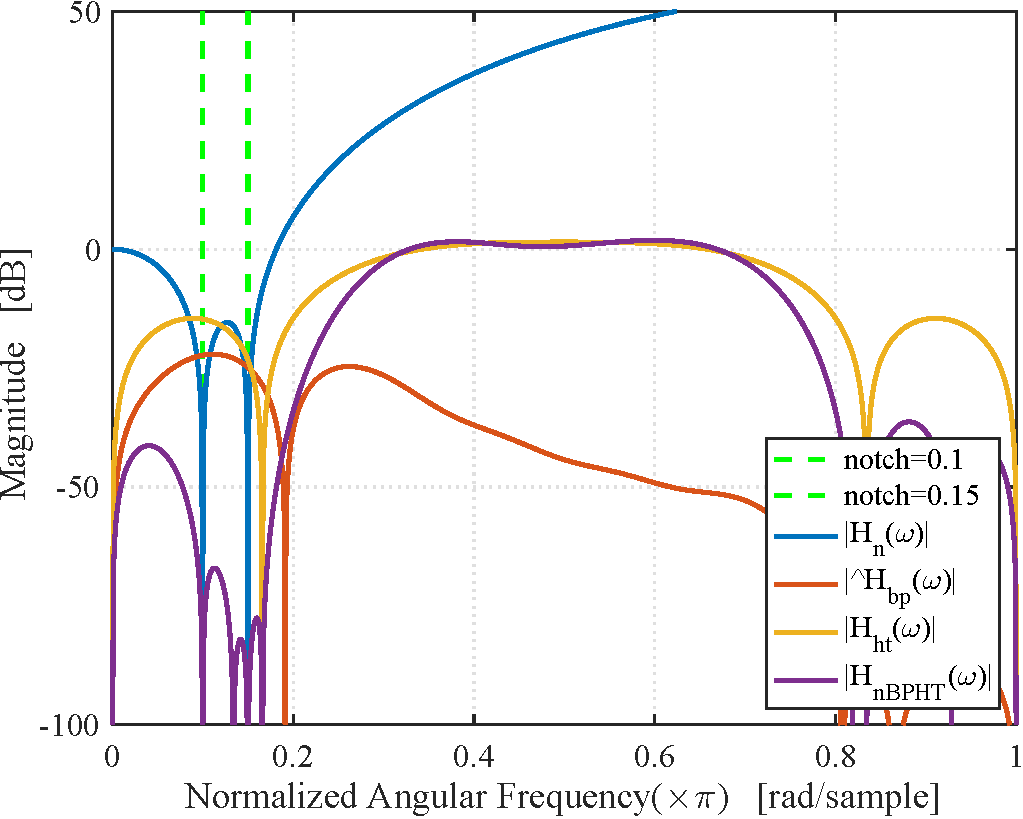
\includegraphics[width=8cm]
    		{Figure/figure01.pdf}
    \caption{のっちだおおおおおおお}
    \label{fig:man}
\end{figure}
%#!platex main.tex
\chapter*{謝辞}
\addcontentsline{toc}{chapter}{謝辞} 
Other/thanks.texで文章を編集して下さい
%本研究にあたり,多大なるご指導とご助
%言を賜わりました.伊丹~ 誠教授,大野~光平先生に深く感謝いたします.また,色々
%な面でご協力いただいた伊丹研究室の大学院生の皆様,卒業研究生に対しまして
%も,心より感謝致します.最後に感謝の意を表して,本論文の謝辞とさせて頂きま
%す.


\include{Other/bibliography}
%#!platex main.tex
\chapter*{発表論文}
\addcontentsline{toc}{chapter}{発表論文}
\def\essection#1{\section*{#1}\addcontentsline{toc}{section}{#1}}

\essection{A.査読あり論文}
\begin{itemize}
\item Other/publicationで編集して下さい
\end{itemize}


\essection{B.国際会議}

\essection{C.研究会}

\essection{D.大会}


\end{document}
\end{verbatim}
のようになっています.

\begin{verbatim}
\documentstyle[12pt,eclepsf,itlbthesis2000,eclclass]{j-report}
\end{verbatim}
でeclclassは\ref{itlbthesis2000ディレクトリ構成}を書くために必要なだけ
です.
ちなみにeclclass.styは\ref{itlbthesis2000ディレクトリ構成}のようなディ
レクトリ構造を書くのに便利なスタイルですが,使わなければ,
\begin{verbatim}
\documentstyle[12pt,eclepsf,itlbthesis2000]{j-report}
\end{verbatim}
としておいて結構です.
12pt.styは文字の大きさを指定するものではずさないでください.
またecleps.styはepsファイルを取り込むものなので,epsファイルを一枚も使わ
ない人ははずしても結構です(たぶんそんなことはない).
更に,スタイルファイル(例えばhere.sty)を追加する場合,
\begin{verbatim}
\documentstyle[12pt,eclepsf,itlbthesis2000,here]{j-report}
\end{verbatim}
のようにすればOKです.

\begin{verbatim}
\begin{document}
\itlbtitle    <---表紙を作ってます
\makeabstract <---アブストラクトを作ってます
\makecontents <---目次を作ってます
\end{verbatim}
は変更しないでください.

\begin{verbatim}
\include{}	
\end{verbatim}
は異なるLaTeXソースをincludeするもので,各章毎に別々のディレクトリで文章を
作ってください.

このようにする理由は次章で述べられているので,次の章は必ず読んでください.

従って,main.texで書き換える必要があるのは
\begin{verbatim}
\include{Introduction/introduction} <--第1章 序論
%#!platex main.tex

\chapter{このスタイルの使い方}
\section{このスタイルファイルについて}
このスタイルファイルの原型は1998年に修士を修了した下村さんが作成したもの
です.
それに初期設定ファイル等を加えて,LaTeXのマクロをブラックボックス化し,
あまりLaTeXのスタイルをわからない人でも使いやすいようにしたつもりです.
本来の目的は,PDF化に際しての編集者の負荷軽減の目的ですが,それほど難し
いスタイルではないので,解析して自分用に書き換えてもらっても結構です.
また,YaTeXを利用する事を前提にして作っている部分もあるので,なじみにく
い人は,過去のスタイルを利用するか,YaTeXを覚えてください.\\
\\
2012.11.20\\
itlbthesis2000.sty(j-tex用)をplatex用に改良したitlbthesis2012.styを作成しました.\\
以下の文章はitlbthesis2000の時のものとなっているので,注意して下さい.
また,バックアップを/home/yakou/Public/Styleの中に保存しておくので,何かありましたら参照してください.
\\
\section{ファイル構成}
まず,

\framebox{\tt gzip -d itlbthesis2000.tar.gz}

とし,

\framebox{\tt tar xvf itlbthesis2000.tar}

とすると,itlbthesis2000というディレクトリができると思います.

\framebox{\tt cd itlbthesis2000}

で中に入ると,その中身は\ref{itlbthesis2000ディレクトリ構成}のようになっ
ています.

ここで,とりあえず,

\framebox{\tt jlatex main.tex}

\framebox{\tt jlatex main.tex}

と2回jlatexをmain.texに対してかけてください.
そこにmain.dviがあるので,

\framebox{\tt xdvi-gs main.dvi}

とすると,このDVIファイルを見ることができます.
\section{設定の方法}
\begin{figure}[htb]
 \begin{center}
  \begin{classify}{\fbox{itlbthesis2000}\hspace*{5cm} $\circ$は全員必須,
   $*$は修士論文のみ必須}
   \class{
   \begin{classify}{\fbox{Introduction}(第1章)}
    \class{introduction.tex(第1章の\LaTeX ソース)}
   \end{classify}
   }
   \class{
   \begin{classify}{\fbox{StyleManual}第2章)}
    \class{stylemanual.tex(第2章の\LaTeX ソース)}
   \end{classify}
   }
   \class{
   \begin{classify}{\fbox{Figure}(第3章)}
    \class{
    \begin{classify}{\fbox{EPS}(第3章用EPSディレクトリ)}
     \class{hogehoge.eps(第3章に関するeps)}
    \end{classify}
    }
    \class{
    \begin{classify}{\fbox{XVD}(第3章用XVDディレクトリ)}
     \class{hogehoge.xvd(第3章に関するxvd)}
    \end{classify}
    }
    \class{figure.tex(第3章の\LaTeX ソース)}
   \end{classify}
   }
   \class{
   \begin{classify}{\fbox{Conclusion}(第4章)}
    \class{conclusion.tex(第4章に関する\LaTeX ソース)}
   \end{classify}
   }
   \class{
   \begin{classify}{\fbox{Other}(その他)}
    \class{abstract.tex(和文アブストラクト$)^{\circ}$}
    \class{abstract\_e.tex(英文アブストラクト$)^{*}$}
    \class{bibliography.tex(参考文献$)^{\circ}$}
    \class{publication.tex(発表論文$)^{*}$}
    \class{thanks.tex(謝辞$)^{\circ}$}
  \end{classify}
   }
   \class{Makefile(メイクファイル$)^{\circ}$}
   \class{eclclass.sty(この絵を書くためのだけのスタイル)}
   \class{init\_thesis.sty(初期設定ファイル$)^{\circ}$}
   \class{itlbthesis2000.sty(メインスタイルファイル$)^{\circ}$}
   \class{main.tex(メイン\LaTeX ソース$)^{\circ}$}
   \class{refcheck.sty(参照チェックスタイル)}
  \end{classify}
 \end{center}
 \caption{itlbthesis2000ディレクトリ構成}
 \label{itlbthesis2000ディレクトリ構成}
\end{figure}
\ref{itlbthesis2000ディレクトリ構成}を見てください.
この中で,itlbthesis2000.styはいじらなくても良いです.
\subsection{init\_thesis.styの書き方}
init\_thesis.styファイルは,初期設定ファイルです.中身は
\begin{verbatim}
%卒業論文の場合   \bm{卒業}
%修士論文の場合   \bm{修士}
\bm{修士}
%伊藤研究室の場合   \lab{伊藤}
%伊丹研究室の場合   \lab{伊丹}
\lab{伊藤}
%西暦の年   \year{}
\year{2001}
%平成の年   \heisei{}
\heisei{12}
%提出する月 \month{}
\month{2}
%論文の和文メインタイトル   \title{}
\title{卒業論文,修士論文の書き方}
%論文の英文メインタイトル(修論のみ)   \titleE{}
%卒論は空欄でOK
\titleE{How to draw up a bachelor's and master's thesis for our laboratory}
%論文の和文サブタイトル   \subtitle{}
%特になければ空欄でもOK 
\subtitle{サブタイトル}
%論文の英文サブタイトル(修論のみ)   \subtitleE{}
%特になければ空欄でもOK
%卒論は空欄でOK
\subtitleE{English sub-title}
%自分の学籍番号   \num{}
\num{8100701}
%自分の日本語の名前   \author{}
\author{藤井 雅弘}
%自分の英語の名前(修論のみ)   \authorE{}
%卒論は空欄でOK
\authorE{Masahiro Fujii}
%和文アブストラクトファイルの指定   \abstract{}
\abstract{Other/abstract.tex}	
%英文アブストラクトファイルの指定(修論のみ)   \abstractE{}
%卒論は空欄でOK
\abstruatE{Other/abstract_e.tex}	
\end{verbatim}
となってきます.
自分で勝手に書き換えてください.

卒論生は''修論のみ''となっている所はそのままでも,空欄でも結構です.
但し,コメントアウトしたり,その行自体を削除したりするとえらいことになり
ます.
一番上の\verb|\bm|を\verb|\bm{卒業}|としておけば,修論のみとなっている所
は反映されません.
\subsection{main.texの書き方}
このmain.dviのTeXソースmain.texは
\begin{verbatim}
\documentstyle[12pt,eclepsf,itlbthesis2000,eclclass]{j-report}
\begin{document}
\itlbtitle
\makeabstract
\makecontents
\include{Introduction/introduction}
\include{StyleManual/stylemanual}
\include{Figure/figure}
\include{Conclusion/conclusion}
\include{Other/thanks}
\include{Other/bibliography}
\include{Other/publication}
\end{document}
\end{verbatim}
のようになっています.

\begin{verbatim}
\documentstyle[12pt,eclepsf,itlbthesis2000,eclclass]{j-report}
\end{verbatim}
でeclclassは\ref{itlbthesis2000ディレクトリ構成}を書くために必要なだけ
です.
ちなみにeclclass.styは\ref{itlbthesis2000ディレクトリ構成}のようなディ
レクトリ構造を書くのに便利なスタイルですが,使わなければ,
\begin{verbatim}
\documentstyle[12pt,eclepsf,itlbthesis2000]{j-report}
\end{verbatim}
としておいて結構です.
12pt.styは文字の大きさを指定するものではずさないでください.
またecleps.styはepsファイルを取り込むものなので,epsファイルを一枚も使わ
ない人ははずしても結構です(たぶんそんなことはない).
更に,スタイルファイル(例えばhere.sty)を追加する場合,
\begin{verbatim}
\documentstyle[12pt,eclepsf,itlbthesis2000,here]{j-report}
\end{verbatim}
のようにすればOKです.

\begin{verbatim}
\begin{document}
\itlbtitle    <---表紙を作ってます
\makeabstract <---アブストラクトを作ってます
\makecontents <---目次を作ってます
\end{verbatim}
は変更しないでください.

\begin{verbatim}
\include{}	
\end{verbatim}
は異なるLaTeXソースをincludeするもので,各章毎に別々のディレクトリで文章を
作ってください.

このようにする理由は次章で述べられているので,次の章は必ず読んでください.

従って,main.texで書き換える必要があるのは
\begin{verbatim}
\include{Introduction/introduction} <--第1章 序論
\include{StyleManual/stylemanual}   <--第2章 スタイルファイルの使い方
\include{Figure/figure}             <--第3章 絵の貼り方
\include{Conclusion/conclusion}     <--第4章 まとめ
\include{Other/thanks}              <--謝辞
\include{Other/publication}         <--発表論文リスト
\include{Other/bibliography}        <--参考文献
\end{verbatim}
です.
\begin{verbatim}
\include{Other/publication}
\end{verbatim}
は発表論文リストファイルですので卒論の場合,\verb|%|でコメントアウトして
 おいてください.

コンパイルの方法は

\framebox{\tt jlatex main.tex}

です.
しかし,これだけだと,目次が構成できないので,もう一度

\framebox{\tt jlatex main.tex}

とやると,目次も構成されます.
ちなみに,

\framebox{\tt make;make final}

とすると,main.psまではきます.
最後の最後の提出の時まではあまり使わないと思います.
修論などで,100ページ以上になると,psファイルがかなりでかくなるので,
 quotaに気をつけてください.
あと

\framebox{\tt make clean}

とすると,ディレクトリ内の掃除ができるのたまにやってもいいかも知れません.

また,yatexを利用すると,圧倒的に効率が良くなります.
この時,各LaTeXファイルに
\begin{verbatim}
%#!jlatex main.tex	
\end{verbatim}
という一行を加えておくと,どのLaTeXファイルからでもmain.texが呼べるので,
現在作業中のLaTeXファイル上で,jlatex main.texができます.
これはかなり便利です.
\section{おまけ}
図や表の引用で\verb|\ref|を利用すると思いますが,このスタイルでは
\verb|\ref{ラベル名}|とすると自動的に{\gt 図 {\bf 1}}のように出力するよ
うになっています.
これは表の引用,本文の引用においても同様です.
これが嫌な人はitlbthesis2012.styの最後の
\begin{verbatim}
\def\p@chapter{{\dg 本文}}
\def\p@section{{\dg 本文}}
\def\p@subsection{{\dg 本文}}
\def\p@subsubsection{{\dg 本文}}
\def\p@figure{{\dg 図}}
\def\p@table{{\dg 表}}
\let\origref=\ref
\def\ref#1{{\bf \origref{#1}}}
\end{verbatim}
を削除してください.


   <--第2章 スタイルファイルの使い方
\include{Figure/figure}             <--第3章 絵の貼り方
%#!platex main.tex
\chapter{序論}

\section{章タイトル}
参考文献のテスト\cite{樋口龍雄2000}.
"bibliography.bib"の中身をいじると変更できます.

あいうえおかきくけこ
正弦波の周波数推定はレーダーやソナー,通信,医療などの領域で幅広く研究されてきた課題である\cite{R.G.McKilliam,K.Wang,D.Rife}.
一般に,単一正弦波に対する周波数推定を行う場合,アナログ信号であれば周波数カウンタを用いる手法,ディジタル信号の場合,相関を用いた手法やヒルベルト変換器を用いる手法が提案されている.
周波数カウンタを用いた手法では,1周期に対して基準クロックを用いて測定し,その逆数から周波数を求めるレシプロカル方式の周波数カウンタが知られている.しかしこの手法を用いる場合,周波数が変化すると出力間隔が不等間隔になる.そのため,計測値に対して,ディジタル処理を行う場合には補完処理などの工夫が必要となるため,サンプルごとに周波数の推定値が出力されるヒルベルト変換器を用いた手法が提案されている.\\
 ヒルベルト変換器を用いた手法では,入力を実部,出力を虚部とする複素信号の一種である解析信号の位相を時間微分し,瞬時角周波数から瞬時周波数を推定することができる.従来,ヒルベルト変換器は有限次数のFIRフィルタとして設計されるため振幅特性にリプルが生じ,出力は振動する場合がある.高尾ら\cite{高尾可変なし,高尾可変あり}は振動成分の周波数が入力周波数の偶数倍であることを理論的に示し,これを伝送零点を有する可変FIRフィルタを用いて振動成分を除去することで,低次数なヒルベルト変換器を用いても,単一正弦波の高精度な瞬時周波数推定が可能となることを示した.
%高尾さんのやつと関連させてノイズを取れることを書きたいなら,どういうノイズが取れて,どういうノイズがダメなのか明記する必要がある.
しかし実際にはノイズを含む信号を解析する必要がある.一般に,ノイズを含む信号に対して,ヒルベルト変換を行うためには,あらかじめ帯域通過フィルタによりノイズを低減させた後に,ヒルベルト変換器を縦続接続する方法が考えられる.しかし,帯域通過フィルタとヒルベルト変換器を1つのフィルタとして見た場合,全体の次数が増加し,結果として遅延や回路規模の増大につながり好ましくない.\\
 そこで本稿では,阻止域を有するヒルベルト変換器に対し,指定した位置に伝送零点を置くことで,ノイズを除去しながらヒルベルト変換可能なフィルタを設計する.阻止域を有するヒルベルト変換器を設計する場合,本来であれば阻止域において十分な減衰量を確保するために多くのフィルタ次数が必要となる.しかし,特定の周波数成分にノイズが含まれることがわかっている場合,その周波数成分のみに伝送零点を入れることにより,特定のノイズのみ除去しながらヒルベルト変換を行うことができ,減衰量を確保するために必要な次数を削減することができる.
最後に設計例を示し,提案法の有効性を確認する.
\section{指定した位置に伝送零点を有するヒルベルト変換器}
本章では提案するフィルタの設計問題について記す.提案するフィルタは,阻止域の指定した位置に伝送零点を有するヒルベルト変換器である.本稿で設計するフィルタの振幅理想特性を図\ref{ideal_resp}に示す.またフィルタの振幅理想特性は正規化角周波数$\omega$を用いて,

\begin{figure}[tb]
    \centering
    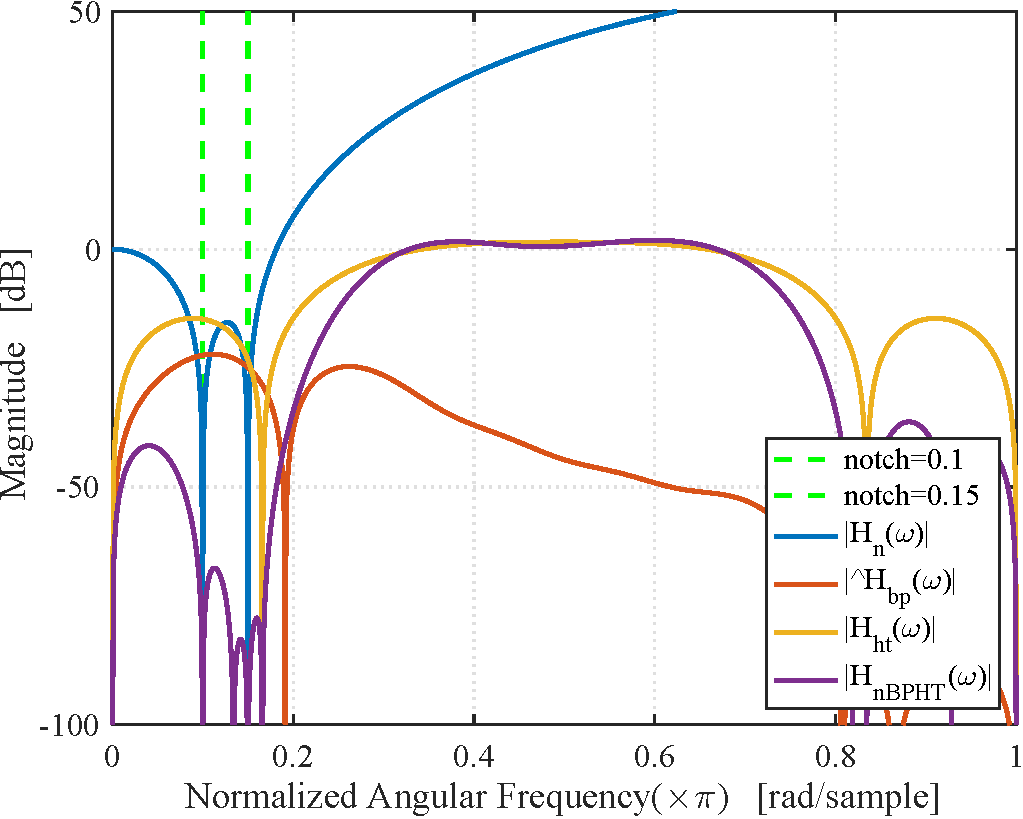
\includegraphics[width=8cm]
    		{Figure/figure01.pdf}
    \caption{のっちだおおおおおおお}
    \label{fig:man}
\end{figure}     <--第4章 まとめ
%#!platex main.tex
\chapter*{謝辞}
\addcontentsline{toc}{chapter}{謝辞} 
Other/thanks.texで文章を編集して下さい
%本研究にあたり,多大なるご指導とご助
%言を賜わりました.伊丹~ 誠教授,大野~光平先生に深く感謝いたします.また,色々
%な面でご協力いただいた伊丹研究室の大学院生の皆様,卒業研究生に対しまして
%も,心より感謝致します.最後に感謝の意を表して,本論文の謝辞とさせて頂きま
%す.

              <--謝辞
%#!platex main.tex
\chapter*{発表論文}
\addcontentsline{toc}{chapter}{発表論文}
\def\essection#1{\section*{#1}\addcontentsline{toc}{section}{#1}}

\essection{A.査読あり論文}
\begin{itemize}
\item Other/publicationで編集して下さい
\end{itemize}


\essection{B.国際会議}

\essection{C.研究会}

\essection{D.大会}

         <--発表論文リスト
\include{Other/bibliography}        <--参考文献
\end{verbatim}
です.
\begin{verbatim}
%#!platex main.tex
\chapter*{発表論文}
\addcontentsline{toc}{chapter}{発表論文}
\def\essection#1{\section*{#1}\addcontentsline{toc}{section}{#1}}

\essection{A.査読あり論文}
\begin{itemize}
\item Other/publicationで編集して下さい
\end{itemize}


\essection{B.国際会議}

\essection{C.研究会}

\essection{D.大会}


\end{verbatim}
は発表論文リストファイルですので卒論の場合,\verb|%|でコメントアウトして
 おいてください.

コンパイルの方法は

\framebox{\tt jlatex main.tex}

です.
しかし,これだけだと,目次が構成できないので,もう一度

\framebox{\tt jlatex main.tex}

とやると,目次も構成されます.
ちなみに,

\framebox{\tt make;make final}

とすると,main.psまではきます.
最後の最後の提出の時まではあまり使わないと思います.
修論などで,100ページ以上になると,psファイルがかなりでかくなるので,
 quotaに気をつけてください.
あと

\framebox{\tt make clean}

とすると,ディレクトリ内の掃除ができるのたまにやってもいいかも知れません.

また,yatexを利用すると,圧倒的に効率が良くなります.
この時,各LaTeXファイルに
\begin{verbatim}
%#!jlatex main.tex	
\end{verbatim}
という一行を加えておくと,どのLaTeXファイルからでもmain.texが呼べるので,
現在作業中のLaTeXファイル上で,jlatex main.texができます.
これはかなり便利です.
\section{おまけ}
図や表の引用で\verb|\ref|を利用すると思いますが,このスタイルでは
\verb|\ref{ラベル名}|とすると自動的に{\gt 図 {\bf 1}}のように出力するよ
うになっています.
これは表の引用,本文の引用においても同様です.
これが嫌な人はitlbthesis2012.styの最後の
\begin{verbatim}
\def\p@chapter{{\dg 本文}}
\def\p@section{{\dg 本文}}
\def\p@subsection{{\dg 本文}}
\def\p@subsubsection{{\dg 本文}}
\def\p@figure{{\dg 図}}
\def\p@table{{\dg 表}}
\let\origref=\ref
\def\ref#1{{\bf \origref{#1}}}
\end{verbatim}
を削除してください.



\include{Figure/figure}
%#!platex main.tex
\chapter{序論}

\section{章タイトル}
参考文献のテスト\cite{樋口龍雄2000}.
"bibliography.bib"の中身をいじると変更できます.

あいうえおかきくけこ
正弦波の周波数推定はレーダーやソナー,通信,医療などの領域で幅広く研究されてきた課題である\cite{R.G.McKilliam,K.Wang,D.Rife}.
一般に,単一正弦波に対する周波数推定を行う場合,アナログ信号であれば周波数カウンタを用いる手法,ディジタル信号の場合,相関を用いた手法やヒルベルト変換器を用いる手法が提案されている.
周波数カウンタを用いた手法では,1周期に対して基準クロックを用いて測定し,その逆数から周波数を求めるレシプロカル方式の周波数カウンタが知られている.しかしこの手法を用いる場合,周波数が変化すると出力間隔が不等間隔になる.そのため,計測値に対して,ディジタル処理を行う場合には補完処理などの工夫が必要となるため,サンプルごとに周波数の推定値が出力されるヒルベルト変換器を用いた手法が提案されている.\\
 ヒルベルト変換器を用いた手法では,入力を実部,出力を虚部とする複素信号の一種である解析信号の位相を時間微分し,瞬時角周波数から瞬時周波数を推定することができる.従来,ヒルベルト変換器は有限次数のFIRフィルタとして設計されるため振幅特性にリプルが生じ,出力は振動する場合がある.高尾ら\cite{高尾可変なし,高尾可変あり}は振動成分の周波数が入力周波数の偶数倍であることを理論的に示し,これを伝送零点を有する可変FIRフィルタを用いて振動成分を除去することで,低次数なヒルベルト変換器を用いても,単一正弦波の高精度な瞬時周波数推定が可能となることを示した.
%高尾さんのやつと関連させてノイズを取れることを書きたいなら,どういうノイズが取れて,どういうノイズがダメなのか明記する必要がある.
しかし実際にはノイズを含む信号を解析する必要がある.一般に,ノイズを含む信号に対して,ヒルベルト変換を行うためには,あらかじめ帯域通過フィルタによりノイズを低減させた後に,ヒルベルト変換器を縦続接続する方法が考えられる.しかし,帯域通過フィルタとヒルベルト変換器を1つのフィルタとして見た場合,全体の次数が増加し,結果として遅延や回路規模の増大につながり好ましくない.\\
 そこで本稿では,阻止域を有するヒルベルト変換器に対し,指定した位置に伝送零点を置くことで,ノイズを除去しながらヒルベルト変換可能なフィルタを設計する.阻止域を有するヒルベルト変換器を設計する場合,本来であれば阻止域において十分な減衰量を確保するために多くのフィルタ次数が必要となる.しかし,特定の周波数成分にノイズが含まれることがわかっている場合,その周波数成分のみに伝送零点を入れることにより,特定のノイズのみ除去しながらヒルベルト変換を行うことができ,減衰量を確保するために必要な次数を削減することができる.
最後に設計例を示し,提案法の有効性を確認する.
\section{指定した位置に伝送零点を有するヒルベルト変換器}
本章では提案するフィルタの設計問題について記す.提案するフィルタは,阻止域の指定した位置に伝送零点を有するヒルベルト変換器である.本稿で設計するフィルタの振幅理想特性を図\ref{ideal_resp}に示す.またフィルタの振幅理想特性は正規化角周波数$\omega$を用いて,

\begin{figure}[tb]
    \centering
    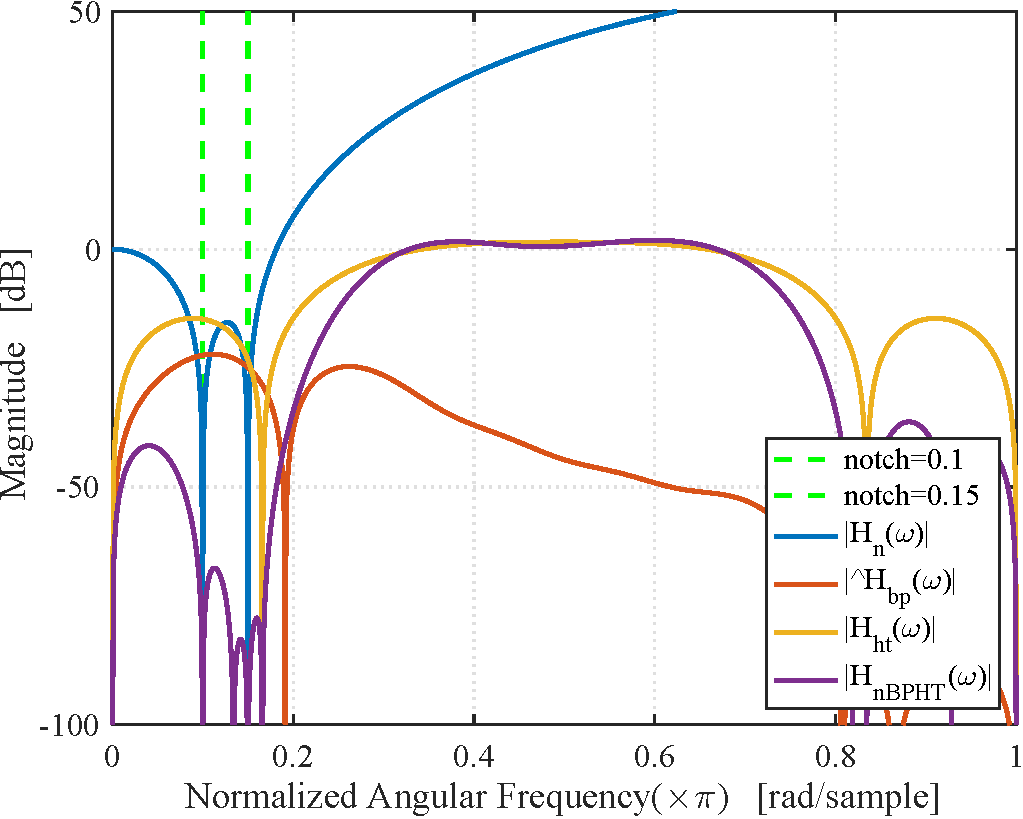
\includegraphics[width=8cm]
    		{Figure/figure01.pdf}
    \caption{のっちだおおおおおおお}
    \label{fig:man}
\end{figure}
%#!platex main.tex
\chapter*{謝辞}
\addcontentsline{toc}{chapter}{謝辞} 
Other/thanks.texで文章を編集して下さい
%本研究にあたり,多大なるご指導とご助
%言を賜わりました.伊丹~ 誠教授,大野~光平先生に深く感謝いたします.また,色々
%な面でご協力いただいた伊丹研究室の大学院生の皆様,卒業研究生に対しまして
%も,心より感謝致します.最後に感謝の意を表して,本論文の謝辞とさせて頂きま
%す.


\include{Other/bibliography}
%#!platex main.tex
\chapter*{発表論文}
\addcontentsline{toc}{chapter}{発表論文}
\def\essection#1{\section*{#1}\addcontentsline{toc}{section}{#1}}

\essection{A.査読あり論文}
\begin{itemize}
\item Other/publicationで編集して下さい
\end{itemize}


\essection{B.国際会議}

\essection{C.研究会}

\essection{D.大会}


\end{document}
\end{verbatim}
のようになっています.

\begin{verbatim}
\documentstyle[12pt,eclepsf,itlbthesis2000,eclclass]{j-report}
\end{verbatim}
でeclclassは\ref{itlbthesis2000ディレクトリ構成}を書くために必要なだけ
です.
ちなみにeclclass.styは\ref{itlbthesis2000ディレクトリ構成}のようなディ
レクトリ構造を書くのに便利なスタイルですが,使わなければ,
\begin{verbatim}
\documentstyle[12pt,eclepsf,itlbthesis2000]{j-report}
\end{verbatim}
としておいて結構です.
12pt.styは文字の大きさを指定するものではずさないでください.
またecleps.styはepsファイルを取り込むものなので,epsファイルを一枚も使わ
ない人ははずしても結構です(たぶんそんなことはない).
更に,スタイルファイル(例えばhere.sty)を追加する場合,
\begin{verbatim}
\documentstyle[12pt,eclepsf,itlbthesis2000,here]{j-report}
\end{verbatim}
のようにすればOKです.

\begin{verbatim}
\begin{document}
\itlbtitle    <---表紙を作ってます
\makeabstract <---アブストラクトを作ってます
\makecontents <---目次を作ってます
\end{verbatim}
は変更しないでください.

\begin{verbatim}
\include{}	
\end{verbatim}
は異なるLaTeXソースをincludeするもので,各章毎に別々のディレクトリで文章を
作ってください.

このようにする理由は次章で述べられているので,次の章は必ず読んでください.

従って,main.texで書き換える必要があるのは
\begin{verbatim}
\include{Introduction/introduction} <--第1章 序論
%#!platex main.tex

\chapter{このスタイルの使い方}
\section{このスタイルファイルについて}
このスタイルファイルの原型は1998年に修士を修了した下村さんが作成したもの
です.
それに初期設定ファイル等を加えて,LaTeXのマクロをブラックボックス化し,
あまりLaTeXのスタイルをわからない人でも使いやすいようにしたつもりです.
本来の目的は,PDF化に際しての編集者の負荷軽減の目的ですが,それほど難し
いスタイルではないので,解析して自分用に書き換えてもらっても結構です.
また,YaTeXを利用する事を前提にして作っている部分もあるので,なじみにく
い人は,過去のスタイルを利用するか,YaTeXを覚えてください.\\
\\
2012.11.20\\
itlbthesis2000.sty(j-tex用)をplatex用に改良したitlbthesis2012.styを作成しました.\\
以下の文章はitlbthesis2000の時のものとなっているので,注意して下さい.
また,バックアップを/home/yakou/Public/Styleの中に保存しておくので,何かありましたら参照してください.
\\
\section{ファイル構成}
まず,

\framebox{\tt gzip -d itlbthesis2000.tar.gz}

とし,

\framebox{\tt tar xvf itlbthesis2000.tar}

とすると,itlbthesis2000というディレクトリができると思います.

\framebox{\tt cd itlbthesis2000}

で中に入ると,その中身は\ref{itlbthesis2000ディレクトリ構成}のようになっ
ています.

ここで,とりあえず,

\framebox{\tt jlatex main.tex}

\framebox{\tt jlatex main.tex}

と2回jlatexをmain.texに対してかけてください.
そこにmain.dviがあるので,

\framebox{\tt xdvi-gs main.dvi}

とすると,このDVIファイルを見ることができます.
\section{設定の方法}
\begin{figure}[htb]
 \begin{center}
  \begin{classify}{\fbox{itlbthesis2000}\hspace*{5cm} $\circ$は全員必須,
   $*$は修士論文のみ必須}
   \class{
   \begin{classify}{\fbox{Introduction}(第1章)}
    \class{introduction.tex(第1章の\LaTeX ソース)}
   \end{classify}
   }
   \class{
   \begin{classify}{\fbox{StyleManual}第2章)}
    \class{stylemanual.tex(第2章の\LaTeX ソース)}
   \end{classify}
   }
   \class{
   \begin{classify}{\fbox{Figure}(第3章)}
    \class{
    \begin{classify}{\fbox{EPS}(第3章用EPSディレクトリ)}
     \class{hogehoge.eps(第3章に関するeps)}
    \end{classify}
    }
    \class{
    \begin{classify}{\fbox{XVD}(第3章用XVDディレクトリ)}
     \class{hogehoge.xvd(第3章に関するxvd)}
    \end{classify}
    }
    \class{figure.tex(第3章の\LaTeX ソース)}
   \end{classify}
   }
   \class{
   \begin{classify}{\fbox{Conclusion}(第4章)}
    \class{conclusion.tex(第4章に関する\LaTeX ソース)}
   \end{classify}
   }
   \class{
   \begin{classify}{\fbox{Other}(その他)}
    \class{abstract.tex(和文アブストラクト$)^{\circ}$}
    \class{abstract\_e.tex(英文アブストラクト$)^{*}$}
    \class{bibliography.tex(参考文献$)^{\circ}$}
    \class{publication.tex(発表論文$)^{*}$}
    \class{thanks.tex(謝辞$)^{\circ}$}
  \end{classify}
   }
   \class{Makefile(メイクファイル$)^{\circ}$}
   \class{eclclass.sty(この絵を書くためのだけのスタイル)}
   \class{init\_thesis.sty(初期設定ファイル$)^{\circ}$}
   \class{itlbthesis2000.sty(メインスタイルファイル$)^{\circ}$}
   \class{main.tex(メイン\LaTeX ソース$)^{\circ}$}
   \class{refcheck.sty(参照チェックスタイル)}
  \end{classify}
 \end{center}
 \caption{itlbthesis2000ディレクトリ構成}
 \label{itlbthesis2000ディレクトリ構成}
\end{figure}
\ref{itlbthesis2000ディレクトリ構成}を見てください.
この中で,itlbthesis2000.styはいじらなくても良いです.
\subsection{init\_thesis.styの書き方}
init\_thesis.styファイルは,初期設定ファイルです.中身は
\begin{verbatim}
%卒業論文の場合   \bm{卒業}
%修士論文の場合   \bm{修士}
\bm{修士}
%伊藤研究室の場合   \lab{伊藤}
%伊丹研究室の場合   \lab{伊丹}
\lab{伊藤}
%西暦の年   \year{}
\year{2001}
%平成の年   \heisei{}
\heisei{12}
%提出する月 \month{}
\month{2}
%論文の和文メインタイトル   \title{}
\title{卒業論文,修士論文の書き方}
%論文の英文メインタイトル(修論のみ)   \titleE{}
%卒論は空欄でOK
\titleE{How to draw up a bachelor's and master's thesis for our laboratory}
%論文の和文サブタイトル   \subtitle{}
%特になければ空欄でもOK 
\subtitle{サブタイトル}
%論文の英文サブタイトル(修論のみ)   \subtitleE{}
%特になければ空欄でもOK
%卒論は空欄でOK
\subtitleE{English sub-title}
%自分の学籍番号   \num{}
\num{8100701}
%自分の日本語の名前   \author{}
\author{藤井 雅弘}
%自分の英語の名前(修論のみ)   \authorE{}
%卒論は空欄でOK
\authorE{Masahiro Fujii}
%和文アブストラクトファイルの指定   \abstract{}
\abstract{Other/abstract.tex}	
%英文アブストラクトファイルの指定(修論のみ)   \abstractE{}
%卒論は空欄でOK
\abstruatE{Other/abstract_e.tex}	
\end{verbatim}
となってきます.
自分で勝手に書き換えてください.

卒論生は''修論のみ''となっている所はそのままでも,空欄でも結構です.
但し,コメントアウトしたり,その行自体を削除したりするとえらいことになり
ます.
一番上の\verb|\bm|を\verb|\bm{卒業}|としておけば,修論のみとなっている所
は反映されません.
\subsection{main.texの書き方}
このmain.dviのTeXソースmain.texは
\begin{verbatim}
\documentstyle[12pt,eclepsf,itlbthesis2000,eclclass]{j-report}
\begin{document}
\itlbtitle
\makeabstract
\makecontents
\include{Introduction/introduction}
%#!platex main.tex

\chapter{このスタイルの使い方}
\section{このスタイルファイルについて}
このスタイルファイルの原型は1998年に修士を修了した下村さんが作成したもの
です.
それに初期設定ファイル等を加えて,LaTeXのマクロをブラックボックス化し,
あまりLaTeXのスタイルをわからない人でも使いやすいようにしたつもりです.
本来の目的は,PDF化に際しての編集者の負荷軽減の目的ですが,それほど難し
いスタイルではないので,解析して自分用に書き換えてもらっても結構です.
また,YaTeXを利用する事を前提にして作っている部分もあるので,なじみにく
い人は,過去のスタイルを利用するか,YaTeXを覚えてください.\\
\\
2012.11.20\\
itlbthesis2000.sty(j-tex用)をplatex用に改良したitlbthesis2012.styを作成しました.\\
以下の文章はitlbthesis2000の時のものとなっているので,注意して下さい.
また,バックアップを/home/yakou/Public/Styleの中に保存しておくので,何かありましたら参照してください.
\\
\section{ファイル構成}
まず,

\framebox{\tt gzip -d itlbthesis2000.tar.gz}

とし,

\framebox{\tt tar xvf itlbthesis2000.tar}

とすると,itlbthesis2000というディレクトリができると思います.

\framebox{\tt cd itlbthesis2000}

で中に入ると,その中身は\ref{itlbthesis2000ディレクトリ構成}のようになっ
ています.

ここで,とりあえず,

\framebox{\tt jlatex main.tex}

\framebox{\tt jlatex main.tex}

と2回jlatexをmain.texに対してかけてください.
そこにmain.dviがあるので,

\framebox{\tt xdvi-gs main.dvi}

とすると,このDVIファイルを見ることができます.
\section{設定の方法}
\begin{figure}[htb]
 \begin{center}
  \begin{classify}{\fbox{itlbthesis2000}\hspace*{5cm} $\circ$は全員必須,
   $*$は修士論文のみ必須}
   \class{
   \begin{classify}{\fbox{Introduction}(第1章)}
    \class{introduction.tex(第1章の\LaTeX ソース)}
   \end{classify}
   }
   \class{
   \begin{classify}{\fbox{StyleManual}第2章)}
    \class{stylemanual.tex(第2章の\LaTeX ソース)}
   \end{classify}
   }
   \class{
   \begin{classify}{\fbox{Figure}(第3章)}
    \class{
    \begin{classify}{\fbox{EPS}(第3章用EPSディレクトリ)}
     \class{hogehoge.eps(第3章に関するeps)}
    \end{classify}
    }
    \class{
    \begin{classify}{\fbox{XVD}(第3章用XVDディレクトリ)}
     \class{hogehoge.xvd(第3章に関するxvd)}
    \end{classify}
    }
    \class{figure.tex(第3章の\LaTeX ソース)}
   \end{classify}
   }
   \class{
   \begin{classify}{\fbox{Conclusion}(第4章)}
    \class{conclusion.tex(第4章に関する\LaTeX ソース)}
   \end{classify}
   }
   \class{
   \begin{classify}{\fbox{Other}(その他)}
    \class{abstract.tex(和文アブストラクト$)^{\circ}$}
    \class{abstract\_e.tex(英文アブストラクト$)^{*}$}
    \class{bibliography.tex(参考文献$)^{\circ}$}
    \class{publication.tex(発表論文$)^{*}$}
    \class{thanks.tex(謝辞$)^{\circ}$}
  \end{classify}
   }
   \class{Makefile(メイクファイル$)^{\circ}$}
   \class{eclclass.sty(この絵を書くためのだけのスタイル)}
   \class{init\_thesis.sty(初期設定ファイル$)^{\circ}$}
   \class{itlbthesis2000.sty(メインスタイルファイル$)^{\circ}$}
   \class{main.tex(メイン\LaTeX ソース$)^{\circ}$}
   \class{refcheck.sty(参照チェックスタイル)}
  \end{classify}
 \end{center}
 \caption{itlbthesis2000ディレクトリ構成}
 \label{itlbthesis2000ディレクトリ構成}
\end{figure}
\ref{itlbthesis2000ディレクトリ構成}を見てください.
この中で,itlbthesis2000.styはいじらなくても良いです.
\subsection{init\_thesis.styの書き方}
init\_thesis.styファイルは,初期設定ファイルです.中身は
\begin{verbatim}
%卒業論文の場合   \bm{卒業}
%修士論文の場合   \bm{修士}
\bm{修士}
%伊藤研究室の場合   \lab{伊藤}
%伊丹研究室の場合   \lab{伊丹}
\lab{伊藤}
%西暦の年   \year{}
\year{2001}
%平成の年   \heisei{}
\heisei{12}
%提出する月 \month{}
\month{2}
%論文の和文メインタイトル   \title{}
\title{卒業論文,修士論文の書き方}
%論文の英文メインタイトル(修論のみ)   \titleE{}
%卒論は空欄でOK
\titleE{How to draw up a bachelor's and master's thesis for our laboratory}
%論文の和文サブタイトル   \subtitle{}
%特になければ空欄でもOK 
\subtitle{サブタイトル}
%論文の英文サブタイトル(修論のみ)   \subtitleE{}
%特になければ空欄でもOK
%卒論は空欄でOK
\subtitleE{English sub-title}
%自分の学籍番号   \num{}
\num{8100701}
%自分の日本語の名前   \author{}
\author{藤井 雅弘}
%自分の英語の名前(修論のみ)   \authorE{}
%卒論は空欄でOK
\authorE{Masahiro Fujii}
%和文アブストラクトファイルの指定   \abstract{}
\abstract{Other/abstract.tex}	
%英文アブストラクトファイルの指定(修論のみ)   \abstractE{}
%卒論は空欄でOK
\abstruatE{Other/abstract_e.tex}	
\end{verbatim}
となってきます.
自分で勝手に書き換えてください.

卒論生は''修論のみ''となっている所はそのままでも,空欄でも結構です.
但し,コメントアウトしたり,その行自体を削除したりするとえらいことになり
ます.
一番上の\verb|\bm|を\verb|\bm{卒業}|としておけば,修論のみとなっている所
は反映されません.
\subsection{main.texの書き方}
このmain.dviのTeXソースmain.texは
\begin{verbatim}
\documentstyle[12pt,eclepsf,itlbthesis2000,eclclass]{j-report}
\begin{document}
\itlbtitle
\makeabstract
\makecontents
\include{Introduction/introduction}
\include{StyleManual/stylemanual}
\include{Figure/figure}
\include{Conclusion/conclusion}
\include{Other/thanks}
\include{Other/bibliography}
\include{Other/publication}
\end{document}
\end{verbatim}
のようになっています.

\begin{verbatim}
\documentstyle[12pt,eclepsf,itlbthesis2000,eclclass]{j-report}
\end{verbatim}
でeclclassは\ref{itlbthesis2000ディレクトリ構成}を書くために必要なだけ
です.
ちなみにeclclass.styは\ref{itlbthesis2000ディレクトリ構成}のようなディ
レクトリ構造を書くのに便利なスタイルですが,使わなければ,
\begin{verbatim}
\documentstyle[12pt,eclepsf,itlbthesis2000]{j-report}
\end{verbatim}
としておいて結構です.
12pt.styは文字の大きさを指定するものではずさないでください.
またecleps.styはepsファイルを取り込むものなので,epsファイルを一枚も使わ
ない人ははずしても結構です(たぶんそんなことはない).
更に,スタイルファイル(例えばhere.sty)を追加する場合,
\begin{verbatim}
\documentstyle[12pt,eclepsf,itlbthesis2000,here]{j-report}
\end{verbatim}
のようにすればOKです.

\begin{verbatim}
\begin{document}
\itlbtitle    <---表紙を作ってます
\makeabstract <---アブストラクトを作ってます
\makecontents <---目次を作ってます
\end{verbatim}
は変更しないでください.

\begin{verbatim}
\include{}	
\end{verbatim}
は異なるLaTeXソースをincludeするもので,各章毎に別々のディレクトリで文章を
作ってください.

このようにする理由は次章で述べられているので,次の章は必ず読んでください.

従って,main.texで書き換える必要があるのは
\begin{verbatim}
\include{Introduction/introduction} <--第1章 序論
\include{StyleManual/stylemanual}   <--第2章 スタイルファイルの使い方
\include{Figure/figure}             <--第3章 絵の貼り方
\include{Conclusion/conclusion}     <--第4章 まとめ
\include{Other/thanks}              <--謝辞
\include{Other/publication}         <--発表論文リスト
\include{Other/bibliography}        <--参考文献
\end{verbatim}
です.
\begin{verbatim}
\include{Other/publication}
\end{verbatim}
は発表論文リストファイルですので卒論の場合,\verb|%|でコメントアウトして
 おいてください.

コンパイルの方法は

\framebox{\tt jlatex main.tex}

です.
しかし,これだけだと,目次が構成できないので,もう一度

\framebox{\tt jlatex main.tex}

とやると,目次も構成されます.
ちなみに,

\framebox{\tt make;make final}

とすると,main.psまではきます.
最後の最後の提出の時まではあまり使わないと思います.
修論などで,100ページ以上になると,psファイルがかなりでかくなるので,
 quotaに気をつけてください.
あと

\framebox{\tt make clean}

とすると,ディレクトリ内の掃除ができるのたまにやってもいいかも知れません.

また,yatexを利用すると,圧倒的に効率が良くなります.
この時,各LaTeXファイルに
\begin{verbatim}
%#!jlatex main.tex	
\end{verbatim}
という一行を加えておくと,どのLaTeXファイルからでもmain.texが呼べるので,
現在作業中のLaTeXファイル上で,jlatex main.texができます.
これはかなり便利です.
\section{おまけ}
図や表の引用で\verb|\ref|を利用すると思いますが,このスタイルでは
\verb|\ref{ラベル名}|とすると自動的に{\gt 図 {\bf 1}}のように出力するよ
うになっています.
これは表の引用,本文の引用においても同様です.
これが嫌な人はitlbthesis2012.styの最後の
\begin{verbatim}
\def\p@chapter{{\dg 本文}}
\def\p@section{{\dg 本文}}
\def\p@subsection{{\dg 本文}}
\def\p@subsubsection{{\dg 本文}}
\def\p@figure{{\dg 図}}
\def\p@table{{\dg 表}}
\let\origref=\ref
\def\ref#1{{\bf \origref{#1}}}
\end{verbatim}
を削除してください.



\include{Figure/figure}
%#!platex main.tex
\chapter{序論}

\section{章タイトル}
参考文献のテスト\cite{樋口龍雄2000}.
"bibliography.bib"の中身をいじると変更できます.

あいうえおかきくけこ
正弦波の周波数推定はレーダーやソナー,通信,医療などの領域で幅広く研究されてきた課題である\cite{R.G.McKilliam,K.Wang,D.Rife}.
一般に,単一正弦波に対する周波数推定を行う場合,アナログ信号であれば周波数カウンタを用いる手法,ディジタル信号の場合,相関を用いた手法やヒルベルト変換器を用いる手法が提案されている.
周波数カウンタを用いた手法では,1周期に対して基準クロックを用いて測定し,その逆数から周波数を求めるレシプロカル方式の周波数カウンタが知られている.しかしこの手法を用いる場合,周波数が変化すると出力間隔が不等間隔になる.そのため,計測値に対して,ディジタル処理を行う場合には補完処理などの工夫が必要となるため,サンプルごとに周波数の推定値が出力されるヒルベルト変換器を用いた手法が提案されている.\\
 ヒルベルト変換器を用いた手法では,入力を実部,出力を虚部とする複素信号の一種である解析信号の位相を時間微分し,瞬時角周波数から瞬時周波数を推定することができる.従来,ヒルベルト変換器は有限次数のFIRフィルタとして設計されるため振幅特性にリプルが生じ,出力は振動する場合がある.高尾ら\cite{高尾可変なし,高尾可変あり}は振動成分の周波数が入力周波数の偶数倍であることを理論的に示し,これを伝送零点を有する可変FIRフィルタを用いて振動成分を除去することで,低次数なヒルベルト変換器を用いても,単一正弦波の高精度な瞬時周波数推定が可能となることを示した.
%高尾さんのやつと関連させてノイズを取れることを書きたいなら,どういうノイズが取れて,どういうノイズがダメなのか明記する必要がある.
しかし実際にはノイズを含む信号を解析する必要がある.一般に,ノイズを含む信号に対して,ヒルベルト変換を行うためには,あらかじめ帯域通過フィルタによりノイズを低減させた後に,ヒルベルト変換器を縦続接続する方法が考えられる.しかし,帯域通過フィルタとヒルベルト変換器を1つのフィルタとして見た場合,全体の次数が増加し,結果として遅延や回路規模の増大につながり好ましくない.\\
 そこで本稿では,阻止域を有するヒルベルト変換器に対し,指定した位置に伝送零点を置くことで,ノイズを除去しながらヒルベルト変換可能なフィルタを設計する.阻止域を有するヒルベルト変換器を設計する場合,本来であれば阻止域において十分な減衰量を確保するために多くのフィルタ次数が必要となる.しかし,特定の周波数成分にノイズが含まれることがわかっている場合,その周波数成分のみに伝送零点を入れることにより,特定のノイズのみ除去しながらヒルベルト変換を行うことができ,減衰量を確保するために必要な次数を削減することができる.
最後に設計例を示し,提案法の有効性を確認する.
\section{指定した位置に伝送零点を有するヒルベルト変換器}
本章では提案するフィルタの設計問題について記す.提案するフィルタは,阻止域の指定した位置に伝送零点を有するヒルベルト変換器である.本稿で設計するフィルタの振幅理想特性を図\ref{ideal_resp}に示す.またフィルタの振幅理想特性は正規化角周波数$\omega$を用いて,

\begin{figure}[tb]
    \centering
    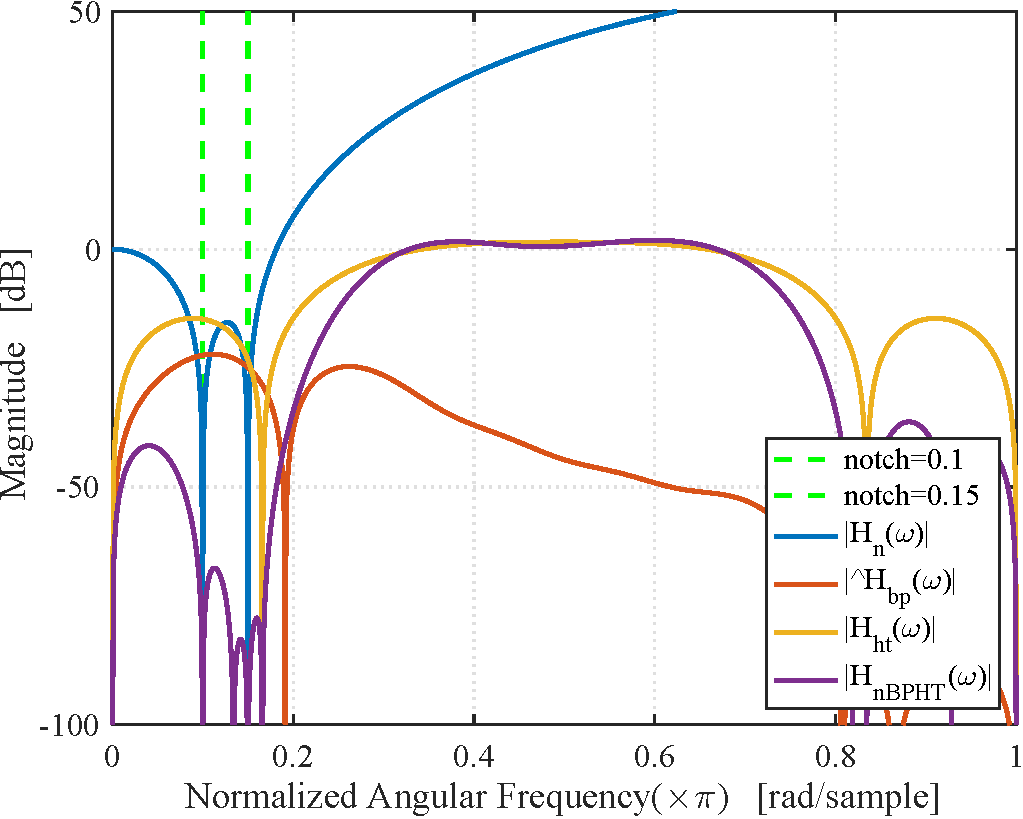
\includegraphics[width=8cm]
    		{Figure/figure01.pdf}
    \caption{のっちだおおおおおおお}
    \label{fig:man}
\end{figure}
%#!platex main.tex
\chapter*{謝辞}
\addcontentsline{toc}{chapter}{謝辞} 
Other/thanks.texで文章を編集して下さい
%本研究にあたり,多大なるご指導とご助
%言を賜わりました.伊丹~ 誠教授,大野~光平先生に深く感謝いたします.また,色々
%な面でご協力いただいた伊丹研究室の大学院生の皆様,卒業研究生に対しまして
%も,心より感謝致します.最後に感謝の意を表して,本論文の謝辞とさせて頂きま
%す.


\include{Other/bibliography}
%#!platex main.tex
\chapter*{発表論文}
\addcontentsline{toc}{chapter}{発表論文}
\def\essection#1{\section*{#1}\addcontentsline{toc}{section}{#1}}

\essection{A.査読あり論文}
\begin{itemize}
\item Other/publicationで編集して下さい
\end{itemize}


\essection{B.国際会議}

\essection{C.研究会}

\essection{D.大会}


\end{document}
\end{verbatim}
のようになっています.

\begin{verbatim}
\documentstyle[12pt,eclepsf,itlbthesis2000,eclclass]{j-report}
\end{verbatim}
でeclclassは\ref{itlbthesis2000ディレクトリ構成}を書くために必要なだけ
です.
ちなみにeclclass.styは\ref{itlbthesis2000ディレクトリ構成}のようなディ
レクトリ構造を書くのに便利なスタイルですが,使わなければ,
\begin{verbatim}
\documentstyle[12pt,eclepsf,itlbthesis2000]{j-report}
\end{verbatim}
としておいて結構です.
12pt.styは文字の大きさを指定するものではずさないでください.
またecleps.styはepsファイルを取り込むものなので,epsファイルを一枚も使わ
ない人ははずしても結構です(たぶんそんなことはない).
更に,スタイルファイル(例えばhere.sty)を追加する場合,
\begin{verbatim}
\documentstyle[12pt,eclepsf,itlbthesis2000,here]{j-report}
\end{verbatim}
のようにすればOKです.

\begin{verbatim}
\begin{document}
\itlbtitle    <---表紙を作ってます
\makeabstract <---アブストラクトを作ってます
\makecontents <---目次を作ってます
\end{verbatim}
は変更しないでください.

\begin{verbatim}
\include{}	
\end{verbatim}
は異なるLaTeXソースをincludeするもので,各章毎に別々のディレクトリで文章を
作ってください.

このようにする理由は次章で述べられているので,次の章は必ず読んでください.

従って,main.texで書き換える必要があるのは
\begin{verbatim}
\include{Introduction/introduction} <--第1章 序論
%#!platex main.tex

\chapter{このスタイルの使い方}
\section{このスタイルファイルについて}
このスタイルファイルの原型は1998年に修士を修了した下村さんが作成したもの
です.
それに初期設定ファイル等を加えて,LaTeXのマクロをブラックボックス化し,
あまりLaTeXのスタイルをわからない人でも使いやすいようにしたつもりです.
本来の目的は,PDF化に際しての編集者の負荷軽減の目的ですが,それほど難し
いスタイルではないので,解析して自分用に書き換えてもらっても結構です.
また,YaTeXを利用する事を前提にして作っている部分もあるので,なじみにく
い人は,過去のスタイルを利用するか,YaTeXを覚えてください.\\
\\
2012.11.20\\
itlbthesis2000.sty(j-tex用)をplatex用に改良したitlbthesis2012.styを作成しました.\\
以下の文章はitlbthesis2000の時のものとなっているので,注意して下さい.
また,バックアップを/home/yakou/Public/Styleの中に保存しておくので,何かありましたら参照してください.
\\
\section{ファイル構成}
まず,

\framebox{\tt gzip -d itlbthesis2000.tar.gz}

とし,

\framebox{\tt tar xvf itlbthesis2000.tar}

とすると,itlbthesis2000というディレクトリができると思います.

\framebox{\tt cd itlbthesis2000}

で中に入ると,その中身は\ref{itlbthesis2000ディレクトリ構成}のようになっ
ています.

ここで,とりあえず,

\framebox{\tt jlatex main.tex}

\framebox{\tt jlatex main.tex}

と2回jlatexをmain.texに対してかけてください.
そこにmain.dviがあるので,

\framebox{\tt xdvi-gs main.dvi}

とすると,このDVIファイルを見ることができます.
\section{設定の方法}
\begin{figure}[htb]
 \begin{center}
  \begin{classify}{\fbox{itlbthesis2000}\hspace*{5cm} $\circ$は全員必須,
   $*$は修士論文のみ必須}
   \class{
   \begin{classify}{\fbox{Introduction}(第1章)}
    \class{introduction.tex(第1章の\LaTeX ソース)}
   \end{classify}
   }
   \class{
   \begin{classify}{\fbox{StyleManual}第2章)}
    \class{stylemanual.tex(第2章の\LaTeX ソース)}
   \end{classify}
   }
   \class{
   \begin{classify}{\fbox{Figure}(第3章)}
    \class{
    \begin{classify}{\fbox{EPS}(第3章用EPSディレクトリ)}
     \class{hogehoge.eps(第3章に関するeps)}
    \end{classify}
    }
    \class{
    \begin{classify}{\fbox{XVD}(第3章用XVDディレクトリ)}
     \class{hogehoge.xvd(第3章に関するxvd)}
    \end{classify}
    }
    \class{figure.tex(第3章の\LaTeX ソース)}
   \end{classify}
   }
   \class{
   \begin{classify}{\fbox{Conclusion}(第4章)}
    \class{conclusion.tex(第4章に関する\LaTeX ソース)}
   \end{classify}
   }
   \class{
   \begin{classify}{\fbox{Other}(その他)}
    \class{abstract.tex(和文アブストラクト$)^{\circ}$}
    \class{abstract\_e.tex(英文アブストラクト$)^{*}$}
    \class{bibliography.tex(参考文献$)^{\circ}$}
    \class{publication.tex(発表論文$)^{*}$}
    \class{thanks.tex(謝辞$)^{\circ}$}
  \end{classify}
   }
   \class{Makefile(メイクファイル$)^{\circ}$}
   \class{eclclass.sty(この絵を書くためのだけのスタイル)}
   \class{init\_thesis.sty(初期設定ファイル$)^{\circ}$}
   \class{itlbthesis2000.sty(メインスタイルファイル$)^{\circ}$}
   \class{main.tex(メイン\LaTeX ソース$)^{\circ}$}
   \class{refcheck.sty(参照チェックスタイル)}
  \end{classify}
 \end{center}
 \caption{itlbthesis2000ディレクトリ構成}
 \label{itlbthesis2000ディレクトリ構成}
\end{figure}
\ref{itlbthesis2000ディレクトリ構成}を見てください.
この中で,itlbthesis2000.styはいじらなくても良いです.
\subsection{init\_thesis.styの書き方}
init\_thesis.styファイルは,初期設定ファイルです.中身は
\begin{verbatim}
%卒業論文の場合   \bm{卒業}
%修士論文の場合   \bm{修士}
\bm{修士}
%伊藤研究室の場合   \lab{伊藤}
%伊丹研究室の場合   \lab{伊丹}
\lab{伊藤}
%西暦の年   \year{}
\year{2001}
%平成の年   \heisei{}
\heisei{12}
%提出する月 \month{}
\month{2}
%論文の和文メインタイトル   \title{}
\title{卒業論文,修士論文の書き方}
%論文の英文メインタイトル(修論のみ)   \titleE{}
%卒論は空欄でOK
\titleE{How to draw up a bachelor's and master's thesis for our laboratory}
%論文の和文サブタイトル   \subtitle{}
%特になければ空欄でもOK 
\subtitle{サブタイトル}
%論文の英文サブタイトル(修論のみ)   \subtitleE{}
%特になければ空欄でもOK
%卒論は空欄でOK
\subtitleE{English sub-title}
%自分の学籍番号   \num{}
\num{8100701}
%自分の日本語の名前   \author{}
\author{藤井 雅弘}
%自分の英語の名前(修論のみ)   \authorE{}
%卒論は空欄でOK
\authorE{Masahiro Fujii}
%和文アブストラクトファイルの指定   \abstract{}
\abstract{Other/abstract.tex}	
%英文アブストラクトファイルの指定(修論のみ)   \abstractE{}
%卒論は空欄でOK
\abstruatE{Other/abstract_e.tex}	
\end{verbatim}
となってきます.
自分で勝手に書き換えてください.

卒論生は''修論のみ''となっている所はそのままでも,空欄でも結構です.
但し,コメントアウトしたり,その行自体を削除したりするとえらいことになり
ます.
一番上の\verb|\bm|を\verb|\bm{卒業}|としておけば,修論のみとなっている所
は反映されません.
\subsection{main.texの書き方}
このmain.dviのTeXソースmain.texは
\begin{verbatim}
\documentstyle[12pt,eclepsf,itlbthesis2000,eclclass]{j-report}
\begin{document}
\itlbtitle
\makeabstract
\makecontents
\include{Introduction/introduction}
\include{StyleManual/stylemanual}
\include{Figure/figure}
\include{Conclusion/conclusion}
\include{Other/thanks}
\include{Other/bibliography}
\include{Other/publication}
\end{document}
\end{verbatim}
のようになっています.

\begin{verbatim}
\documentstyle[12pt,eclepsf,itlbthesis2000,eclclass]{j-report}
\end{verbatim}
でeclclassは\ref{itlbthesis2000ディレクトリ構成}を書くために必要なだけ
です.
ちなみにeclclass.styは\ref{itlbthesis2000ディレクトリ構成}のようなディ
レクトリ構造を書くのに便利なスタイルですが,使わなければ,
\begin{verbatim}
\documentstyle[12pt,eclepsf,itlbthesis2000]{j-report}
\end{verbatim}
としておいて結構です.
12pt.styは文字の大きさを指定するものではずさないでください.
またecleps.styはepsファイルを取り込むものなので,epsファイルを一枚も使わ
ない人ははずしても結構です(たぶんそんなことはない).
更に,スタイルファイル(例えばhere.sty)を追加する場合,
\begin{verbatim}
\documentstyle[12pt,eclepsf,itlbthesis2000,here]{j-report}
\end{verbatim}
のようにすればOKです.

\begin{verbatim}
\begin{document}
\itlbtitle    <---表紙を作ってます
\makeabstract <---アブストラクトを作ってます
\makecontents <---目次を作ってます
\end{verbatim}
は変更しないでください.

\begin{verbatim}
\include{}	
\end{verbatim}
は異なるLaTeXソースをincludeするもので,各章毎に別々のディレクトリで文章を
作ってください.

このようにする理由は次章で述べられているので,次の章は必ず読んでください.

従って,main.texで書き換える必要があるのは
\begin{verbatim}
\include{Introduction/introduction} <--第1章 序論
\include{StyleManual/stylemanual}   <--第2章 スタイルファイルの使い方
\include{Figure/figure}             <--第3章 絵の貼り方
\include{Conclusion/conclusion}     <--第4章 まとめ
\include{Other/thanks}              <--謝辞
\include{Other/publication}         <--発表論文リスト
\include{Other/bibliography}        <--参考文献
\end{verbatim}
です.
\begin{verbatim}
\include{Other/publication}
\end{verbatim}
は発表論文リストファイルですので卒論の場合,\verb|%|でコメントアウトして
 おいてください.

コンパイルの方法は

\framebox{\tt jlatex main.tex}

です.
しかし,これだけだと,目次が構成できないので,もう一度

\framebox{\tt jlatex main.tex}

とやると,目次も構成されます.
ちなみに,

\framebox{\tt make;make final}

とすると,main.psまではきます.
最後の最後の提出の時まではあまり使わないと思います.
修論などで,100ページ以上になると,psファイルがかなりでかくなるので,
 quotaに気をつけてください.
あと

\framebox{\tt make clean}

とすると,ディレクトリ内の掃除ができるのたまにやってもいいかも知れません.

また,yatexを利用すると,圧倒的に効率が良くなります.
この時,各LaTeXファイルに
\begin{verbatim}
%#!jlatex main.tex	
\end{verbatim}
という一行を加えておくと,どのLaTeXファイルからでもmain.texが呼べるので,
現在作業中のLaTeXファイル上で,jlatex main.texができます.
これはかなり便利です.
\section{おまけ}
図や表の引用で\verb|\ref|を利用すると思いますが,このスタイルでは
\verb|\ref{ラベル名}|とすると自動的に{\gt 図 {\bf 1}}のように出力するよ
うになっています.
これは表の引用,本文の引用においても同様です.
これが嫌な人はitlbthesis2012.styの最後の
\begin{verbatim}
\def\p@chapter{{\dg 本文}}
\def\p@section{{\dg 本文}}
\def\p@subsection{{\dg 本文}}
\def\p@subsubsection{{\dg 本文}}
\def\p@figure{{\dg 図}}
\def\p@table{{\dg 表}}
\let\origref=\ref
\def\ref#1{{\bf \origref{#1}}}
\end{verbatim}
を削除してください.


   <--第2章 スタイルファイルの使い方
\include{Figure/figure}             <--第3章 絵の貼り方
%#!platex main.tex
\chapter{序論}

\section{章タイトル}
参考文献のテスト\cite{樋口龍雄2000}.
"bibliography.bib"の中身をいじると変更できます.

あいうえおかきくけこ
正弦波の周波数推定はレーダーやソナー,通信,医療などの領域で幅広く研究されてきた課題である\cite{R.G.McKilliam,K.Wang,D.Rife}.
一般に,単一正弦波に対する周波数推定を行う場合,アナログ信号であれば周波数カウンタを用いる手法,ディジタル信号の場合,相関を用いた手法やヒルベルト変換器を用いる手法が提案されている.
周波数カウンタを用いた手法では,1周期に対して基準クロックを用いて測定し,その逆数から周波数を求めるレシプロカル方式の周波数カウンタが知られている.しかしこの手法を用いる場合,周波数が変化すると出力間隔が不等間隔になる.そのため,計測値に対して,ディジタル処理を行う場合には補完処理などの工夫が必要となるため,サンプルごとに周波数の推定値が出力されるヒルベルト変換器を用いた手法が提案されている.\\
 ヒルベルト変換器を用いた手法では,入力を実部,出力を虚部とする複素信号の一種である解析信号の位相を時間微分し,瞬時角周波数から瞬時周波数を推定することができる.従来,ヒルベルト変換器は有限次数のFIRフィルタとして設計されるため振幅特性にリプルが生じ,出力は振動する場合がある.高尾ら\cite{高尾可変なし,高尾可変あり}は振動成分の周波数が入力周波数の偶数倍であることを理論的に示し,これを伝送零点を有する可変FIRフィルタを用いて振動成分を除去することで,低次数なヒルベルト変換器を用いても,単一正弦波の高精度な瞬時周波数推定が可能となることを示した.
%高尾さんのやつと関連させてノイズを取れることを書きたいなら,どういうノイズが取れて,どういうノイズがダメなのか明記する必要がある.
しかし実際にはノイズを含む信号を解析する必要がある.一般に,ノイズを含む信号に対して,ヒルベルト変換を行うためには,あらかじめ帯域通過フィルタによりノイズを低減させた後に,ヒルベルト変換器を縦続接続する方法が考えられる.しかし,帯域通過フィルタとヒルベルト変換器を1つのフィルタとして見た場合,全体の次数が増加し,結果として遅延や回路規模の増大につながり好ましくない.\\
 そこで本稿では,阻止域を有するヒルベルト変換器に対し,指定した位置に伝送零点を置くことで,ノイズを除去しながらヒルベルト変換可能なフィルタを設計する.阻止域を有するヒルベルト変換器を設計する場合,本来であれば阻止域において十分な減衰量を確保するために多くのフィルタ次数が必要となる.しかし,特定の周波数成分にノイズが含まれることがわかっている場合,その周波数成分のみに伝送零点を入れることにより,特定のノイズのみ除去しながらヒルベルト変換を行うことができ,減衰量を確保するために必要な次数を削減することができる.
最後に設計例を示し,提案法の有効性を確認する.
\section{指定した位置に伝送零点を有するヒルベルト変換器}
本章では提案するフィルタの設計問題について記す.提案するフィルタは,阻止域の指定した位置に伝送零点を有するヒルベルト変換器である.本稿で設計するフィルタの振幅理想特性を図\ref{ideal_resp}に示す.またフィルタの振幅理想特性は正規化角周波数$\omega$を用いて,

\begin{figure}[tb]
    \centering
    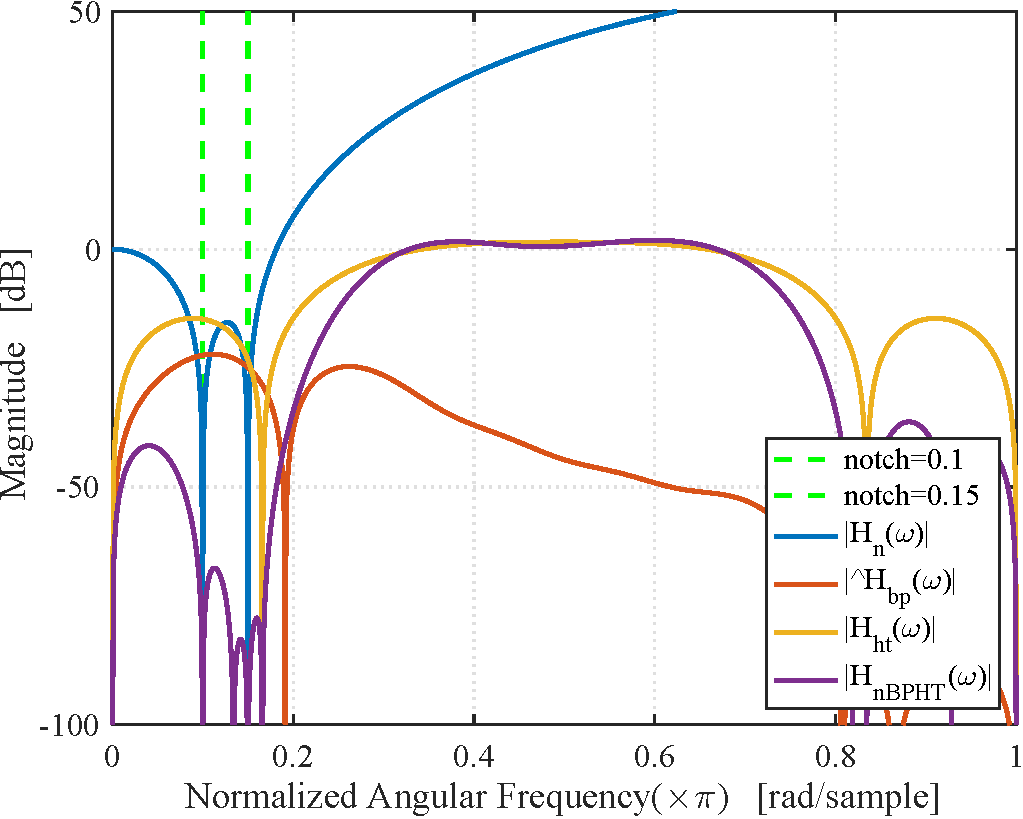
\includegraphics[width=8cm]
    		{Figure/figure01.pdf}
    \caption{のっちだおおおおおおお}
    \label{fig:man}
\end{figure}     <--第4章 まとめ
%#!platex main.tex
\chapter*{謝辞}
\addcontentsline{toc}{chapter}{謝辞} 
Other/thanks.texで文章を編集して下さい
%本研究にあたり,多大なるご指導とご助
%言を賜わりました.伊丹~ 誠教授,大野~光平先生に深く感謝いたします.また,色々
%な面でご協力いただいた伊丹研究室の大学院生の皆様,卒業研究生に対しまして
%も,心より感謝致します.最後に感謝の意を表して,本論文の謝辞とさせて頂きま
%す.

              <--謝辞
%#!platex main.tex
\chapter*{発表論文}
\addcontentsline{toc}{chapter}{発表論文}
\def\essection#1{\section*{#1}\addcontentsline{toc}{section}{#1}}

\essection{A.査読あり論文}
\begin{itemize}
\item Other/publicationで編集して下さい
\end{itemize}


\essection{B.国際会議}

\essection{C.研究会}

\essection{D.大会}

         <--発表論文リスト
\include{Other/bibliography}        <--参考文献
\end{verbatim}
です.
\begin{verbatim}
%#!platex main.tex
\chapter*{発表論文}
\addcontentsline{toc}{chapter}{発表論文}
\def\essection#1{\section*{#1}\addcontentsline{toc}{section}{#1}}

\essection{A.査読あり論文}
\begin{itemize}
\item Other/publicationで編集して下さい
\end{itemize}


\essection{B.国際会議}

\essection{C.研究会}

\essection{D.大会}


\end{verbatim}
は発表論文リストファイルですので卒論の場合,\verb|%|でコメントアウトして
 おいてください.

コンパイルの方法は

\framebox{\tt jlatex main.tex}

です.
しかし,これだけだと,目次が構成できないので,もう一度

\framebox{\tt jlatex main.tex}

とやると,目次も構成されます.
ちなみに,

\framebox{\tt make;make final}

とすると,main.psまではきます.
最後の最後の提出の時まではあまり使わないと思います.
修論などで,100ページ以上になると,psファイルがかなりでかくなるので,
 quotaに気をつけてください.
あと

\framebox{\tt make clean}

とすると,ディレクトリ内の掃除ができるのたまにやってもいいかも知れません.

また,yatexを利用すると,圧倒的に効率が良くなります.
この時,各LaTeXファイルに
\begin{verbatim}
%#!jlatex main.tex	
\end{verbatim}
という一行を加えておくと,どのLaTeXファイルからでもmain.texが呼べるので,
現在作業中のLaTeXファイル上で,jlatex main.texができます.
これはかなり便利です.
\section{おまけ}
図や表の引用で\verb|\ref|を利用すると思いますが,このスタイルでは
\verb|\ref{ラベル名}|とすると自動的に{\gt 図 {\bf 1}}のように出力するよ
うになっています.
これは表の引用,本文の引用においても同様です.
これが嫌な人はitlbthesis2012.styの最後の
\begin{verbatim}
\def\p@chapter{{\dg 本文}}
\def\p@section{{\dg 本文}}
\def\p@subsection{{\dg 本文}}
\def\p@subsubsection{{\dg 本文}}
\def\p@figure{{\dg 図}}
\def\p@table{{\dg 表}}
\let\origref=\ref
\def\ref#1{{\bf \origref{#1}}}
\end{verbatim}
を削除してください.


   <--第2章 スタイルファイルの使い方
\include{Figure/figure}             <--第3章 絵の貼り方
%#!platex main.tex
\chapter{序論}

\section{章タイトル}
参考文献のテスト\cite{樋口龍雄2000}.
"bibliography.bib"の中身をいじると変更できます.

あいうえおかきくけこ
正弦波の周波数推定はレーダーやソナー,通信,医療などの領域で幅広く研究されてきた課題である\cite{R.G.McKilliam,K.Wang,D.Rife}.
一般に,単一正弦波に対する周波数推定を行う場合,アナログ信号であれば周波数カウンタを用いる手法,ディジタル信号の場合,相関を用いた手法やヒルベルト変換器を用いる手法が提案されている.
周波数カウンタを用いた手法では,1周期に対して基準クロックを用いて測定し,その逆数から周波数を求めるレシプロカル方式の周波数カウンタが知られている.しかしこの手法を用いる場合,周波数が変化すると出力間隔が不等間隔になる.そのため,計測値に対して,ディジタル処理を行う場合には補完処理などの工夫が必要となるため,サンプルごとに周波数の推定値が出力されるヒルベルト変換器を用いた手法が提案されている.\\
 ヒルベルト変換器を用いた手法では,入力を実部,出力を虚部とする複素信号の一種である解析信号の位相を時間微分し,瞬時角周波数から瞬時周波数を推定することができる.従来,ヒルベルト変換器は有限次数のFIRフィルタとして設計されるため振幅特性にリプルが生じ,出力は振動する場合がある.高尾ら\cite{高尾可変なし,高尾可変あり}は振動成分の周波数が入力周波数の偶数倍であることを理論的に示し,これを伝送零点を有する可変FIRフィルタを用いて振動成分を除去することで,低次数なヒルベルト変換器を用いても,単一正弦波の高精度な瞬時周波数推定が可能となることを示した.
%高尾さんのやつと関連させてノイズを取れることを書きたいなら,どういうノイズが取れて,どういうノイズがダメなのか明記する必要がある.
しかし実際にはノイズを含む信号を解析する必要がある.一般に,ノイズを含む信号に対して,ヒルベルト変換を行うためには,あらかじめ帯域通過フィルタによりノイズを低減させた後に,ヒルベルト変換器を縦続接続する方法が考えられる.しかし,帯域通過フィルタとヒルベルト変換器を1つのフィルタとして見た場合,全体の次数が増加し,結果として遅延や回路規模の増大につながり好ましくない.\\
 そこで本稿では,阻止域を有するヒルベルト変換器に対し,指定した位置に伝送零点を置くことで,ノイズを除去しながらヒルベルト変換可能なフィルタを設計する.阻止域を有するヒルベルト変換器を設計する場合,本来であれば阻止域において十分な減衰量を確保するために多くのフィルタ次数が必要となる.しかし,特定の周波数成分にノイズが含まれることがわかっている場合,その周波数成分のみに伝送零点を入れることにより,特定のノイズのみ除去しながらヒルベルト変換を行うことができ,減衰量を確保するために必要な次数を削減することができる.
最後に設計例を示し,提案法の有効性を確認する.
\section{指定した位置に伝送零点を有するヒルベルト変換器}
本章では提案するフィルタの設計問題について記す.提案するフィルタは,阻止域の指定した位置に伝送零点を有するヒルベルト変換器である.本稿で設計するフィルタの振幅理想特性を図\ref{ideal_resp}に示す.またフィルタの振幅理想特性は正規化角周波数$\omega$を用いて,

\begin{figure}[tb]
    \centering
    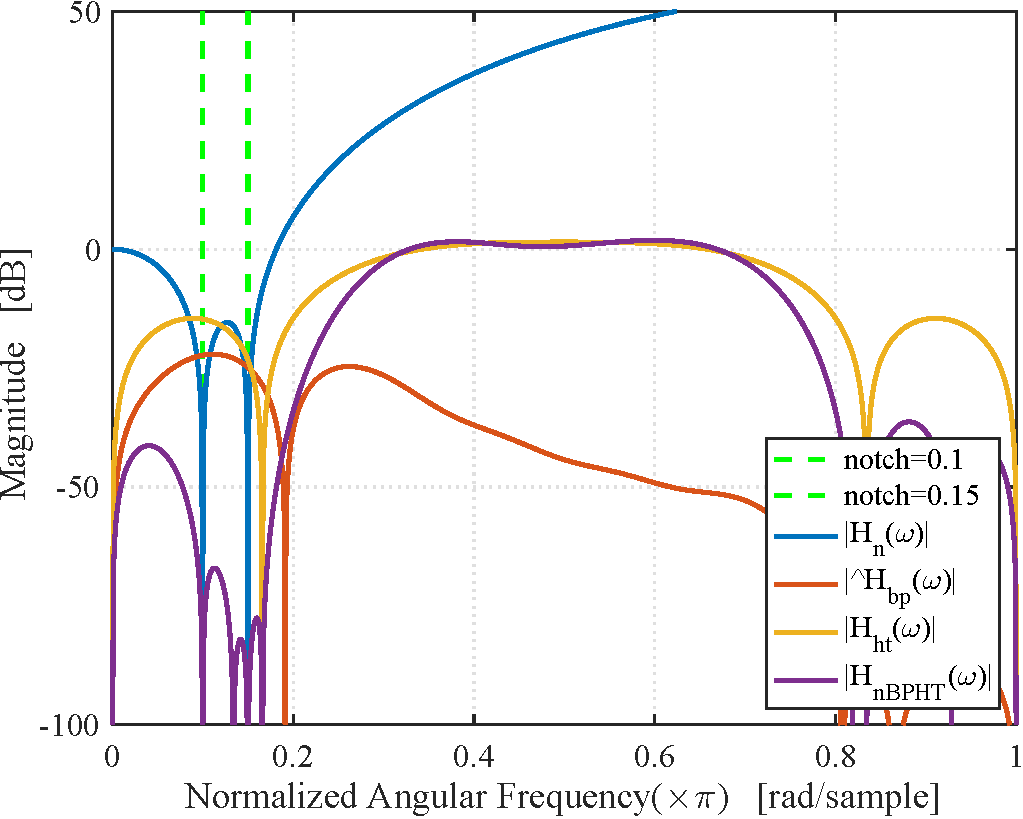
\includegraphics[width=8cm]
    		{Figure/figure01.pdf}
    \caption{のっちだおおおおおおお}
    \label{fig:man}
\end{figure}     <--第4章 まとめ
%#!platex main.tex
\chapter*{謝辞}
\addcontentsline{toc}{chapter}{謝辞} 
Other/thanks.texで文章を編集して下さい
%本研究にあたり,多大なるご指導とご助
%言を賜わりました.伊丹~ 誠教授,大野~光平先生に深く感謝いたします.また,色々
%な面でご協力いただいた伊丹研究室の大学院生の皆様,卒業研究生に対しまして
%も,心より感謝致します.最後に感謝の意を表して,本論文の謝辞とさせて頂きま
%す.

              <--謝辞
%#!platex main.tex
\chapter*{発表論文}
\addcontentsline{toc}{chapter}{発表論文}
\def\essection#1{\section*{#1}\addcontentsline{toc}{section}{#1}}

\essection{A.査読あり論文}
\begin{itemize}
\item Other/publicationで編集して下さい
\end{itemize}


\essection{B.国際会議}

\essection{C.研究会}

\essection{D.大会}

         <--発表論文リスト
\include{Other/bibliography}        <--参考文献
\end{verbatim}
です.
\begin{verbatim}
%#!platex main.tex
\chapter*{発表論文}
\addcontentsline{toc}{chapter}{発表論文}
\def\essection#1{\section*{#1}\addcontentsline{toc}{section}{#1}}

\essection{A.査読あり論文}
\begin{itemize}
\item Other/publicationで編集して下さい
\end{itemize}


\essection{B.国際会議}

\essection{C.研究会}

\essection{D.大会}


\end{verbatim}
は発表論文リストファイルですので卒論の場合,\verb|%|でコメントアウトして
 おいてください.

コンパイルの方法は

\framebox{\tt jlatex main.tex}

です.
しかし,これだけだと,目次が構成できないので,もう一度

\framebox{\tt jlatex main.tex}

とやると,目次も構成されます.
ちなみに,

\framebox{\tt make;make final}

とすると,main.psまではきます.
最後の最後の提出の時まではあまり使わないと思います.
修論などで,100ページ以上になると,psファイルがかなりでかくなるので,
 quotaに気をつけてください.
あと

\framebox{\tt make clean}

とすると,ディレクトリ内の掃除ができるのたまにやってもいいかも知れません.

また,yatexを利用すると,圧倒的に効率が良くなります.
この時,各LaTeXファイルに
\begin{verbatim}
%#!jlatex main.tex	
\end{verbatim}
という一行を加えておくと,どのLaTeXファイルからでもmain.texが呼べるので,
現在作業中のLaTeXファイル上で,jlatex main.texができます.
これはかなり便利です.
\section{おまけ}
図や表の引用で\verb|\ref|を利用すると思いますが,このスタイルでは
\verb|\ref{ラベル名}|とすると自動的に{\gt 図 {\bf 1}}のように出力するよ
うになっています.
これは表の引用,本文の引用においても同様です.
これが嫌な人はitlbthesis2012.styの最後の
\begin{verbatim}
\def\p@chapter{{\dg 本文}}
\def\p@section{{\dg 本文}}
\def\p@subsection{{\dg 本文}}
\def\p@subsubsection{{\dg 本文}}
\def\p@figure{{\dg 図}}
\def\p@table{{\dg 表}}
\let\origref=\ref
\def\ref#1{{\bf \origref{#1}}}
\end{verbatim}
を削除してください.



\include{Figure/figure}
%#!platex main.tex
\chapter{序論}

\section{章タイトル}
参考文献のテスト\cite{樋口龍雄2000}.
"bibliography.bib"の中身をいじると変更できます.

あいうえおかきくけこ
正弦波の周波数推定はレーダーやソナー,通信,医療などの領域で幅広く研究されてきた課題である\cite{R.G.McKilliam,K.Wang,D.Rife}.
一般に,単一正弦波に対する周波数推定を行う場合,アナログ信号であれば周波数カウンタを用いる手法,ディジタル信号の場合,相関を用いた手法やヒルベルト変換器を用いる手法が提案されている.
周波数カウンタを用いた手法では,1周期に対して基準クロックを用いて測定し,その逆数から周波数を求めるレシプロカル方式の周波数カウンタが知られている.しかしこの手法を用いる場合,周波数が変化すると出力間隔が不等間隔になる.そのため,計測値に対して,ディジタル処理を行う場合には補完処理などの工夫が必要となるため,サンプルごとに周波数の推定値が出力されるヒルベルト変換器を用いた手法が提案されている.\\
 ヒルベルト変換器を用いた手法では,入力を実部,出力を虚部とする複素信号の一種である解析信号の位相を時間微分し,瞬時角周波数から瞬時周波数を推定することができる.従来,ヒルベルト変換器は有限次数のFIRフィルタとして設計されるため振幅特性にリプルが生じ,出力は振動する場合がある.高尾ら\cite{高尾可変なし,高尾可変あり}は振動成分の周波数が入力周波数の偶数倍であることを理論的に示し,これを伝送零点を有する可変FIRフィルタを用いて振動成分を除去することで,低次数なヒルベルト変換器を用いても,単一正弦波の高精度な瞬時周波数推定が可能となることを示した.
%高尾さんのやつと関連させてノイズを取れることを書きたいなら,どういうノイズが取れて,どういうノイズがダメなのか明記する必要がある.
しかし実際にはノイズを含む信号を解析する必要がある.一般に,ノイズを含む信号に対して,ヒルベルト変換を行うためには,あらかじめ帯域通過フィルタによりノイズを低減させた後に,ヒルベルト変換器を縦続接続する方法が考えられる.しかし,帯域通過フィルタとヒルベルト変換器を1つのフィルタとして見た場合,全体の次数が増加し,結果として遅延や回路規模の増大につながり好ましくない.\\
 そこで本稿では,阻止域を有するヒルベルト変換器に対し,指定した位置に伝送零点を置くことで,ノイズを除去しながらヒルベルト変換可能なフィルタを設計する.阻止域を有するヒルベルト変換器を設計する場合,本来であれば阻止域において十分な減衰量を確保するために多くのフィルタ次数が必要となる.しかし,特定の周波数成分にノイズが含まれることがわかっている場合,その周波数成分のみに伝送零点を入れることにより,特定のノイズのみ除去しながらヒルベルト変換を行うことができ,減衰量を確保するために必要な次数を削減することができる.
最後に設計例を示し,提案法の有効性を確認する.
\section{指定した位置に伝送零点を有するヒルベルト変換器}
本章では提案するフィルタの設計問題について記す.提案するフィルタは,阻止域の指定した位置に伝送零点を有するヒルベルト変換器である.本稿で設計するフィルタの振幅理想特性を図\ref{ideal_resp}に示す.またフィルタの振幅理想特性は正規化角周波数$\omega$を用いて,

\begin{figure}[tb]
    \centering
    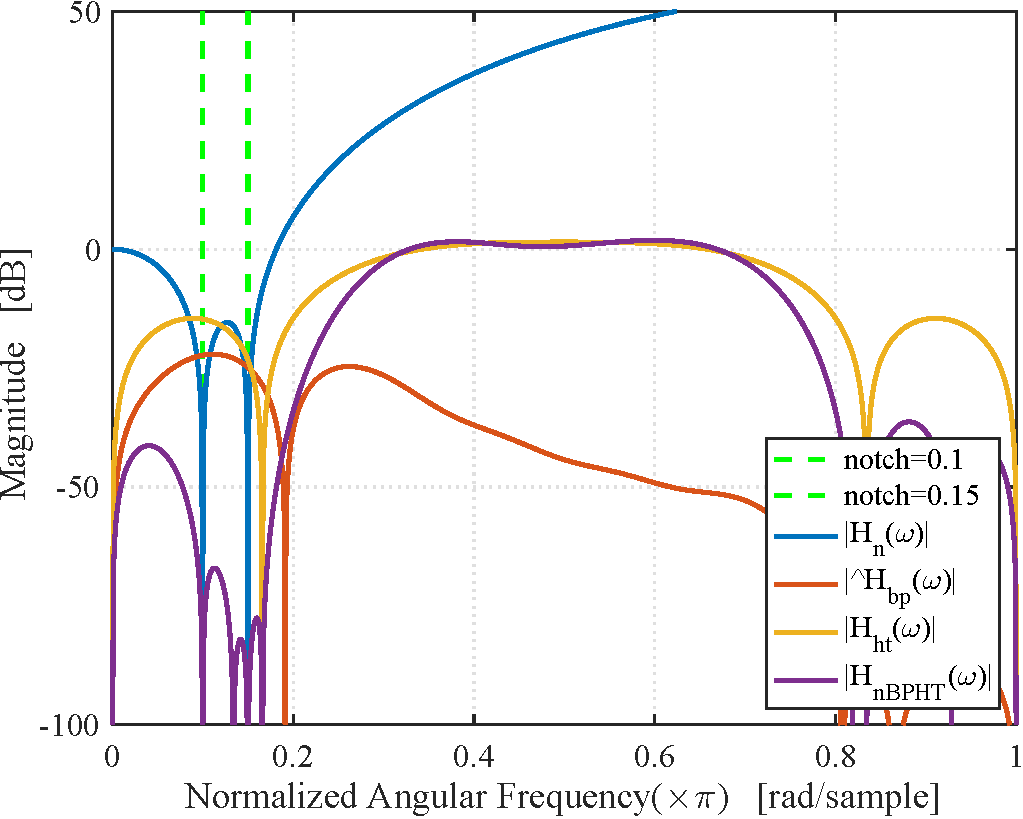
\includegraphics[width=8cm]
    		{Figure/figure01.pdf}
    \caption{のっちだおおおおおおお}
    \label{fig:man}
\end{figure}
%#!platex main.tex
\chapter*{謝辞}
\addcontentsline{toc}{chapter}{謝辞} 
Other/thanks.texで文章を編集して下さい
%本研究にあたり,多大なるご指導とご助
%言を賜わりました.伊丹~ 誠教授,大野~光平先生に深く感謝いたします.また,色々
%な面でご協力いただいた伊丹研究室の大学院生の皆様,卒業研究生に対しまして
%も,心より感謝致します.最後に感謝の意を表して,本論文の謝辞とさせて頂きま
%す.


\include{Other/bibliography}
%#!platex main.tex
\chapter*{発表論文}
\addcontentsline{toc}{chapter}{発表論文}
\def\essection#1{\section*{#1}\addcontentsline{toc}{section}{#1}}

\essection{A.査読あり論文}
\begin{itemize}
\item Other/publicationで編集して下さい
\end{itemize}


\essection{B.国際会議}

\essection{C.研究会}

\essection{D.大会}


\end{document}
\end{verbatim}
のようになっています.

\begin{verbatim}
\documentstyle[12pt,eclepsf,itlbthesis2000,eclclass]{j-report}
\end{verbatim}
でeclclassは\ref{itlbthesis2000ディレクトリ構成}を書くために必要なだけ
です.
ちなみにeclclass.styは\ref{itlbthesis2000ディレクトリ構成}のようなディ
レクトリ構造を書くのに便利なスタイルですが,使わなければ,
\begin{verbatim}
\documentstyle[12pt,eclepsf,itlbthesis2000]{j-report}
\end{verbatim}
としておいて結構です.
12pt.styは文字の大きさを指定するものではずさないでください.
またecleps.styはepsファイルを取り込むものなので,epsファイルを一枚も使わ
ない人ははずしても結構です(たぶんそんなことはない).
更に,スタイルファイル(例えばhere.sty)を追加する場合,
\begin{verbatim}
\documentstyle[12pt,eclepsf,itlbthesis2000,here]{j-report}
\end{verbatim}
のようにすればOKです.

\begin{verbatim}
\begin{document}
\itlbtitle    <---表紙を作ってます
\makeabstract <---アブストラクトを作ってます
\makecontents <---目次を作ってます
\end{verbatim}
は変更しないでください.

\begin{verbatim}
\include{}	
\end{verbatim}
は異なるLaTeXソースをincludeするもので,各章毎に別々のディレクトリで文章を
作ってください.

このようにする理由は次章で述べられているので,次の章は必ず読んでください.

従って,main.texで書き換える必要があるのは
\begin{verbatim}
\include{Introduction/introduction} <--第1章 序論
%#!platex main.tex

\chapter{このスタイルの使い方}
\section{このスタイルファイルについて}
このスタイルファイルの原型は1998年に修士を修了した下村さんが作成したもの
です.
それに初期設定ファイル等を加えて,LaTeXのマクロをブラックボックス化し,
あまりLaTeXのスタイルをわからない人でも使いやすいようにしたつもりです.
本来の目的は,PDF化に際しての編集者の負荷軽減の目的ですが,それほど難し
いスタイルではないので,解析して自分用に書き換えてもらっても結構です.
また,YaTeXを利用する事を前提にして作っている部分もあるので,なじみにく
い人は,過去のスタイルを利用するか,YaTeXを覚えてください.\\
\\
2012.11.20\\
itlbthesis2000.sty(j-tex用)をplatex用に改良したitlbthesis2012.styを作成しました.\\
以下の文章はitlbthesis2000の時のものとなっているので,注意して下さい.
また,バックアップを/home/yakou/Public/Styleの中に保存しておくので,何かありましたら参照してください.
\\
\section{ファイル構成}
まず,

\framebox{\tt gzip -d itlbthesis2000.tar.gz}

とし,

\framebox{\tt tar xvf itlbthesis2000.tar}

とすると,itlbthesis2000というディレクトリができると思います.

\framebox{\tt cd itlbthesis2000}

で中に入ると,その中身は\ref{itlbthesis2000ディレクトリ構成}のようになっ
ています.

ここで,とりあえず,

\framebox{\tt jlatex main.tex}

\framebox{\tt jlatex main.tex}

と2回jlatexをmain.texに対してかけてください.
そこにmain.dviがあるので,

\framebox{\tt xdvi-gs main.dvi}

とすると,このDVIファイルを見ることができます.
\section{設定の方法}
\begin{figure}[htb]
 \begin{center}
  \begin{classify}{\fbox{itlbthesis2000}\hspace*{5cm} $\circ$は全員必須,
   $*$は修士論文のみ必須}
   \class{
   \begin{classify}{\fbox{Introduction}(第1章)}
    \class{introduction.tex(第1章の\LaTeX ソース)}
   \end{classify}
   }
   \class{
   \begin{classify}{\fbox{StyleManual}第2章)}
    \class{stylemanual.tex(第2章の\LaTeX ソース)}
   \end{classify}
   }
   \class{
   \begin{classify}{\fbox{Figure}(第3章)}
    \class{
    \begin{classify}{\fbox{EPS}(第3章用EPSディレクトリ)}
     \class{hogehoge.eps(第3章に関するeps)}
    \end{classify}
    }
    \class{
    \begin{classify}{\fbox{XVD}(第3章用XVDディレクトリ)}
     \class{hogehoge.xvd(第3章に関するxvd)}
    \end{classify}
    }
    \class{figure.tex(第3章の\LaTeX ソース)}
   \end{classify}
   }
   \class{
   \begin{classify}{\fbox{Conclusion}(第4章)}
    \class{conclusion.tex(第4章に関する\LaTeX ソース)}
   \end{classify}
   }
   \class{
   \begin{classify}{\fbox{Other}(その他)}
    \class{abstract.tex(和文アブストラクト$)^{\circ}$}
    \class{abstract\_e.tex(英文アブストラクト$)^{*}$}
    \class{bibliography.tex(参考文献$)^{\circ}$}
    \class{publication.tex(発表論文$)^{*}$}
    \class{thanks.tex(謝辞$)^{\circ}$}
  \end{classify}
   }
   \class{Makefile(メイクファイル$)^{\circ}$}
   \class{eclclass.sty(この絵を書くためのだけのスタイル)}
   \class{init\_thesis.sty(初期設定ファイル$)^{\circ}$}
   \class{itlbthesis2000.sty(メインスタイルファイル$)^{\circ}$}
   \class{main.tex(メイン\LaTeX ソース$)^{\circ}$}
   \class{refcheck.sty(参照チェックスタイル)}
  \end{classify}
 \end{center}
 \caption{itlbthesis2000ディレクトリ構成}
 \label{itlbthesis2000ディレクトリ構成}
\end{figure}
\ref{itlbthesis2000ディレクトリ構成}を見てください.
この中で,itlbthesis2000.styはいじらなくても良いです.
\subsection{init\_thesis.styの書き方}
init\_thesis.styファイルは,初期設定ファイルです.中身は
\begin{verbatim}
%卒業論文の場合   \bm{卒業}
%修士論文の場合   \bm{修士}
\bm{修士}
%伊藤研究室の場合   \lab{伊藤}
%伊丹研究室の場合   \lab{伊丹}
\lab{伊藤}
%西暦の年   \year{}
\year{2001}
%平成の年   \heisei{}
\heisei{12}
%提出する月 \month{}
\month{2}
%論文の和文メインタイトル   \title{}
\title{卒業論文,修士論文の書き方}
%論文の英文メインタイトル(修論のみ)   \titleE{}
%卒論は空欄でOK
\titleE{How to draw up a bachelor's and master's thesis for our laboratory}
%論文の和文サブタイトル   \subtitle{}
%特になければ空欄でもOK 
\subtitle{サブタイトル}
%論文の英文サブタイトル(修論のみ)   \subtitleE{}
%特になければ空欄でもOK
%卒論は空欄でOK
\subtitleE{English sub-title}
%自分の学籍番号   \num{}
\num{8100701}
%自分の日本語の名前   \author{}
\author{藤井 雅弘}
%自分の英語の名前(修論のみ)   \authorE{}
%卒論は空欄でOK
\authorE{Masahiro Fujii}
%和文アブストラクトファイルの指定   \abstract{}
\abstract{Other/abstract.tex}	
%英文アブストラクトファイルの指定(修論のみ)   \abstractE{}
%卒論は空欄でOK
\abstruatE{Other/abstract_e.tex}	
\end{verbatim}
となってきます.
自分で勝手に書き換えてください.

卒論生は''修論のみ''となっている所はそのままでも,空欄でも結構です.
但し,コメントアウトしたり,その行自体を削除したりするとえらいことになり
ます.
一番上の\verb|\bm|を\verb|\bm{卒業}|としておけば,修論のみとなっている所
は反映されません.
\subsection{main.texの書き方}
このmain.dviのTeXソースmain.texは
\begin{verbatim}
\documentstyle[12pt,eclepsf,itlbthesis2000,eclclass]{j-report}
\begin{document}
\itlbtitle
\makeabstract
\makecontents
\include{Introduction/introduction}
%#!platex main.tex

\chapter{このスタイルの使い方}
\section{このスタイルファイルについて}
このスタイルファイルの原型は1998年に修士を修了した下村さんが作成したもの
です.
それに初期設定ファイル等を加えて,LaTeXのマクロをブラックボックス化し,
あまりLaTeXのスタイルをわからない人でも使いやすいようにしたつもりです.
本来の目的は,PDF化に際しての編集者の負荷軽減の目的ですが,それほど難し
いスタイルではないので,解析して自分用に書き換えてもらっても結構です.
また,YaTeXを利用する事を前提にして作っている部分もあるので,なじみにく
い人は,過去のスタイルを利用するか,YaTeXを覚えてください.\\
\\
2012.11.20\\
itlbthesis2000.sty(j-tex用)をplatex用に改良したitlbthesis2012.styを作成しました.\\
以下の文章はitlbthesis2000の時のものとなっているので,注意して下さい.
また,バックアップを/home/yakou/Public/Styleの中に保存しておくので,何かありましたら参照してください.
\\
\section{ファイル構成}
まず,

\framebox{\tt gzip -d itlbthesis2000.tar.gz}

とし,

\framebox{\tt tar xvf itlbthesis2000.tar}

とすると,itlbthesis2000というディレクトリができると思います.

\framebox{\tt cd itlbthesis2000}

で中に入ると,その中身は\ref{itlbthesis2000ディレクトリ構成}のようになっ
ています.

ここで,とりあえず,

\framebox{\tt jlatex main.tex}

\framebox{\tt jlatex main.tex}

と2回jlatexをmain.texに対してかけてください.
そこにmain.dviがあるので,

\framebox{\tt xdvi-gs main.dvi}

とすると,このDVIファイルを見ることができます.
\section{設定の方法}
\begin{figure}[htb]
 \begin{center}
  \begin{classify}{\fbox{itlbthesis2000}\hspace*{5cm} $\circ$は全員必須,
   $*$は修士論文のみ必須}
   \class{
   \begin{classify}{\fbox{Introduction}(第1章)}
    \class{introduction.tex(第1章の\LaTeX ソース)}
   \end{classify}
   }
   \class{
   \begin{classify}{\fbox{StyleManual}第2章)}
    \class{stylemanual.tex(第2章の\LaTeX ソース)}
   \end{classify}
   }
   \class{
   \begin{classify}{\fbox{Figure}(第3章)}
    \class{
    \begin{classify}{\fbox{EPS}(第3章用EPSディレクトリ)}
     \class{hogehoge.eps(第3章に関するeps)}
    \end{classify}
    }
    \class{
    \begin{classify}{\fbox{XVD}(第3章用XVDディレクトリ)}
     \class{hogehoge.xvd(第3章に関するxvd)}
    \end{classify}
    }
    \class{figure.tex(第3章の\LaTeX ソース)}
   \end{classify}
   }
   \class{
   \begin{classify}{\fbox{Conclusion}(第4章)}
    \class{conclusion.tex(第4章に関する\LaTeX ソース)}
   \end{classify}
   }
   \class{
   \begin{classify}{\fbox{Other}(その他)}
    \class{abstract.tex(和文アブストラクト$)^{\circ}$}
    \class{abstract\_e.tex(英文アブストラクト$)^{*}$}
    \class{bibliography.tex(参考文献$)^{\circ}$}
    \class{publication.tex(発表論文$)^{*}$}
    \class{thanks.tex(謝辞$)^{\circ}$}
  \end{classify}
   }
   \class{Makefile(メイクファイル$)^{\circ}$}
   \class{eclclass.sty(この絵を書くためのだけのスタイル)}
   \class{init\_thesis.sty(初期設定ファイル$)^{\circ}$}
   \class{itlbthesis2000.sty(メインスタイルファイル$)^{\circ}$}
   \class{main.tex(メイン\LaTeX ソース$)^{\circ}$}
   \class{refcheck.sty(参照チェックスタイル)}
  \end{classify}
 \end{center}
 \caption{itlbthesis2000ディレクトリ構成}
 \label{itlbthesis2000ディレクトリ構成}
\end{figure}
\ref{itlbthesis2000ディレクトリ構成}を見てください.
この中で,itlbthesis2000.styはいじらなくても良いです.
\subsection{init\_thesis.styの書き方}
init\_thesis.styファイルは,初期設定ファイルです.中身は
\begin{verbatim}
%卒業論文の場合   \bm{卒業}
%修士論文の場合   \bm{修士}
\bm{修士}
%伊藤研究室の場合   \lab{伊藤}
%伊丹研究室の場合   \lab{伊丹}
\lab{伊藤}
%西暦の年   \year{}
\year{2001}
%平成の年   \heisei{}
\heisei{12}
%提出する月 \month{}
\month{2}
%論文の和文メインタイトル   \title{}
\title{卒業論文,修士論文の書き方}
%論文の英文メインタイトル(修論のみ)   \titleE{}
%卒論は空欄でOK
\titleE{How to draw up a bachelor's and master's thesis for our laboratory}
%論文の和文サブタイトル   \subtitle{}
%特になければ空欄でもOK 
\subtitle{サブタイトル}
%論文の英文サブタイトル(修論のみ)   \subtitleE{}
%特になければ空欄でもOK
%卒論は空欄でOK
\subtitleE{English sub-title}
%自分の学籍番号   \num{}
\num{8100701}
%自分の日本語の名前   \author{}
\author{藤井 雅弘}
%自分の英語の名前(修論のみ)   \authorE{}
%卒論は空欄でOK
\authorE{Masahiro Fujii}
%和文アブストラクトファイルの指定   \abstract{}
\abstract{Other/abstract.tex}	
%英文アブストラクトファイルの指定(修論のみ)   \abstractE{}
%卒論は空欄でOK
\abstruatE{Other/abstract_e.tex}	
\end{verbatim}
となってきます.
自分で勝手に書き換えてください.

卒論生は''修論のみ''となっている所はそのままでも,空欄でも結構です.
但し,コメントアウトしたり,その行自体を削除したりするとえらいことになり
ます.
一番上の\verb|\bm|を\verb|\bm{卒業}|としておけば,修論のみとなっている所
は反映されません.
\subsection{main.texの書き方}
このmain.dviのTeXソースmain.texは
\begin{verbatim}
\documentstyle[12pt,eclepsf,itlbthesis2000,eclclass]{j-report}
\begin{document}
\itlbtitle
\makeabstract
\makecontents
\include{Introduction/introduction}
%#!platex main.tex

\chapter{このスタイルの使い方}
\section{このスタイルファイルについて}
このスタイルファイルの原型は1998年に修士を修了した下村さんが作成したもの
です.
それに初期設定ファイル等を加えて,LaTeXのマクロをブラックボックス化し,
あまりLaTeXのスタイルをわからない人でも使いやすいようにしたつもりです.
本来の目的は,PDF化に際しての編集者の負荷軽減の目的ですが,それほど難し
いスタイルではないので,解析して自分用に書き換えてもらっても結構です.
また,YaTeXを利用する事を前提にして作っている部分もあるので,なじみにく
い人は,過去のスタイルを利用するか,YaTeXを覚えてください.\\
\\
2012.11.20\\
itlbthesis2000.sty(j-tex用)をplatex用に改良したitlbthesis2012.styを作成しました.\\
以下の文章はitlbthesis2000の時のものとなっているので,注意して下さい.
また,バックアップを/home/yakou/Public/Styleの中に保存しておくので,何かありましたら参照してください.
\\
\section{ファイル構成}
まず,

\framebox{\tt gzip -d itlbthesis2000.tar.gz}

とし,

\framebox{\tt tar xvf itlbthesis2000.tar}

とすると,itlbthesis2000というディレクトリができると思います.

\framebox{\tt cd itlbthesis2000}

で中に入ると,その中身は\ref{itlbthesis2000ディレクトリ構成}のようになっ
ています.

ここで,とりあえず,

\framebox{\tt jlatex main.tex}

\framebox{\tt jlatex main.tex}

と2回jlatexをmain.texに対してかけてください.
そこにmain.dviがあるので,

\framebox{\tt xdvi-gs main.dvi}

とすると,このDVIファイルを見ることができます.
\section{設定の方法}
\begin{figure}[htb]
 \begin{center}
  \begin{classify}{\fbox{itlbthesis2000}\hspace*{5cm} $\circ$は全員必須,
   $*$は修士論文のみ必須}
   \class{
   \begin{classify}{\fbox{Introduction}(第1章)}
    \class{introduction.tex(第1章の\LaTeX ソース)}
   \end{classify}
   }
   \class{
   \begin{classify}{\fbox{StyleManual}第2章)}
    \class{stylemanual.tex(第2章の\LaTeX ソース)}
   \end{classify}
   }
   \class{
   \begin{classify}{\fbox{Figure}(第3章)}
    \class{
    \begin{classify}{\fbox{EPS}(第3章用EPSディレクトリ)}
     \class{hogehoge.eps(第3章に関するeps)}
    \end{classify}
    }
    \class{
    \begin{classify}{\fbox{XVD}(第3章用XVDディレクトリ)}
     \class{hogehoge.xvd(第3章に関するxvd)}
    \end{classify}
    }
    \class{figure.tex(第3章の\LaTeX ソース)}
   \end{classify}
   }
   \class{
   \begin{classify}{\fbox{Conclusion}(第4章)}
    \class{conclusion.tex(第4章に関する\LaTeX ソース)}
   \end{classify}
   }
   \class{
   \begin{classify}{\fbox{Other}(その他)}
    \class{abstract.tex(和文アブストラクト$)^{\circ}$}
    \class{abstract\_e.tex(英文アブストラクト$)^{*}$}
    \class{bibliography.tex(参考文献$)^{\circ}$}
    \class{publication.tex(発表論文$)^{*}$}
    \class{thanks.tex(謝辞$)^{\circ}$}
  \end{classify}
   }
   \class{Makefile(メイクファイル$)^{\circ}$}
   \class{eclclass.sty(この絵を書くためのだけのスタイル)}
   \class{init\_thesis.sty(初期設定ファイル$)^{\circ}$}
   \class{itlbthesis2000.sty(メインスタイルファイル$)^{\circ}$}
   \class{main.tex(メイン\LaTeX ソース$)^{\circ}$}
   \class{refcheck.sty(参照チェックスタイル)}
  \end{classify}
 \end{center}
 \caption{itlbthesis2000ディレクトリ構成}
 \label{itlbthesis2000ディレクトリ構成}
\end{figure}
\ref{itlbthesis2000ディレクトリ構成}を見てください.
この中で,itlbthesis2000.styはいじらなくても良いです.
\subsection{init\_thesis.styの書き方}
init\_thesis.styファイルは,初期設定ファイルです.中身は
\begin{verbatim}
%卒業論文の場合   \bm{卒業}
%修士論文の場合   \bm{修士}
\bm{修士}
%伊藤研究室の場合   \lab{伊藤}
%伊丹研究室の場合   \lab{伊丹}
\lab{伊藤}
%西暦の年   \year{}
\year{2001}
%平成の年   \heisei{}
\heisei{12}
%提出する月 \month{}
\month{2}
%論文の和文メインタイトル   \title{}
\title{卒業論文,修士論文の書き方}
%論文の英文メインタイトル(修論のみ)   \titleE{}
%卒論は空欄でOK
\titleE{How to draw up a bachelor's and master's thesis for our laboratory}
%論文の和文サブタイトル   \subtitle{}
%特になければ空欄でもOK 
\subtitle{サブタイトル}
%論文の英文サブタイトル(修論のみ)   \subtitleE{}
%特になければ空欄でもOK
%卒論は空欄でOK
\subtitleE{English sub-title}
%自分の学籍番号   \num{}
\num{8100701}
%自分の日本語の名前   \author{}
\author{藤井 雅弘}
%自分の英語の名前(修論のみ)   \authorE{}
%卒論は空欄でOK
\authorE{Masahiro Fujii}
%和文アブストラクトファイルの指定   \abstract{}
\abstract{Other/abstract.tex}	
%英文アブストラクトファイルの指定(修論のみ)   \abstractE{}
%卒論は空欄でOK
\abstruatE{Other/abstract_e.tex}	
\end{verbatim}
となってきます.
自分で勝手に書き換えてください.

卒論生は''修論のみ''となっている所はそのままでも,空欄でも結構です.
但し,コメントアウトしたり,その行自体を削除したりするとえらいことになり
ます.
一番上の\verb|\bm|を\verb|\bm{卒業}|としておけば,修論のみとなっている所
は反映されません.
\subsection{main.texの書き方}
このmain.dviのTeXソースmain.texは
\begin{verbatim}
\documentstyle[12pt,eclepsf,itlbthesis2000,eclclass]{j-report}
\begin{document}
\itlbtitle
\makeabstract
\makecontents
\include{Introduction/introduction}
\include{StyleManual/stylemanual}
\include{Figure/figure}
\include{Conclusion/conclusion}
\include{Other/thanks}
\include{Other/bibliography}
\include{Other/publication}
\end{document}
\end{verbatim}
のようになっています.

\begin{verbatim}
\documentstyle[12pt,eclepsf,itlbthesis2000,eclclass]{j-report}
\end{verbatim}
でeclclassは\ref{itlbthesis2000ディレクトリ構成}を書くために必要なだけ
です.
ちなみにeclclass.styは\ref{itlbthesis2000ディレクトリ構成}のようなディ
レクトリ構造を書くのに便利なスタイルですが,使わなければ,
\begin{verbatim}
\documentstyle[12pt,eclepsf,itlbthesis2000]{j-report}
\end{verbatim}
としておいて結構です.
12pt.styは文字の大きさを指定するものではずさないでください.
またecleps.styはepsファイルを取り込むものなので,epsファイルを一枚も使わ
ない人ははずしても結構です(たぶんそんなことはない).
更に,スタイルファイル(例えばhere.sty)を追加する場合,
\begin{verbatim}
\documentstyle[12pt,eclepsf,itlbthesis2000,here]{j-report}
\end{verbatim}
のようにすればOKです.

\begin{verbatim}
\begin{document}
\itlbtitle    <---表紙を作ってます
\makeabstract <---アブストラクトを作ってます
\makecontents <---目次を作ってます
\end{verbatim}
は変更しないでください.

\begin{verbatim}
\include{}	
\end{verbatim}
は異なるLaTeXソースをincludeするもので,各章毎に別々のディレクトリで文章を
作ってください.

このようにする理由は次章で述べられているので,次の章は必ず読んでください.

従って,main.texで書き換える必要があるのは
\begin{verbatim}
\include{Introduction/introduction} <--第1章 序論
\include{StyleManual/stylemanual}   <--第2章 スタイルファイルの使い方
\include{Figure/figure}             <--第3章 絵の貼り方
\include{Conclusion/conclusion}     <--第4章 まとめ
\include{Other/thanks}              <--謝辞
\include{Other/publication}         <--発表論文リスト
\include{Other/bibliography}        <--参考文献
\end{verbatim}
です.
\begin{verbatim}
\include{Other/publication}
\end{verbatim}
は発表論文リストファイルですので卒論の場合,\verb|%|でコメントアウトして
 おいてください.

コンパイルの方法は

\framebox{\tt jlatex main.tex}

です.
しかし,これだけだと,目次が構成できないので,もう一度

\framebox{\tt jlatex main.tex}

とやると,目次も構成されます.
ちなみに,

\framebox{\tt make;make final}

とすると,main.psまではきます.
最後の最後の提出の時まではあまり使わないと思います.
修論などで,100ページ以上になると,psファイルがかなりでかくなるので,
 quotaに気をつけてください.
あと

\framebox{\tt make clean}

とすると,ディレクトリ内の掃除ができるのたまにやってもいいかも知れません.

また,yatexを利用すると,圧倒的に効率が良くなります.
この時,各LaTeXファイルに
\begin{verbatim}
%#!jlatex main.tex	
\end{verbatim}
という一行を加えておくと,どのLaTeXファイルからでもmain.texが呼べるので,
現在作業中のLaTeXファイル上で,jlatex main.texができます.
これはかなり便利です.
\section{おまけ}
図や表の引用で\verb|\ref|を利用すると思いますが,このスタイルでは
\verb|\ref{ラベル名}|とすると自動的に{\gt 図 {\bf 1}}のように出力するよ
うになっています.
これは表の引用,本文の引用においても同様です.
これが嫌な人はitlbthesis2012.styの最後の
\begin{verbatim}
\def\p@chapter{{\dg 本文}}
\def\p@section{{\dg 本文}}
\def\p@subsection{{\dg 本文}}
\def\p@subsubsection{{\dg 本文}}
\def\p@figure{{\dg 図}}
\def\p@table{{\dg 表}}
\let\origref=\ref
\def\ref#1{{\bf \origref{#1}}}
\end{verbatim}
を削除してください.



\include{Figure/figure}
%#!platex main.tex
\chapter{序論}

\section{章タイトル}
参考文献のテスト\cite{樋口龍雄2000}.
"bibliography.bib"の中身をいじると変更できます.

あいうえおかきくけこ
正弦波の周波数推定はレーダーやソナー,通信,医療などの領域で幅広く研究されてきた課題である\cite{R.G.McKilliam,K.Wang,D.Rife}.
一般に,単一正弦波に対する周波数推定を行う場合,アナログ信号であれば周波数カウンタを用いる手法,ディジタル信号の場合,相関を用いた手法やヒルベルト変換器を用いる手法が提案されている.
周波数カウンタを用いた手法では,1周期に対して基準クロックを用いて測定し,その逆数から周波数を求めるレシプロカル方式の周波数カウンタが知られている.しかしこの手法を用いる場合,周波数が変化すると出力間隔が不等間隔になる.そのため,計測値に対して,ディジタル処理を行う場合には補完処理などの工夫が必要となるため,サンプルごとに周波数の推定値が出力されるヒルベルト変換器を用いた手法が提案されている.\\
 ヒルベルト変換器を用いた手法では,入力を実部,出力を虚部とする複素信号の一種である解析信号の位相を時間微分し,瞬時角周波数から瞬時周波数を推定することができる.従来,ヒルベルト変換器は有限次数のFIRフィルタとして設計されるため振幅特性にリプルが生じ,出力は振動する場合がある.高尾ら\cite{高尾可変なし,高尾可変あり}は振動成分の周波数が入力周波数の偶数倍であることを理論的に示し,これを伝送零点を有する可変FIRフィルタを用いて振動成分を除去することで,低次数なヒルベルト変換器を用いても,単一正弦波の高精度な瞬時周波数推定が可能となることを示した.
%高尾さんのやつと関連させてノイズを取れることを書きたいなら,どういうノイズが取れて,どういうノイズがダメなのか明記する必要がある.
しかし実際にはノイズを含む信号を解析する必要がある.一般に,ノイズを含む信号に対して,ヒルベルト変換を行うためには,あらかじめ帯域通過フィルタによりノイズを低減させた後に,ヒルベルト変換器を縦続接続する方法が考えられる.しかし,帯域通過フィルタとヒルベルト変換器を1つのフィルタとして見た場合,全体の次数が増加し,結果として遅延や回路規模の増大につながり好ましくない.\\
 そこで本稿では,阻止域を有するヒルベルト変換器に対し,指定した位置に伝送零点を置くことで,ノイズを除去しながらヒルベルト変換可能なフィルタを設計する.阻止域を有するヒルベルト変換器を設計する場合,本来であれば阻止域において十分な減衰量を確保するために多くのフィルタ次数が必要となる.しかし,特定の周波数成分にノイズが含まれることがわかっている場合,その周波数成分のみに伝送零点を入れることにより,特定のノイズのみ除去しながらヒルベルト変換を行うことができ,減衰量を確保するために必要な次数を削減することができる.
最後に設計例を示し,提案法の有効性を確認する.
\section{指定した位置に伝送零点を有するヒルベルト変換器}
本章では提案するフィルタの設計問題について記す.提案するフィルタは,阻止域の指定した位置に伝送零点を有するヒルベルト変換器である.本稿で設計するフィルタの振幅理想特性を図\ref{ideal_resp}に示す.またフィルタの振幅理想特性は正規化角周波数$\omega$を用いて,

\begin{figure}[tb]
    \centering
    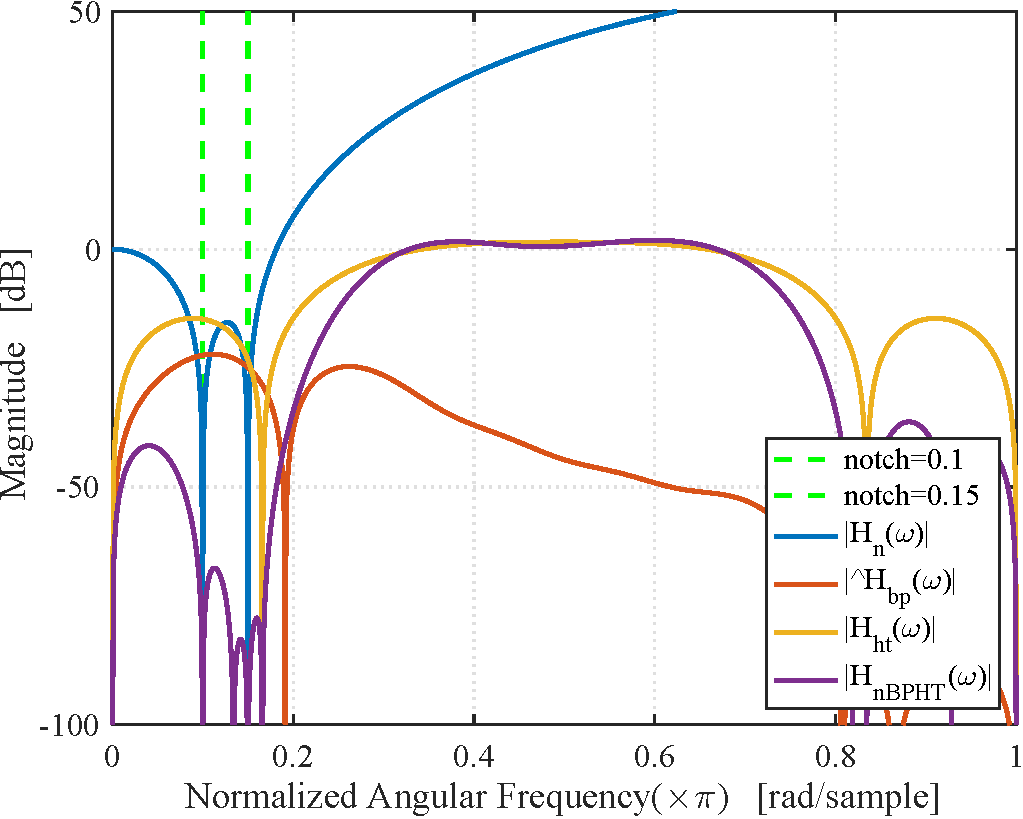
\includegraphics[width=8cm]
    		{Figure/figure01.pdf}
    \caption{のっちだおおおおおおお}
    \label{fig:man}
\end{figure}
%#!platex main.tex
\chapter*{謝辞}
\addcontentsline{toc}{chapter}{謝辞} 
Other/thanks.texで文章を編集して下さい
%本研究にあたり,多大なるご指導とご助
%言を賜わりました.伊丹~ 誠教授,大野~光平先生に深く感謝いたします.また,色々
%な面でご協力いただいた伊丹研究室の大学院生の皆様,卒業研究生に対しまして
%も,心より感謝致します.最後に感謝の意を表して,本論文の謝辞とさせて頂きま
%す.


\include{Other/bibliography}
%#!platex main.tex
\chapter*{発表論文}
\addcontentsline{toc}{chapter}{発表論文}
\def\essection#1{\section*{#1}\addcontentsline{toc}{section}{#1}}

\essection{A.査読あり論文}
\begin{itemize}
\item Other/publicationで編集して下さい
\end{itemize}


\essection{B.国際会議}

\essection{C.研究会}

\essection{D.大会}


\end{document}
\end{verbatim}
のようになっています.

\begin{verbatim}
\documentstyle[12pt,eclepsf,itlbthesis2000,eclclass]{j-report}
\end{verbatim}
でeclclassは\ref{itlbthesis2000ディレクトリ構成}を書くために必要なだけ
です.
ちなみにeclclass.styは\ref{itlbthesis2000ディレクトリ構成}のようなディ
レクトリ構造を書くのに便利なスタイルですが,使わなければ,
\begin{verbatim}
\documentstyle[12pt,eclepsf,itlbthesis2000]{j-report}
\end{verbatim}
としておいて結構です.
12pt.styは文字の大きさを指定するものではずさないでください.
またecleps.styはepsファイルを取り込むものなので,epsファイルを一枚も使わ
ない人ははずしても結構です(たぶんそんなことはない).
更に,スタイルファイル(例えばhere.sty)を追加する場合,
\begin{verbatim}
\documentstyle[12pt,eclepsf,itlbthesis2000,here]{j-report}
\end{verbatim}
のようにすればOKです.

\begin{verbatim}
\begin{document}
\itlbtitle    <---表紙を作ってます
\makeabstract <---アブストラクトを作ってます
\makecontents <---目次を作ってます
\end{verbatim}
は変更しないでください.

\begin{verbatim}
\include{}	
\end{verbatim}
は異なるLaTeXソースをincludeするもので,各章毎に別々のディレクトリで文章を
作ってください.

このようにする理由は次章で述べられているので,次の章は必ず読んでください.

従って,main.texで書き換える必要があるのは
\begin{verbatim}
\include{Introduction/introduction} <--第1章 序論
%#!platex main.tex

\chapter{このスタイルの使い方}
\section{このスタイルファイルについて}
このスタイルファイルの原型は1998年に修士を修了した下村さんが作成したもの
です.
それに初期設定ファイル等を加えて,LaTeXのマクロをブラックボックス化し,
あまりLaTeXのスタイルをわからない人でも使いやすいようにしたつもりです.
本来の目的は,PDF化に際しての編集者の負荷軽減の目的ですが,それほど難し
いスタイルではないので,解析して自分用に書き換えてもらっても結構です.
また,YaTeXを利用する事を前提にして作っている部分もあるので,なじみにく
い人は,過去のスタイルを利用するか,YaTeXを覚えてください.\\
\\
2012.11.20\\
itlbthesis2000.sty(j-tex用)をplatex用に改良したitlbthesis2012.styを作成しました.\\
以下の文章はitlbthesis2000の時のものとなっているので,注意して下さい.
また,バックアップを/home/yakou/Public/Styleの中に保存しておくので,何かありましたら参照してください.
\\
\section{ファイル構成}
まず,

\framebox{\tt gzip -d itlbthesis2000.tar.gz}

とし,

\framebox{\tt tar xvf itlbthesis2000.tar}

とすると,itlbthesis2000というディレクトリができると思います.

\framebox{\tt cd itlbthesis2000}

で中に入ると,その中身は\ref{itlbthesis2000ディレクトリ構成}のようになっ
ています.

ここで,とりあえず,

\framebox{\tt jlatex main.tex}

\framebox{\tt jlatex main.tex}

と2回jlatexをmain.texに対してかけてください.
そこにmain.dviがあるので,

\framebox{\tt xdvi-gs main.dvi}

とすると,このDVIファイルを見ることができます.
\section{設定の方法}
\begin{figure}[htb]
 \begin{center}
  \begin{classify}{\fbox{itlbthesis2000}\hspace*{5cm} $\circ$は全員必須,
   $*$は修士論文のみ必須}
   \class{
   \begin{classify}{\fbox{Introduction}(第1章)}
    \class{introduction.tex(第1章の\LaTeX ソース)}
   \end{classify}
   }
   \class{
   \begin{classify}{\fbox{StyleManual}第2章)}
    \class{stylemanual.tex(第2章の\LaTeX ソース)}
   \end{classify}
   }
   \class{
   \begin{classify}{\fbox{Figure}(第3章)}
    \class{
    \begin{classify}{\fbox{EPS}(第3章用EPSディレクトリ)}
     \class{hogehoge.eps(第3章に関するeps)}
    \end{classify}
    }
    \class{
    \begin{classify}{\fbox{XVD}(第3章用XVDディレクトリ)}
     \class{hogehoge.xvd(第3章に関するxvd)}
    \end{classify}
    }
    \class{figure.tex(第3章の\LaTeX ソース)}
   \end{classify}
   }
   \class{
   \begin{classify}{\fbox{Conclusion}(第4章)}
    \class{conclusion.tex(第4章に関する\LaTeX ソース)}
   \end{classify}
   }
   \class{
   \begin{classify}{\fbox{Other}(その他)}
    \class{abstract.tex(和文アブストラクト$)^{\circ}$}
    \class{abstract\_e.tex(英文アブストラクト$)^{*}$}
    \class{bibliography.tex(参考文献$)^{\circ}$}
    \class{publication.tex(発表論文$)^{*}$}
    \class{thanks.tex(謝辞$)^{\circ}$}
  \end{classify}
   }
   \class{Makefile(メイクファイル$)^{\circ}$}
   \class{eclclass.sty(この絵を書くためのだけのスタイル)}
   \class{init\_thesis.sty(初期設定ファイル$)^{\circ}$}
   \class{itlbthesis2000.sty(メインスタイルファイル$)^{\circ}$}
   \class{main.tex(メイン\LaTeX ソース$)^{\circ}$}
   \class{refcheck.sty(参照チェックスタイル)}
  \end{classify}
 \end{center}
 \caption{itlbthesis2000ディレクトリ構成}
 \label{itlbthesis2000ディレクトリ構成}
\end{figure}
\ref{itlbthesis2000ディレクトリ構成}を見てください.
この中で,itlbthesis2000.styはいじらなくても良いです.
\subsection{init\_thesis.styの書き方}
init\_thesis.styファイルは,初期設定ファイルです.中身は
\begin{verbatim}
%卒業論文の場合   \bm{卒業}
%修士論文の場合   \bm{修士}
\bm{修士}
%伊藤研究室の場合   \lab{伊藤}
%伊丹研究室の場合   \lab{伊丹}
\lab{伊藤}
%西暦の年   \year{}
\year{2001}
%平成の年   \heisei{}
\heisei{12}
%提出する月 \month{}
\month{2}
%論文の和文メインタイトル   \title{}
\title{卒業論文,修士論文の書き方}
%論文の英文メインタイトル(修論のみ)   \titleE{}
%卒論は空欄でOK
\titleE{How to draw up a bachelor's and master's thesis for our laboratory}
%論文の和文サブタイトル   \subtitle{}
%特になければ空欄でもOK 
\subtitle{サブタイトル}
%論文の英文サブタイトル(修論のみ)   \subtitleE{}
%特になければ空欄でもOK
%卒論は空欄でOK
\subtitleE{English sub-title}
%自分の学籍番号   \num{}
\num{8100701}
%自分の日本語の名前   \author{}
\author{藤井 雅弘}
%自分の英語の名前(修論のみ)   \authorE{}
%卒論は空欄でOK
\authorE{Masahiro Fujii}
%和文アブストラクトファイルの指定   \abstract{}
\abstract{Other/abstract.tex}	
%英文アブストラクトファイルの指定(修論のみ)   \abstractE{}
%卒論は空欄でOK
\abstruatE{Other/abstract_e.tex}	
\end{verbatim}
となってきます.
自分で勝手に書き換えてください.

卒論生は''修論のみ''となっている所はそのままでも,空欄でも結構です.
但し,コメントアウトしたり,その行自体を削除したりするとえらいことになり
ます.
一番上の\verb|\bm|を\verb|\bm{卒業}|としておけば,修論のみとなっている所
は反映されません.
\subsection{main.texの書き方}
このmain.dviのTeXソースmain.texは
\begin{verbatim}
\documentstyle[12pt,eclepsf,itlbthesis2000,eclclass]{j-report}
\begin{document}
\itlbtitle
\makeabstract
\makecontents
\include{Introduction/introduction}
\include{StyleManual/stylemanual}
\include{Figure/figure}
\include{Conclusion/conclusion}
\include{Other/thanks}
\include{Other/bibliography}
\include{Other/publication}
\end{document}
\end{verbatim}
のようになっています.

\begin{verbatim}
\documentstyle[12pt,eclepsf,itlbthesis2000,eclclass]{j-report}
\end{verbatim}
でeclclassは\ref{itlbthesis2000ディレクトリ構成}を書くために必要なだけ
です.
ちなみにeclclass.styは\ref{itlbthesis2000ディレクトリ構成}のようなディ
レクトリ構造を書くのに便利なスタイルですが,使わなければ,
\begin{verbatim}
\documentstyle[12pt,eclepsf,itlbthesis2000]{j-report}
\end{verbatim}
としておいて結構です.
12pt.styは文字の大きさを指定するものではずさないでください.
またecleps.styはepsファイルを取り込むものなので,epsファイルを一枚も使わ
ない人ははずしても結構です(たぶんそんなことはない).
更に,スタイルファイル(例えばhere.sty)を追加する場合,
\begin{verbatim}
\documentstyle[12pt,eclepsf,itlbthesis2000,here]{j-report}
\end{verbatim}
のようにすればOKです.

\begin{verbatim}
\begin{document}
\itlbtitle    <---表紙を作ってます
\makeabstract <---アブストラクトを作ってます
\makecontents <---目次を作ってます
\end{verbatim}
は変更しないでください.

\begin{verbatim}
\include{}	
\end{verbatim}
は異なるLaTeXソースをincludeするもので,各章毎に別々のディレクトリで文章を
作ってください.

このようにする理由は次章で述べられているので,次の章は必ず読んでください.

従って,main.texで書き換える必要があるのは
\begin{verbatim}
\include{Introduction/introduction} <--第1章 序論
\include{StyleManual/stylemanual}   <--第2章 スタイルファイルの使い方
\include{Figure/figure}             <--第3章 絵の貼り方
\include{Conclusion/conclusion}     <--第4章 まとめ
\include{Other/thanks}              <--謝辞
\include{Other/publication}         <--発表論文リスト
\include{Other/bibliography}        <--参考文献
\end{verbatim}
です.
\begin{verbatim}
\include{Other/publication}
\end{verbatim}
は発表論文リストファイルですので卒論の場合,\verb|%|でコメントアウトして
 おいてください.

コンパイルの方法は

\framebox{\tt jlatex main.tex}

です.
しかし,これだけだと,目次が構成できないので,もう一度

\framebox{\tt jlatex main.tex}

とやると,目次も構成されます.
ちなみに,

\framebox{\tt make;make final}

とすると,main.psまではきます.
最後の最後の提出の時まではあまり使わないと思います.
修論などで,100ページ以上になると,psファイルがかなりでかくなるので,
 quotaに気をつけてください.
あと

\framebox{\tt make clean}

とすると,ディレクトリ内の掃除ができるのたまにやってもいいかも知れません.

また,yatexを利用すると,圧倒的に効率が良くなります.
この時,各LaTeXファイルに
\begin{verbatim}
%#!jlatex main.tex	
\end{verbatim}
という一行を加えておくと,どのLaTeXファイルからでもmain.texが呼べるので,
現在作業中のLaTeXファイル上で,jlatex main.texができます.
これはかなり便利です.
\section{おまけ}
図や表の引用で\verb|\ref|を利用すると思いますが,このスタイルでは
\verb|\ref{ラベル名}|とすると自動的に{\gt 図 {\bf 1}}のように出力するよ
うになっています.
これは表の引用,本文の引用においても同様です.
これが嫌な人はitlbthesis2012.styの最後の
\begin{verbatim}
\def\p@chapter{{\dg 本文}}
\def\p@section{{\dg 本文}}
\def\p@subsection{{\dg 本文}}
\def\p@subsubsection{{\dg 本文}}
\def\p@figure{{\dg 図}}
\def\p@table{{\dg 表}}
\let\origref=\ref
\def\ref#1{{\bf \origref{#1}}}
\end{verbatim}
を削除してください.


   <--第2章 スタイルファイルの使い方
\include{Figure/figure}             <--第3章 絵の貼り方
%#!platex main.tex
\chapter{序論}

\section{章タイトル}
参考文献のテスト\cite{樋口龍雄2000}.
"bibliography.bib"の中身をいじると変更できます.

あいうえおかきくけこ
正弦波の周波数推定はレーダーやソナー,通信,医療などの領域で幅広く研究されてきた課題である\cite{R.G.McKilliam,K.Wang,D.Rife}.
一般に,単一正弦波に対する周波数推定を行う場合,アナログ信号であれば周波数カウンタを用いる手法,ディジタル信号の場合,相関を用いた手法やヒルベルト変換器を用いる手法が提案されている.
周波数カウンタを用いた手法では,1周期に対して基準クロックを用いて測定し,その逆数から周波数を求めるレシプロカル方式の周波数カウンタが知られている.しかしこの手法を用いる場合,周波数が変化すると出力間隔が不等間隔になる.そのため,計測値に対して,ディジタル処理を行う場合には補完処理などの工夫が必要となるため,サンプルごとに周波数の推定値が出力されるヒルベルト変換器を用いた手法が提案されている.\\
 ヒルベルト変換器を用いた手法では,入力を実部,出力を虚部とする複素信号の一種である解析信号の位相を時間微分し,瞬時角周波数から瞬時周波数を推定することができる.従来,ヒルベルト変換器は有限次数のFIRフィルタとして設計されるため振幅特性にリプルが生じ,出力は振動する場合がある.高尾ら\cite{高尾可変なし,高尾可変あり}は振動成分の周波数が入力周波数の偶数倍であることを理論的に示し,これを伝送零点を有する可変FIRフィルタを用いて振動成分を除去することで,低次数なヒルベルト変換器を用いても,単一正弦波の高精度な瞬時周波数推定が可能となることを示した.
%高尾さんのやつと関連させてノイズを取れることを書きたいなら,どういうノイズが取れて,どういうノイズがダメなのか明記する必要がある.
しかし実際にはノイズを含む信号を解析する必要がある.一般に,ノイズを含む信号に対して,ヒルベルト変換を行うためには,あらかじめ帯域通過フィルタによりノイズを低減させた後に,ヒルベルト変換器を縦続接続する方法が考えられる.しかし,帯域通過フィルタとヒルベルト変換器を1つのフィルタとして見た場合,全体の次数が増加し,結果として遅延や回路規模の増大につながり好ましくない.\\
 そこで本稿では,阻止域を有するヒルベルト変換器に対し,指定した位置に伝送零点を置くことで,ノイズを除去しながらヒルベルト変換可能なフィルタを設計する.阻止域を有するヒルベルト変換器を設計する場合,本来であれば阻止域において十分な減衰量を確保するために多くのフィルタ次数が必要となる.しかし,特定の周波数成分にノイズが含まれることがわかっている場合,その周波数成分のみに伝送零点を入れることにより,特定のノイズのみ除去しながらヒルベルト変換を行うことができ,減衰量を確保するために必要な次数を削減することができる.
最後に設計例を示し,提案法の有効性を確認する.
\section{指定した位置に伝送零点を有するヒルベルト変換器}
本章では提案するフィルタの設計問題について記す.提案するフィルタは,阻止域の指定した位置に伝送零点を有するヒルベルト変換器である.本稿で設計するフィルタの振幅理想特性を図\ref{ideal_resp}に示す.またフィルタの振幅理想特性は正規化角周波数$\omega$を用いて,

\begin{figure}[tb]
    \centering
    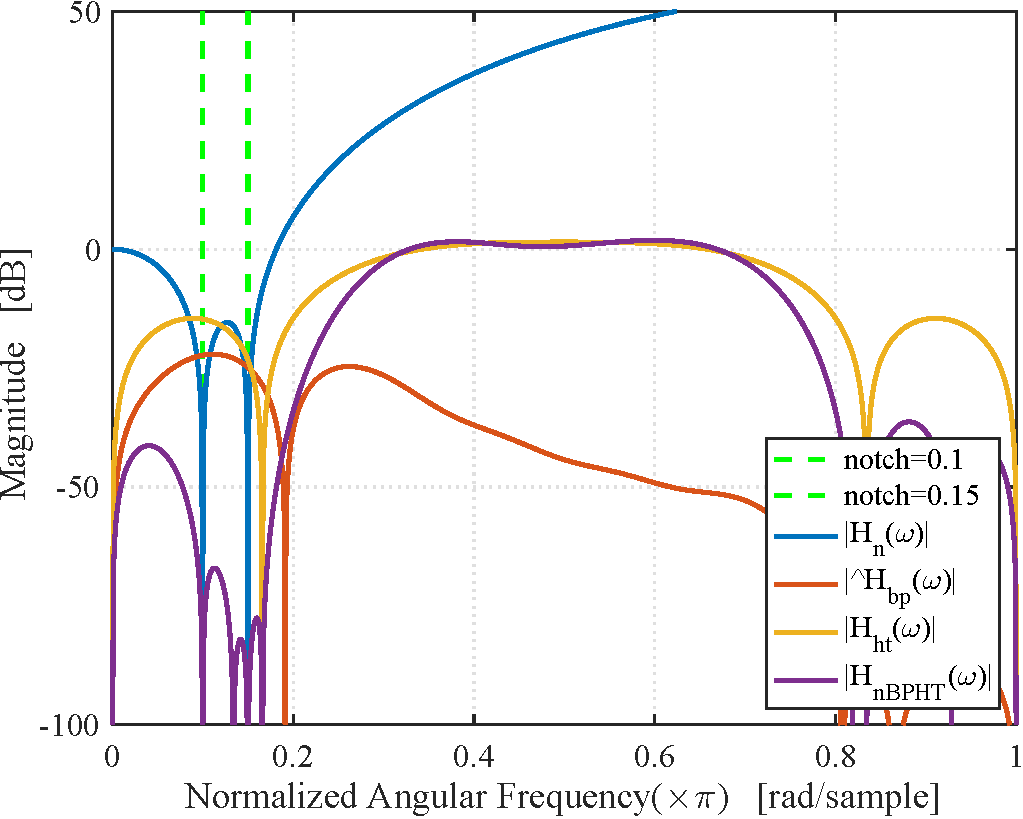
\includegraphics[width=8cm]
    		{Figure/figure01.pdf}
    \caption{のっちだおおおおおおお}
    \label{fig:man}
\end{figure}     <--第4章 まとめ
%#!platex main.tex
\chapter*{謝辞}
\addcontentsline{toc}{chapter}{謝辞} 
Other/thanks.texで文章を編集して下さい
%本研究にあたり,多大なるご指導とご助
%言を賜わりました.伊丹~ 誠教授,大野~光平先生に深く感謝いたします.また,色々
%な面でご協力いただいた伊丹研究室の大学院生の皆様,卒業研究生に対しまして
%も,心より感謝致します.最後に感謝の意を表して,本論文の謝辞とさせて頂きま
%す.

              <--謝辞
%#!platex main.tex
\chapter*{発表論文}
\addcontentsline{toc}{chapter}{発表論文}
\def\essection#1{\section*{#1}\addcontentsline{toc}{section}{#1}}

\essection{A.査読あり論文}
\begin{itemize}
\item Other/publicationで編集して下さい
\end{itemize}


\essection{B.国際会議}

\essection{C.研究会}

\essection{D.大会}

         <--発表論文リスト
\include{Other/bibliography}        <--参考文献
\end{verbatim}
です.
\begin{verbatim}
%#!platex main.tex
\chapter*{発表論文}
\addcontentsline{toc}{chapter}{発表論文}
\def\essection#1{\section*{#1}\addcontentsline{toc}{section}{#1}}

\essection{A.査読あり論文}
\begin{itemize}
\item Other/publicationで編集して下さい
\end{itemize}


\essection{B.国際会議}

\essection{C.研究会}

\essection{D.大会}


\end{verbatim}
は発表論文リストファイルですので卒論の場合,\verb|%|でコメントアウトして
 おいてください.

コンパイルの方法は

\framebox{\tt jlatex main.tex}

です.
しかし,これだけだと,目次が構成できないので,もう一度

\framebox{\tt jlatex main.tex}

とやると,目次も構成されます.
ちなみに,

\framebox{\tt make;make final}

とすると,main.psまではきます.
最後の最後の提出の時まではあまり使わないと思います.
修論などで,100ページ以上になると,psファイルがかなりでかくなるので,
 quotaに気をつけてください.
あと

\framebox{\tt make clean}

とすると,ディレクトリ内の掃除ができるのたまにやってもいいかも知れません.

また,yatexを利用すると,圧倒的に効率が良くなります.
この時,各LaTeXファイルに
\begin{verbatim}
%#!jlatex main.tex	
\end{verbatim}
という一行を加えておくと,どのLaTeXファイルからでもmain.texが呼べるので,
現在作業中のLaTeXファイル上で,jlatex main.texができます.
これはかなり便利です.
\section{おまけ}
図や表の引用で\verb|\ref|を利用すると思いますが,このスタイルでは
\verb|\ref{ラベル名}|とすると自動的に{\gt 図 {\bf 1}}のように出力するよ
うになっています.
これは表の引用,本文の引用においても同様です.
これが嫌な人はitlbthesis2012.styの最後の
\begin{verbatim}
\def\p@chapter{{\dg 本文}}
\def\p@section{{\dg 本文}}
\def\p@subsection{{\dg 本文}}
\def\p@subsubsection{{\dg 本文}}
\def\p@figure{{\dg 図}}
\def\p@table{{\dg 表}}
\let\origref=\ref
\def\ref#1{{\bf \origref{#1}}}
\end{verbatim}
を削除してください.



\include{Figure/figure}
%#!platex main.tex
\chapter{序論}

\section{章タイトル}
参考文献のテスト\cite{樋口龍雄2000}.
"bibliography.bib"の中身をいじると変更できます.

あいうえおかきくけこ
正弦波の周波数推定はレーダーやソナー,通信,医療などの領域で幅広く研究されてきた課題である\cite{R.G.McKilliam,K.Wang,D.Rife}.
一般に,単一正弦波に対する周波数推定を行う場合,アナログ信号であれば周波数カウンタを用いる手法,ディジタル信号の場合,相関を用いた手法やヒルベルト変換器を用いる手法が提案されている.
周波数カウンタを用いた手法では,1周期に対して基準クロックを用いて測定し,その逆数から周波数を求めるレシプロカル方式の周波数カウンタが知られている.しかしこの手法を用いる場合,周波数が変化すると出力間隔が不等間隔になる.そのため,計測値に対して,ディジタル処理を行う場合には補完処理などの工夫が必要となるため,サンプルごとに周波数の推定値が出力されるヒルベルト変換器を用いた手法が提案されている.\\
 ヒルベルト変換器を用いた手法では,入力を実部,出力を虚部とする複素信号の一種である解析信号の位相を時間微分し,瞬時角周波数から瞬時周波数を推定することができる.従来,ヒルベルト変換器は有限次数のFIRフィルタとして設計されるため振幅特性にリプルが生じ,出力は振動する場合がある.高尾ら\cite{高尾可変なし,高尾可変あり}は振動成分の周波数が入力周波数の偶数倍であることを理論的に示し,これを伝送零点を有する可変FIRフィルタを用いて振動成分を除去することで,低次数なヒルベルト変換器を用いても,単一正弦波の高精度な瞬時周波数推定が可能となることを示した.
%高尾さんのやつと関連させてノイズを取れることを書きたいなら,どういうノイズが取れて,どういうノイズがダメなのか明記する必要がある.
しかし実際にはノイズを含む信号を解析する必要がある.一般に,ノイズを含む信号に対して,ヒルベルト変換を行うためには,あらかじめ帯域通過フィルタによりノイズを低減させた後に,ヒルベルト変換器を縦続接続する方法が考えられる.しかし,帯域通過フィルタとヒルベルト変換器を1つのフィルタとして見た場合,全体の次数が増加し,結果として遅延や回路規模の増大につながり好ましくない.\\
 そこで本稿では,阻止域を有するヒルベルト変換器に対し,指定した位置に伝送零点を置くことで,ノイズを除去しながらヒルベルト変換可能なフィルタを設計する.阻止域を有するヒルベルト変換器を設計する場合,本来であれば阻止域において十分な減衰量を確保するために多くのフィルタ次数が必要となる.しかし,特定の周波数成分にノイズが含まれることがわかっている場合,その周波数成分のみに伝送零点を入れることにより,特定のノイズのみ除去しながらヒルベルト変換を行うことができ,減衰量を確保するために必要な次数を削減することができる.
最後に設計例を示し,提案法の有効性を確認する.
\section{指定した位置に伝送零点を有するヒルベルト変換器}
本章では提案するフィルタの設計問題について記す.提案するフィルタは,阻止域の指定した位置に伝送零点を有するヒルベルト変換器である.本稿で設計するフィルタの振幅理想特性を図\ref{ideal_resp}に示す.またフィルタの振幅理想特性は正規化角周波数$\omega$を用いて,

\begin{figure}[tb]
    \centering
    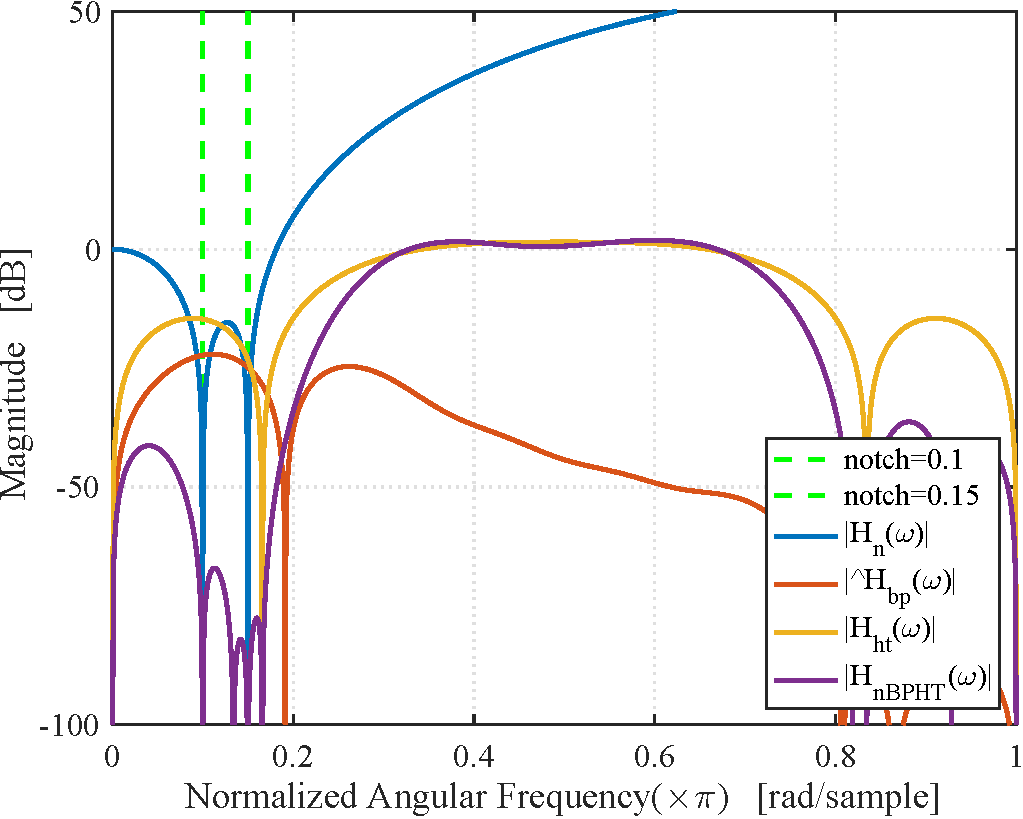
\includegraphics[width=8cm]
    		{Figure/figure01.pdf}
    \caption{のっちだおおおおおおお}
    \label{fig:man}
\end{figure}
%#!platex main.tex
\chapter*{謝辞}
\addcontentsline{toc}{chapter}{謝辞} 
Other/thanks.texで文章を編集して下さい
%本研究にあたり,多大なるご指導とご助
%言を賜わりました.伊丹~ 誠教授,大野~光平先生に深く感謝いたします.また,色々
%な面でご協力いただいた伊丹研究室の大学院生の皆様,卒業研究生に対しまして
%も,心より感謝致します.最後に感謝の意を表して,本論文の謝辞とさせて頂きま
%す.


\include{Other/bibliography}
%#!platex main.tex
\chapter*{発表論文}
\addcontentsline{toc}{chapter}{発表論文}
\def\essection#1{\section*{#1}\addcontentsline{toc}{section}{#1}}

\essection{A.査読あり論文}
\begin{itemize}
\item Other/publicationで編集して下さい
\end{itemize}


\essection{B.国際会議}

\essection{C.研究会}

\essection{D.大会}


\end{document}
\end{verbatim}
のようになっています.

\begin{verbatim}
\documentstyle[12pt,eclepsf,itlbthesis2000,eclclass]{j-report}
\end{verbatim}
でeclclassは\ref{itlbthesis2000ディレクトリ構成}を書くために必要なだけ
です.
ちなみにeclclass.styは\ref{itlbthesis2000ディレクトリ構成}のようなディ
レクトリ構造を書くのに便利なスタイルですが,使わなければ,
\begin{verbatim}
\documentstyle[12pt,eclepsf,itlbthesis2000]{j-report}
\end{verbatim}
としておいて結構です.
12pt.styは文字の大きさを指定するものではずさないでください.
またecleps.styはepsファイルを取り込むものなので,epsファイルを一枚も使わ
ない人ははずしても結構です(たぶんそんなことはない).
更に,スタイルファイル(例えばhere.sty)を追加する場合,
\begin{verbatim}
\documentstyle[12pt,eclepsf,itlbthesis2000,here]{j-report}
\end{verbatim}
のようにすればOKです.

\begin{verbatim}
\begin{document}
\itlbtitle    <---表紙を作ってます
\makeabstract <---アブストラクトを作ってます
\makecontents <---目次を作ってます
\end{verbatim}
は変更しないでください.

\begin{verbatim}
\include{}	
\end{verbatim}
は異なるLaTeXソースをincludeするもので,各章毎に別々のディレクトリで文章を
作ってください.

このようにする理由は次章で述べられているので,次の章は必ず読んでください.

従って,main.texで書き換える必要があるのは
\begin{verbatim}
\include{Introduction/introduction} <--第1章 序論
%#!platex main.tex

\chapter{このスタイルの使い方}
\section{このスタイルファイルについて}
このスタイルファイルの原型は1998年に修士を修了した下村さんが作成したもの
です.
それに初期設定ファイル等を加えて,LaTeXのマクロをブラックボックス化し,
あまりLaTeXのスタイルをわからない人でも使いやすいようにしたつもりです.
本来の目的は,PDF化に際しての編集者の負荷軽減の目的ですが,それほど難し
いスタイルではないので,解析して自分用に書き換えてもらっても結構です.
また,YaTeXを利用する事を前提にして作っている部分もあるので,なじみにく
い人は,過去のスタイルを利用するか,YaTeXを覚えてください.\\
\\
2012.11.20\\
itlbthesis2000.sty(j-tex用)をplatex用に改良したitlbthesis2012.styを作成しました.\\
以下の文章はitlbthesis2000の時のものとなっているので,注意して下さい.
また,バックアップを/home/yakou/Public/Styleの中に保存しておくので,何かありましたら参照してください.
\\
\section{ファイル構成}
まず,

\framebox{\tt gzip -d itlbthesis2000.tar.gz}

とし,

\framebox{\tt tar xvf itlbthesis2000.tar}

とすると,itlbthesis2000というディレクトリができると思います.

\framebox{\tt cd itlbthesis2000}

で中に入ると,その中身は\ref{itlbthesis2000ディレクトリ構成}のようになっ
ています.

ここで,とりあえず,

\framebox{\tt jlatex main.tex}

\framebox{\tt jlatex main.tex}

と2回jlatexをmain.texに対してかけてください.
そこにmain.dviがあるので,

\framebox{\tt xdvi-gs main.dvi}

とすると,このDVIファイルを見ることができます.
\section{設定の方法}
\begin{figure}[htb]
 \begin{center}
  \begin{classify}{\fbox{itlbthesis2000}\hspace*{5cm} $\circ$は全員必須,
   $*$は修士論文のみ必須}
   \class{
   \begin{classify}{\fbox{Introduction}(第1章)}
    \class{introduction.tex(第1章の\LaTeX ソース)}
   \end{classify}
   }
   \class{
   \begin{classify}{\fbox{StyleManual}第2章)}
    \class{stylemanual.tex(第2章の\LaTeX ソース)}
   \end{classify}
   }
   \class{
   \begin{classify}{\fbox{Figure}(第3章)}
    \class{
    \begin{classify}{\fbox{EPS}(第3章用EPSディレクトリ)}
     \class{hogehoge.eps(第3章に関するeps)}
    \end{classify}
    }
    \class{
    \begin{classify}{\fbox{XVD}(第3章用XVDディレクトリ)}
     \class{hogehoge.xvd(第3章に関するxvd)}
    \end{classify}
    }
    \class{figure.tex(第3章の\LaTeX ソース)}
   \end{classify}
   }
   \class{
   \begin{classify}{\fbox{Conclusion}(第4章)}
    \class{conclusion.tex(第4章に関する\LaTeX ソース)}
   \end{classify}
   }
   \class{
   \begin{classify}{\fbox{Other}(その他)}
    \class{abstract.tex(和文アブストラクト$)^{\circ}$}
    \class{abstract\_e.tex(英文アブストラクト$)^{*}$}
    \class{bibliography.tex(参考文献$)^{\circ}$}
    \class{publication.tex(発表論文$)^{*}$}
    \class{thanks.tex(謝辞$)^{\circ}$}
  \end{classify}
   }
   \class{Makefile(メイクファイル$)^{\circ}$}
   \class{eclclass.sty(この絵を書くためのだけのスタイル)}
   \class{init\_thesis.sty(初期設定ファイル$)^{\circ}$}
   \class{itlbthesis2000.sty(メインスタイルファイル$)^{\circ}$}
   \class{main.tex(メイン\LaTeX ソース$)^{\circ}$}
   \class{refcheck.sty(参照チェックスタイル)}
  \end{classify}
 \end{center}
 \caption{itlbthesis2000ディレクトリ構成}
 \label{itlbthesis2000ディレクトリ構成}
\end{figure}
\ref{itlbthesis2000ディレクトリ構成}を見てください.
この中で,itlbthesis2000.styはいじらなくても良いです.
\subsection{init\_thesis.styの書き方}
init\_thesis.styファイルは,初期設定ファイルです.中身は
\begin{verbatim}
%卒業論文の場合   \bm{卒業}
%修士論文の場合   \bm{修士}
\bm{修士}
%伊藤研究室の場合   \lab{伊藤}
%伊丹研究室の場合   \lab{伊丹}
\lab{伊藤}
%西暦の年   \year{}
\year{2001}
%平成の年   \heisei{}
\heisei{12}
%提出する月 \month{}
\month{2}
%論文の和文メインタイトル   \title{}
\title{卒業論文,修士論文の書き方}
%論文の英文メインタイトル(修論のみ)   \titleE{}
%卒論は空欄でOK
\titleE{How to draw up a bachelor's and master's thesis for our laboratory}
%論文の和文サブタイトル   \subtitle{}
%特になければ空欄でもOK 
\subtitle{サブタイトル}
%論文の英文サブタイトル(修論のみ)   \subtitleE{}
%特になければ空欄でもOK
%卒論は空欄でOK
\subtitleE{English sub-title}
%自分の学籍番号   \num{}
\num{8100701}
%自分の日本語の名前   \author{}
\author{藤井 雅弘}
%自分の英語の名前(修論のみ)   \authorE{}
%卒論は空欄でOK
\authorE{Masahiro Fujii}
%和文アブストラクトファイルの指定   \abstract{}
\abstract{Other/abstract.tex}	
%英文アブストラクトファイルの指定(修論のみ)   \abstractE{}
%卒論は空欄でOK
\abstruatE{Other/abstract_e.tex}	
\end{verbatim}
となってきます.
自分で勝手に書き換えてください.

卒論生は''修論のみ''となっている所はそのままでも,空欄でも結構です.
但し,コメントアウトしたり,その行自体を削除したりするとえらいことになり
ます.
一番上の\verb|\bm|を\verb|\bm{卒業}|としておけば,修論のみとなっている所
は反映されません.
\subsection{main.texの書き方}
このmain.dviのTeXソースmain.texは
\begin{verbatim}
\documentstyle[12pt,eclepsf,itlbthesis2000,eclclass]{j-report}
\begin{document}
\itlbtitle
\makeabstract
\makecontents
\include{Introduction/introduction}
%#!platex main.tex

\chapter{このスタイルの使い方}
\section{このスタイルファイルについて}
このスタイルファイルの原型は1998年に修士を修了した下村さんが作成したもの
です.
それに初期設定ファイル等を加えて,LaTeXのマクロをブラックボックス化し,
あまりLaTeXのスタイルをわからない人でも使いやすいようにしたつもりです.
本来の目的は,PDF化に際しての編集者の負荷軽減の目的ですが,それほど難し
いスタイルではないので,解析して自分用に書き換えてもらっても結構です.
また,YaTeXを利用する事を前提にして作っている部分もあるので,なじみにく
い人は,過去のスタイルを利用するか,YaTeXを覚えてください.\\
\\
2012.11.20\\
itlbthesis2000.sty(j-tex用)をplatex用に改良したitlbthesis2012.styを作成しました.\\
以下の文章はitlbthesis2000の時のものとなっているので,注意して下さい.
また,バックアップを/home/yakou/Public/Styleの中に保存しておくので,何かありましたら参照してください.
\\
\section{ファイル構成}
まず,

\framebox{\tt gzip -d itlbthesis2000.tar.gz}

とし,

\framebox{\tt tar xvf itlbthesis2000.tar}

とすると,itlbthesis2000というディレクトリができると思います.

\framebox{\tt cd itlbthesis2000}

で中に入ると,その中身は\ref{itlbthesis2000ディレクトリ構成}のようになっ
ています.

ここで,とりあえず,

\framebox{\tt jlatex main.tex}

\framebox{\tt jlatex main.tex}

と2回jlatexをmain.texに対してかけてください.
そこにmain.dviがあるので,

\framebox{\tt xdvi-gs main.dvi}

とすると,このDVIファイルを見ることができます.
\section{設定の方法}
\begin{figure}[htb]
 \begin{center}
  \begin{classify}{\fbox{itlbthesis2000}\hspace*{5cm} $\circ$は全員必須,
   $*$は修士論文のみ必須}
   \class{
   \begin{classify}{\fbox{Introduction}(第1章)}
    \class{introduction.tex(第1章の\LaTeX ソース)}
   \end{classify}
   }
   \class{
   \begin{classify}{\fbox{StyleManual}第2章)}
    \class{stylemanual.tex(第2章の\LaTeX ソース)}
   \end{classify}
   }
   \class{
   \begin{classify}{\fbox{Figure}(第3章)}
    \class{
    \begin{classify}{\fbox{EPS}(第3章用EPSディレクトリ)}
     \class{hogehoge.eps(第3章に関するeps)}
    \end{classify}
    }
    \class{
    \begin{classify}{\fbox{XVD}(第3章用XVDディレクトリ)}
     \class{hogehoge.xvd(第3章に関するxvd)}
    \end{classify}
    }
    \class{figure.tex(第3章の\LaTeX ソース)}
   \end{classify}
   }
   \class{
   \begin{classify}{\fbox{Conclusion}(第4章)}
    \class{conclusion.tex(第4章に関する\LaTeX ソース)}
   \end{classify}
   }
   \class{
   \begin{classify}{\fbox{Other}(その他)}
    \class{abstract.tex(和文アブストラクト$)^{\circ}$}
    \class{abstract\_e.tex(英文アブストラクト$)^{*}$}
    \class{bibliography.tex(参考文献$)^{\circ}$}
    \class{publication.tex(発表論文$)^{*}$}
    \class{thanks.tex(謝辞$)^{\circ}$}
  \end{classify}
   }
   \class{Makefile(メイクファイル$)^{\circ}$}
   \class{eclclass.sty(この絵を書くためのだけのスタイル)}
   \class{init\_thesis.sty(初期設定ファイル$)^{\circ}$}
   \class{itlbthesis2000.sty(メインスタイルファイル$)^{\circ}$}
   \class{main.tex(メイン\LaTeX ソース$)^{\circ}$}
   \class{refcheck.sty(参照チェックスタイル)}
  \end{classify}
 \end{center}
 \caption{itlbthesis2000ディレクトリ構成}
 \label{itlbthesis2000ディレクトリ構成}
\end{figure}
\ref{itlbthesis2000ディレクトリ構成}を見てください.
この中で,itlbthesis2000.styはいじらなくても良いです.
\subsection{init\_thesis.styの書き方}
init\_thesis.styファイルは,初期設定ファイルです.中身は
\begin{verbatim}
%卒業論文の場合   \bm{卒業}
%修士論文の場合   \bm{修士}
\bm{修士}
%伊藤研究室の場合   \lab{伊藤}
%伊丹研究室の場合   \lab{伊丹}
\lab{伊藤}
%西暦の年   \year{}
\year{2001}
%平成の年   \heisei{}
\heisei{12}
%提出する月 \month{}
\month{2}
%論文の和文メインタイトル   \title{}
\title{卒業論文,修士論文の書き方}
%論文の英文メインタイトル(修論のみ)   \titleE{}
%卒論は空欄でOK
\titleE{How to draw up a bachelor's and master's thesis for our laboratory}
%論文の和文サブタイトル   \subtitle{}
%特になければ空欄でもOK 
\subtitle{サブタイトル}
%論文の英文サブタイトル(修論のみ)   \subtitleE{}
%特になければ空欄でもOK
%卒論は空欄でOK
\subtitleE{English sub-title}
%自分の学籍番号   \num{}
\num{8100701}
%自分の日本語の名前   \author{}
\author{藤井 雅弘}
%自分の英語の名前(修論のみ)   \authorE{}
%卒論は空欄でOK
\authorE{Masahiro Fujii}
%和文アブストラクトファイルの指定   \abstract{}
\abstract{Other/abstract.tex}	
%英文アブストラクトファイルの指定(修論のみ)   \abstractE{}
%卒論は空欄でOK
\abstruatE{Other/abstract_e.tex}	
\end{verbatim}
となってきます.
自分で勝手に書き換えてください.

卒論生は''修論のみ''となっている所はそのままでも,空欄でも結構です.
但し,コメントアウトしたり,その行自体を削除したりするとえらいことになり
ます.
一番上の\verb|\bm|を\verb|\bm{卒業}|としておけば,修論のみとなっている所
は反映されません.
\subsection{main.texの書き方}
このmain.dviのTeXソースmain.texは
\begin{verbatim}
\documentstyle[12pt,eclepsf,itlbthesis2000,eclclass]{j-report}
\begin{document}
\itlbtitle
\makeabstract
\makecontents
\include{Introduction/introduction}
\include{StyleManual/stylemanual}
\include{Figure/figure}
\include{Conclusion/conclusion}
\include{Other/thanks}
\include{Other/bibliography}
\include{Other/publication}
\end{document}
\end{verbatim}
のようになっています.

\begin{verbatim}
\documentstyle[12pt,eclepsf,itlbthesis2000,eclclass]{j-report}
\end{verbatim}
でeclclassは\ref{itlbthesis2000ディレクトリ構成}を書くために必要なだけ
です.
ちなみにeclclass.styは\ref{itlbthesis2000ディレクトリ構成}のようなディ
レクトリ構造を書くのに便利なスタイルですが,使わなければ,
\begin{verbatim}
\documentstyle[12pt,eclepsf,itlbthesis2000]{j-report}
\end{verbatim}
としておいて結構です.
12pt.styは文字の大きさを指定するものではずさないでください.
またecleps.styはepsファイルを取り込むものなので,epsファイルを一枚も使わ
ない人ははずしても結構です(たぶんそんなことはない).
更に,スタイルファイル(例えばhere.sty)を追加する場合,
\begin{verbatim}
\documentstyle[12pt,eclepsf,itlbthesis2000,here]{j-report}
\end{verbatim}
のようにすればOKです.

\begin{verbatim}
\begin{document}
\itlbtitle    <---表紙を作ってます
\makeabstract <---アブストラクトを作ってます
\makecontents <---目次を作ってます
\end{verbatim}
は変更しないでください.

\begin{verbatim}
\include{}	
\end{verbatim}
は異なるLaTeXソースをincludeするもので,各章毎に別々のディレクトリで文章を
作ってください.

このようにする理由は次章で述べられているので,次の章は必ず読んでください.

従って,main.texで書き換える必要があるのは
\begin{verbatim}
\include{Introduction/introduction} <--第1章 序論
\include{StyleManual/stylemanual}   <--第2章 スタイルファイルの使い方
\include{Figure/figure}             <--第3章 絵の貼り方
\include{Conclusion/conclusion}     <--第4章 まとめ
\include{Other/thanks}              <--謝辞
\include{Other/publication}         <--発表論文リスト
\include{Other/bibliography}        <--参考文献
\end{verbatim}
です.
\begin{verbatim}
\include{Other/publication}
\end{verbatim}
は発表論文リストファイルですので卒論の場合,\verb|%|でコメントアウトして
 おいてください.

コンパイルの方法は

\framebox{\tt jlatex main.tex}

です.
しかし,これだけだと,目次が構成できないので,もう一度

\framebox{\tt jlatex main.tex}

とやると,目次も構成されます.
ちなみに,

\framebox{\tt make;make final}

とすると,main.psまではきます.
最後の最後の提出の時まではあまり使わないと思います.
修論などで,100ページ以上になると,psファイルがかなりでかくなるので,
 quotaに気をつけてください.
あと

\framebox{\tt make clean}

とすると,ディレクトリ内の掃除ができるのたまにやってもいいかも知れません.

また,yatexを利用すると,圧倒的に効率が良くなります.
この時,各LaTeXファイルに
\begin{verbatim}
%#!jlatex main.tex	
\end{verbatim}
という一行を加えておくと,どのLaTeXファイルからでもmain.texが呼べるので,
現在作業中のLaTeXファイル上で,jlatex main.texができます.
これはかなり便利です.
\section{おまけ}
図や表の引用で\verb|\ref|を利用すると思いますが,このスタイルでは
\verb|\ref{ラベル名}|とすると自動的に{\gt 図 {\bf 1}}のように出力するよ
うになっています.
これは表の引用,本文の引用においても同様です.
これが嫌な人はitlbthesis2012.styの最後の
\begin{verbatim}
\def\p@chapter{{\dg 本文}}
\def\p@section{{\dg 本文}}
\def\p@subsection{{\dg 本文}}
\def\p@subsubsection{{\dg 本文}}
\def\p@figure{{\dg 図}}
\def\p@table{{\dg 表}}
\let\origref=\ref
\def\ref#1{{\bf \origref{#1}}}
\end{verbatim}
を削除してください.



\include{Figure/figure}
%#!platex main.tex
\chapter{序論}

\section{章タイトル}
参考文献のテスト\cite{樋口龍雄2000}.
"bibliography.bib"の中身をいじると変更できます.

あいうえおかきくけこ
正弦波の周波数推定はレーダーやソナー,通信,医療などの領域で幅広く研究されてきた課題である\cite{R.G.McKilliam,K.Wang,D.Rife}.
一般に,単一正弦波に対する周波数推定を行う場合,アナログ信号であれば周波数カウンタを用いる手法,ディジタル信号の場合,相関を用いた手法やヒルベルト変換器を用いる手法が提案されている.
周波数カウンタを用いた手法では,1周期に対して基準クロックを用いて測定し,その逆数から周波数を求めるレシプロカル方式の周波数カウンタが知られている.しかしこの手法を用いる場合,周波数が変化すると出力間隔が不等間隔になる.そのため,計測値に対して,ディジタル処理を行う場合には補完処理などの工夫が必要となるため,サンプルごとに周波数の推定値が出力されるヒルベルト変換器を用いた手法が提案されている.\\
 ヒルベルト変換器を用いた手法では,入力を実部,出力を虚部とする複素信号の一種である解析信号の位相を時間微分し,瞬時角周波数から瞬時周波数を推定することができる.従来,ヒルベルト変換器は有限次数のFIRフィルタとして設計されるため振幅特性にリプルが生じ,出力は振動する場合がある.高尾ら\cite{高尾可変なし,高尾可変あり}は振動成分の周波数が入力周波数の偶数倍であることを理論的に示し,これを伝送零点を有する可変FIRフィルタを用いて振動成分を除去することで,低次数なヒルベルト変換器を用いても,単一正弦波の高精度な瞬時周波数推定が可能となることを示した.
%高尾さんのやつと関連させてノイズを取れることを書きたいなら,どういうノイズが取れて,どういうノイズがダメなのか明記する必要がある.
しかし実際にはノイズを含む信号を解析する必要がある.一般に,ノイズを含む信号に対して,ヒルベルト変換を行うためには,あらかじめ帯域通過フィルタによりノイズを低減させた後に,ヒルベルト変換器を縦続接続する方法が考えられる.しかし,帯域通過フィルタとヒルベルト変換器を1つのフィルタとして見た場合,全体の次数が増加し,結果として遅延や回路規模の増大につながり好ましくない.\\
 そこで本稿では,阻止域を有するヒルベルト変換器に対し,指定した位置に伝送零点を置くことで,ノイズを除去しながらヒルベルト変換可能なフィルタを設計する.阻止域を有するヒルベルト変換器を設計する場合,本来であれば阻止域において十分な減衰量を確保するために多くのフィルタ次数が必要となる.しかし,特定の周波数成分にノイズが含まれることがわかっている場合,その周波数成分のみに伝送零点を入れることにより,特定のノイズのみ除去しながらヒルベルト変換を行うことができ,減衰量を確保するために必要な次数を削減することができる.
最後に設計例を示し,提案法の有効性を確認する.
\section{指定した位置に伝送零点を有するヒルベルト変換器}
本章では提案するフィルタの設計問題について記す.提案するフィルタは,阻止域の指定した位置に伝送零点を有するヒルベルト変換器である.本稿で設計するフィルタの振幅理想特性を図\ref{ideal_resp}に示す.またフィルタの振幅理想特性は正規化角周波数$\omega$を用いて,

\begin{figure}[tb]
    \centering
    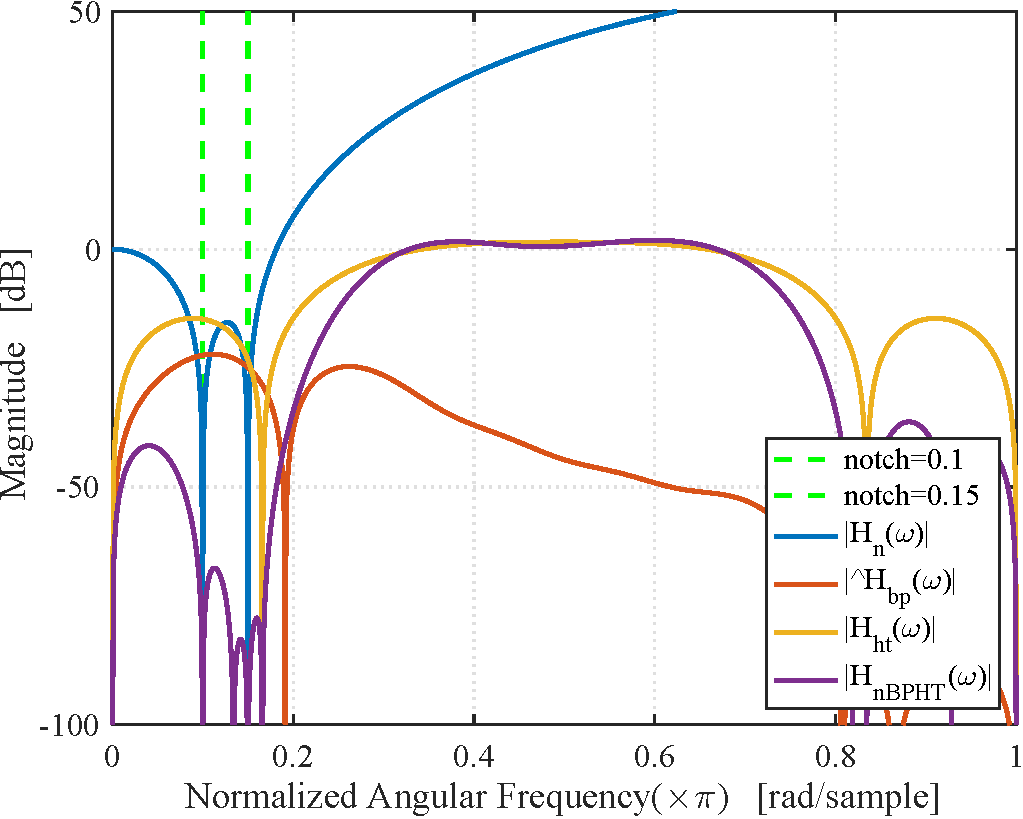
\includegraphics[width=8cm]
    		{Figure/figure01.pdf}
    \caption{のっちだおおおおおおお}
    \label{fig:man}
\end{figure}
%#!platex main.tex
\chapter*{謝辞}
\addcontentsline{toc}{chapter}{謝辞} 
Other/thanks.texで文章を編集して下さい
%本研究にあたり,多大なるご指導とご助
%言を賜わりました.伊丹~ 誠教授,大野~光平先生に深く感謝いたします.また,色々
%な面でご協力いただいた伊丹研究室の大学院生の皆様,卒業研究生に対しまして
%も,心より感謝致します.最後に感謝の意を表して,本論文の謝辞とさせて頂きま
%す.


\include{Other/bibliography}
%#!platex main.tex
\chapter*{発表論文}
\addcontentsline{toc}{chapter}{発表論文}
\def\essection#1{\section*{#1}\addcontentsline{toc}{section}{#1}}

\essection{A.査読あり論文}
\begin{itemize}
\item Other/publicationで編集して下さい
\end{itemize}


\essection{B.国際会議}

\essection{C.研究会}

\essection{D.大会}


\end{document}
\end{verbatim}
のようになっています.

\begin{verbatim}
\documentstyle[12pt,eclepsf,itlbthesis2000,eclclass]{j-report}
\end{verbatim}
でeclclassは\ref{itlbthesis2000ディレクトリ構成}を書くために必要なだけ
です.
ちなみにeclclass.styは\ref{itlbthesis2000ディレクトリ構成}のようなディ
レクトリ構造を書くのに便利なスタイルですが,使わなければ,
\begin{verbatim}
\documentstyle[12pt,eclepsf,itlbthesis2000]{j-report}
\end{verbatim}
としておいて結構です.
12pt.styは文字の大きさを指定するものではずさないでください.
またecleps.styはepsファイルを取り込むものなので,epsファイルを一枚も使わ
ない人ははずしても結構です(たぶんそんなことはない).
更に,スタイルファイル(例えばhere.sty)を追加する場合,
\begin{verbatim}
\documentstyle[12pt,eclepsf,itlbthesis2000,here]{j-report}
\end{verbatim}
のようにすればOKです.

\begin{verbatim}
\begin{document}
\itlbtitle    <---表紙を作ってます
\makeabstract <---アブストラクトを作ってます
\makecontents <---目次を作ってます
\end{verbatim}
は変更しないでください.

\begin{verbatim}
\include{}	
\end{verbatim}
は異なるLaTeXソースをincludeするもので,各章毎に別々のディレクトリで文章を
作ってください.

このようにする理由は次章で述べられているので,次の章は必ず読んでください.

従って,main.texで書き換える必要があるのは
\begin{verbatim}
\include{Introduction/introduction} <--第1章 序論
%#!platex main.tex

\chapter{このスタイルの使い方}
\section{このスタイルファイルについて}
このスタイルファイルの原型は1998年に修士を修了した下村さんが作成したもの
です.
それに初期設定ファイル等を加えて,LaTeXのマクロをブラックボックス化し,
あまりLaTeXのスタイルをわからない人でも使いやすいようにしたつもりです.
本来の目的は,PDF化に際しての編集者の負荷軽減の目的ですが,それほど難し
いスタイルではないので,解析して自分用に書き換えてもらっても結構です.
また,YaTeXを利用する事を前提にして作っている部分もあるので,なじみにく
い人は,過去のスタイルを利用するか,YaTeXを覚えてください.\\
\\
2012.11.20\\
itlbthesis2000.sty(j-tex用)をplatex用に改良したitlbthesis2012.styを作成しました.\\
以下の文章はitlbthesis2000の時のものとなっているので,注意して下さい.
また,バックアップを/home/yakou/Public/Styleの中に保存しておくので,何かありましたら参照してください.
\\
\section{ファイル構成}
まず,

\framebox{\tt gzip -d itlbthesis2000.tar.gz}

とし,

\framebox{\tt tar xvf itlbthesis2000.tar}

とすると,itlbthesis2000というディレクトリができると思います.

\framebox{\tt cd itlbthesis2000}

で中に入ると,その中身は\ref{itlbthesis2000ディレクトリ構成}のようになっ
ています.

ここで,とりあえず,

\framebox{\tt jlatex main.tex}

\framebox{\tt jlatex main.tex}

と2回jlatexをmain.texに対してかけてください.
そこにmain.dviがあるので,

\framebox{\tt xdvi-gs main.dvi}

とすると,このDVIファイルを見ることができます.
\section{設定の方法}
\begin{figure}[htb]
 \begin{center}
  \begin{classify}{\fbox{itlbthesis2000}\hspace*{5cm} $\circ$は全員必須,
   $*$は修士論文のみ必須}
   \class{
   \begin{classify}{\fbox{Introduction}(第1章)}
    \class{introduction.tex(第1章の\LaTeX ソース)}
   \end{classify}
   }
   \class{
   \begin{classify}{\fbox{StyleManual}第2章)}
    \class{stylemanual.tex(第2章の\LaTeX ソース)}
   \end{classify}
   }
   \class{
   \begin{classify}{\fbox{Figure}(第3章)}
    \class{
    \begin{classify}{\fbox{EPS}(第3章用EPSディレクトリ)}
     \class{hogehoge.eps(第3章に関するeps)}
    \end{classify}
    }
    \class{
    \begin{classify}{\fbox{XVD}(第3章用XVDディレクトリ)}
     \class{hogehoge.xvd(第3章に関するxvd)}
    \end{classify}
    }
    \class{figure.tex(第3章の\LaTeX ソース)}
   \end{classify}
   }
   \class{
   \begin{classify}{\fbox{Conclusion}(第4章)}
    \class{conclusion.tex(第4章に関する\LaTeX ソース)}
   \end{classify}
   }
   \class{
   \begin{classify}{\fbox{Other}(その他)}
    \class{abstract.tex(和文アブストラクト$)^{\circ}$}
    \class{abstract\_e.tex(英文アブストラクト$)^{*}$}
    \class{bibliography.tex(参考文献$)^{\circ}$}
    \class{publication.tex(発表論文$)^{*}$}
    \class{thanks.tex(謝辞$)^{\circ}$}
  \end{classify}
   }
   \class{Makefile(メイクファイル$)^{\circ}$}
   \class{eclclass.sty(この絵を書くためのだけのスタイル)}
   \class{init\_thesis.sty(初期設定ファイル$)^{\circ}$}
   \class{itlbthesis2000.sty(メインスタイルファイル$)^{\circ}$}
   \class{main.tex(メイン\LaTeX ソース$)^{\circ}$}
   \class{refcheck.sty(参照チェックスタイル)}
  \end{classify}
 \end{center}
 \caption{itlbthesis2000ディレクトリ構成}
 \label{itlbthesis2000ディレクトリ構成}
\end{figure}
\ref{itlbthesis2000ディレクトリ構成}を見てください.
この中で,itlbthesis2000.styはいじらなくても良いです.
\subsection{init\_thesis.styの書き方}
init\_thesis.styファイルは,初期設定ファイルです.中身は
\begin{verbatim}
%卒業論文の場合   \bm{卒業}
%修士論文の場合   \bm{修士}
\bm{修士}
%伊藤研究室の場合   \lab{伊藤}
%伊丹研究室の場合   \lab{伊丹}
\lab{伊藤}
%西暦の年   \year{}
\year{2001}
%平成の年   \heisei{}
\heisei{12}
%提出する月 \month{}
\month{2}
%論文の和文メインタイトル   \title{}
\title{卒業論文,修士論文の書き方}
%論文の英文メインタイトル(修論のみ)   \titleE{}
%卒論は空欄でOK
\titleE{How to draw up a bachelor's and master's thesis for our laboratory}
%論文の和文サブタイトル   \subtitle{}
%特になければ空欄でもOK 
\subtitle{サブタイトル}
%論文の英文サブタイトル(修論のみ)   \subtitleE{}
%特になければ空欄でもOK
%卒論は空欄でOK
\subtitleE{English sub-title}
%自分の学籍番号   \num{}
\num{8100701}
%自分の日本語の名前   \author{}
\author{藤井 雅弘}
%自分の英語の名前(修論のみ)   \authorE{}
%卒論は空欄でOK
\authorE{Masahiro Fujii}
%和文アブストラクトファイルの指定   \abstract{}
\abstract{Other/abstract.tex}	
%英文アブストラクトファイルの指定(修論のみ)   \abstractE{}
%卒論は空欄でOK
\abstruatE{Other/abstract_e.tex}	
\end{verbatim}
となってきます.
自分で勝手に書き換えてください.

卒論生は''修論のみ''となっている所はそのままでも,空欄でも結構です.
但し,コメントアウトしたり,その行自体を削除したりするとえらいことになり
ます.
一番上の\verb|\bm|を\verb|\bm{卒業}|としておけば,修論のみとなっている所
は反映されません.
\subsection{main.texの書き方}
このmain.dviのTeXソースmain.texは
\begin{verbatim}
\documentstyle[12pt,eclepsf,itlbthesis2000,eclclass]{j-report}
\begin{document}
\itlbtitle
\makeabstract
\makecontents
\include{Introduction/introduction}
\include{StyleManual/stylemanual}
\include{Figure/figure}
\include{Conclusion/conclusion}
\include{Other/thanks}
\include{Other/bibliography}
\include{Other/publication}
\end{document}
\end{verbatim}
のようになっています.

\begin{verbatim}
\documentstyle[12pt,eclepsf,itlbthesis2000,eclclass]{j-report}
\end{verbatim}
でeclclassは\ref{itlbthesis2000ディレクトリ構成}を書くために必要なだけ
です.
ちなみにeclclass.styは\ref{itlbthesis2000ディレクトリ構成}のようなディ
レクトリ構造を書くのに便利なスタイルですが,使わなければ,
\begin{verbatim}
\documentstyle[12pt,eclepsf,itlbthesis2000]{j-report}
\end{verbatim}
としておいて結構です.
12pt.styは文字の大きさを指定するものではずさないでください.
またecleps.styはepsファイルを取り込むものなので,epsファイルを一枚も使わ
ない人ははずしても結構です(たぶんそんなことはない).
更に,スタイルファイル(例えばhere.sty)を追加する場合,
\begin{verbatim}
\documentstyle[12pt,eclepsf,itlbthesis2000,here]{j-report}
\end{verbatim}
のようにすればOKです.

\begin{verbatim}
\begin{document}
\itlbtitle    <---表紙を作ってます
\makeabstract <---アブストラクトを作ってます
\makecontents <---目次を作ってます
\end{verbatim}
は変更しないでください.

\begin{verbatim}
\include{}	
\end{verbatim}
は異なるLaTeXソースをincludeするもので,各章毎に別々のディレクトリで文章を
作ってください.

このようにする理由は次章で述べられているので,次の章は必ず読んでください.

従って,main.texで書き換える必要があるのは
\begin{verbatim}
\include{Introduction/introduction} <--第1章 序論
\include{StyleManual/stylemanual}   <--第2章 スタイルファイルの使い方
\include{Figure/figure}             <--第3章 絵の貼り方
\include{Conclusion/conclusion}     <--第4章 まとめ
\include{Other/thanks}              <--謝辞
\include{Other/publication}         <--発表論文リスト
\include{Other/bibliography}        <--参考文献
\end{verbatim}
です.
\begin{verbatim}
\include{Other/publication}
\end{verbatim}
は発表論文リストファイルですので卒論の場合,\verb|%|でコメントアウトして
 おいてください.

コンパイルの方法は

\framebox{\tt jlatex main.tex}

です.
しかし,これだけだと,目次が構成できないので,もう一度

\framebox{\tt jlatex main.tex}

とやると,目次も構成されます.
ちなみに,

\framebox{\tt make;make final}

とすると,main.psまではきます.
最後の最後の提出の時まではあまり使わないと思います.
修論などで,100ページ以上になると,psファイルがかなりでかくなるので,
 quotaに気をつけてください.
あと

\framebox{\tt make clean}

とすると,ディレクトリ内の掃除ができるのたまにやってもいいかも知れません.

また,yatexを利用すると,圧倒的に効率が良くなります.
この時,各LaTeXファイルに
\begin{verbatim}
%#!jlatex main.tex	
\end{verbatim}
という一行を加えておくと,どのLaTeXファイルからでもmain.texが呼べるので,
現在作業中のLaTeXファイル上で,jlatex main.texができます.
これはかなり便利です.
\section{おまけ}
図や表の引用で\verb|\ref|を利用すると思いますが,このスタイルでは
\verb|\ref{ラベル名}|とすると自動的に{\gt 図 {\bf 1}}のように出力するよ
うになっています.
これは表の引用,本文の引用においても同様です.
これが嫌な人はitlbthesis2012.styの最後の
\begin{verbatim}
\def\p@chapter{{\dg 本文}}
\def\p@section{{\dg 本文}}
\def\p@subsection{{\dg 本文}}
\def\p@subsubsection{{\dg 本文}}
\def\p@figure{{\dg 図}}
\def\p@table{{\dg 表}}
\let\origref=\ref
\def\ref#1{{\bf \origref{#1}}}
\end{verbatim}
を削除してください.


   <--第2章 スタイルファイルの使い方
\include{Figure/figure}             <--第3章 絵の貼り方
%#!platex main.tex
\chapter{序論}

\section{章タイトル}
参考文献のテスト\cite{樋口龍雄2000}.
"bibliography.bib"の中身をいじると変更できます.

あいうえおかきくけこ
正弦波の周波数推定はレーダーやソナー,通信,医療などの領域で幅広く研究されてきた課題である\cite{R.G.McKilliam,K.Wang,D.Rife}.
一般に,単一正弦波に対する周波数推定を行う場合,アナログ信号であれば周波数カウンタを用いる手法,ディジタル信号の場合,相関を用いた手法やヒルベルト変換器を用いる手法が提案されている.
周波数カウンタを用いた手法では,1周期に対して基準クロックを用いて測定し,その逆数から周波数を求めるレシプロカル方式の周波数カウンタが知られている.しかしこの手法を用いる場合,周波数が変化すると出力間隔が不等間隔になる.そのため,計測値に対して,ディジタル処理を行う場合には補完処理などの工夫が必要となるため,サンプルごとに周波数の推定値が出力されるヒルベルト変換器を用いた手法が提案されている.\\
 ヒルベルト変換器を用いた手法では,入力を実部,出力を虚部とする複素信号の一種である解析信号の位相を時間微分し,瞬時角周波数から瞬時周波数を推定することができる.従来,ヒルベルト変換器は有限次数のFIRフィルタとして設計されるため振幅特性にリプルが生じ,出力は振動する場合がある.高尾ら\cite{高尾可変なし,高尾可変あり}は振動成分の周波数が入力周波数の偶数倍であることを理論的に示し,これを伝送零点を有する可変FIRフィルタを用いて振動成分を除去することで,低次数なヒルベルト変換器を用いても,単一正弦波の高精度な瞬時周波数推定が可能となることを示した.
%高尾さんのやつと関連させてノイズを取れることを書きたいなら,どういうノイズが取れて,どういうノイズがダメなのか明記する必要がある.
しかし実際にはノイズを含む信号を解析する必要がある.一般に,ノイズを含む信号に対して,ヒルベルト変換を行うためには,あらかじめ帯域通過フィルタによりノイズを低減させた後に,ヒルベルト変換器を縦続接続する方法が考えられる.しかし,帯域通過フィルタとヒルベルト変換器を1つのフィルタとして見た場合,全体の次数が増加し,結果として遅延や回路規模の増大につながり好ましくない.\\
 そこで本稿では,阻止域を有するヒルベルト変換器に対し,指定した位置に伝送零点を置くことで,ノイズを除去しながらヒルベルト変換可能なフィルタを設計する.阻止域を有するヒルベルト変換器を設計する場合,本来であれば阻止域において十分な減衰量を確保するために多くのフィルタ次数が必要となる.しかし,特定の周波数成分にノイズが含まれることがわかっている場合,その周波数成分のみに伝送零点を入れることにより,特定のノイズのみ除去しながらヒルベルト変換を行うことができ,減衰量を確保するために必要な次数を削減することができる.
最後に設計例を示し,提案法の有効性を確認する.
\section{指定した位置に伝送零点を有するヒルベルト変換器}
本章では提案するフィルタの設計問題について記す.提案するフィルタは,阻止域の指定した位置に伝送零点を有するヒルベルト変換器である.本稿で設計するフィルタの振幅理想特性を図\ref{ideal_resp}に示す.またフィルタの振幅理想特性は正規化角周波数$\omega$を用いて,

\begin{figure}[tb]
    \centering
    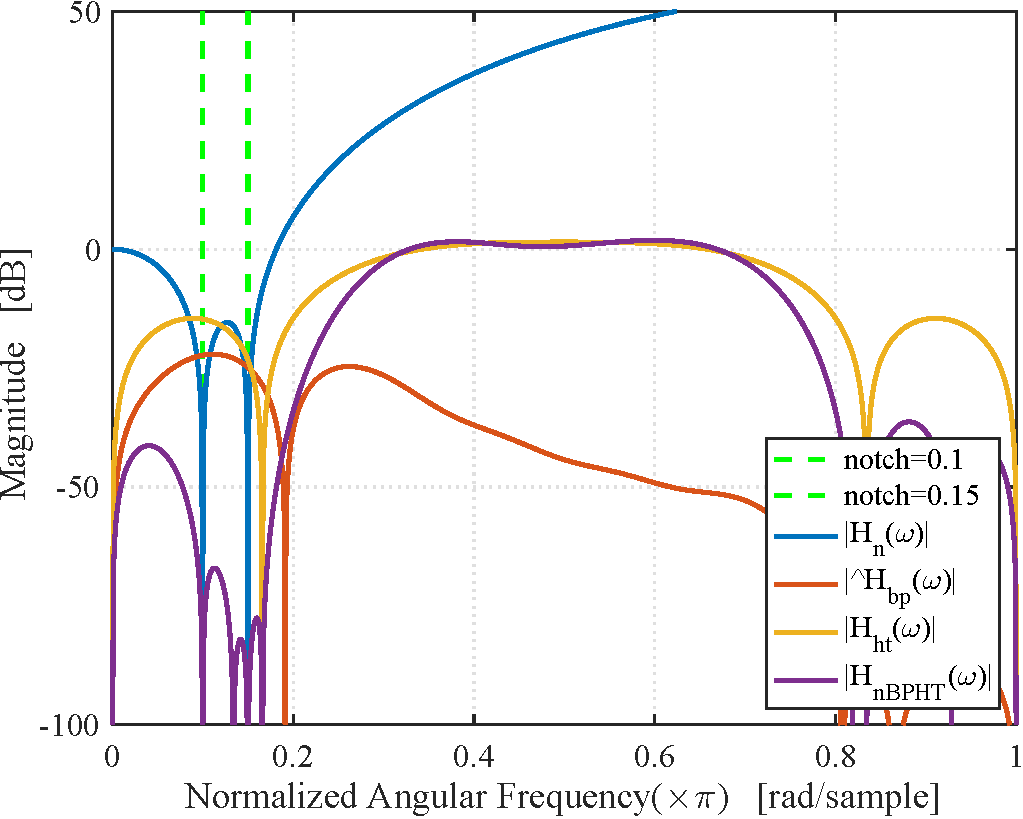
\includegraphics[width=8cm]
    		{Figure/figure01.pdf}
    \caption{のっちだおおおおおおお}
    \label{fig:man}
\end{figure}     <--第4章 まとめ
%#!platex main.tex
\chapter*{謝辞}
\addcontentsline{toc}{chapter}{謝辞} 
Other/thanks.texで文章を編集して下さい
%本研究にあたり,多大なるご指導とご助
%言を賜わりました.伊丹~ 誠教授,大野~光平先生に深く感謝いたします.また,色々
%な面でご協力いただいた伊丹研究室の大学院生の皆様,卒業研究生に対しまして
%も,心より感謝致します.最後に感謝の意を表して,本論文の謝辞とさせて頂きま
%す.

              <--謝辞
%#!platex main.tex
\chapter*{発表論文}
\addcontentsline{toc}{chapter}{発表論文}
\def\essection#1{\section*{#1}\addcontentsline{toc}{section}{#1}}

\essection{A.査読あり論文}
\begin{itemize}
\item Other/publicationで編集して下さい
\end{itemize}


\essection{B.国際会議}

\essection{C.研究会}

\essection{D.大会}

         <--発表論文リスト
\include{Other/bibliography}        <--参考文献
\end{verbatim}
です.
\begin{verbatim}
%#!platex main.tex
\chapter*{発表論文}
\addcontentsline{toc}{chapter}{発表論文}
\def\essection#1{\section*{#1}\addcontentsline{toc}{section}{#1}}

\essection{A.査読あり論文}
\begin{itemize}
\item Other/publicationで編集して下さい
\end{itemize}


\essection{B.国際会議}

\essection{C.研究会}

\essection{D.大会}


\end{verbatim}
は発表論文リストファイルですので卒論の場合,\verb|%|でコメントアウトして
 おいてください.

コンパイルの方法は

\framebox{\tt jlatex main.tex}

です.
しかし,これだけだと,目次が構成できないので,もう一度

\framebox{\tt jlatex main.tex}

とやると,目次も構成されます.
ちなみに,

\framebox{\tt make;make final}

とすると,main.psまではきます.
最後の最後の提出の時まではあまり使わないと思います.
修論などで,100ページ以上になると,psファイルがかなりでかくなるので,
 quotaに気をつけてください.
あと

\framebox{\tt make clean}

とすると,ディレクトリ内の掃除ができるのたまにやってもいいかも知れません.

また,yatexを利用すると,圧倒的に効率が良くなります.
この時,各LaTeXファイルに
\begin{verbatim}
%#!jlatex main.tex	
\end{verbatim}
という一行を加えておくと,どのLaTeXファイルからでもmain.texが呼べるので,
現在作業中のLaTeXファイル上で,jlatex main.texができます.
これはかなり便利です.
\section{おまけ}
図や表の引用で\verb|\ref|を利用すると思いますが,このスタイルでは
\verb|\ref{ラベル名}|とすると自動的に{\gt 図 {\bf 1}}のように出力するよ
うになっています.
これは表の引用,本文の引用においても同様です.
これが嫌な人はitlbthesis2012.styの最後の
\begin{verbatim}
\def\p@chapter{{\dg 本文}}
\def\p@section{{\dg 本文}}
\def\p@subsection{{\dg 本文}}
\def\p@subsubsection{{\dg 本文}}
\def\p@figure{{\dg 図}}
\def\p@table{{\dg 表}}
\let\origref=\ref
\def\ref#1{{\bf \origref{#1}}}
\end{verbatim}
を削除してください.


   <--第2章 スタイルファイルの使い方
\include{Figure/figure}             <--第3章 絵の貼り方
%#!platex main.tex
\chapter{序論}

\section{章タイトル}
参考文献のテスト\cite{樋口龍雄2000}.
"bibliography.bib"の中身をいじると変更できます.

あいうえおかきくけこ
正弦波の周波数推定はレーダーやソナー,通信,医療などの領域で幅広く研究されてきた課題である\cite{R.G.McKilliam,K.Wang,D.Rife}.
一般に,単一正弦波に対する周波数推定を行う場合,アナログ信号であれば周波数カウンタを用いる手法,ディジタル信号の場合,相関を用いた手法やヒルベルト変換器を用いる手法が提案されている.
周波数カウンタを用いた手法では,1周期に対して基準クロックを用いて測定し,その逆数から周波数を求めるレシプロカル方式の周波数カウンタが知られている.しかしこの手法を用いる場合,周波数が変化すると出力間隔が不等間隔になる.そのため,計測値に対して,ディジタル処理を行う場合には補完処理などの工夫が必要となるため,サンプルごとに周波数の推定値が出力されるヒルベルト変換器を用いた手法が提案されている.\\
 ヒルベルト変換器を用いた手法では,入力を実部,出力を虚部とする複素信号の一種である解析信号の位相を時間微分し,瞬時角周波数から瞬時周波数を推定することができる.従来,ヒルベルト変換器は有限次数のFIRフィルタとして設計されるため振幅特性にリプルが生じ,出力は振動する場合がある.高尾ら\cite{高尾可変なし,高尾可変あり}は振動成分の周波数が入力周波数の偶数倍であることを理論的に示し,これを伝送零点を有する可変FIRフィルタを用いて振動成分を除去することで,低次数なヒルベルト変換器を用いても,単一正弦波の高精度な瞬時周波数推定が可能となることを示した.
%高尾さんのやつと関連させてノイズを取れることを書きたいなら,どういうノイズが取れて,どういうノイズがダメなのか明記する必要がある.
しかし実際にはノイズを含む信号を解析する必要がある.一般に,ノイズを含む信号に対して,ヒルベルト変換を行うためには,あらかじめ帯域通過フィルタによりノイズを低減させた後に,ヒルベルト変換器を縦続接続する方法が考えられる.しかし,帯域通過フィルタとヒルベルト変換器を1つのフィルタとして見た場合,全体の次数が増加し,結果として遅延や回路規模の増大につながり好ましくない.\\
 そこで本稿では,阻止域を有するヒルベルト変換器に対し,指定した位置に伝送零点を置くことで,ノイズを除去しながらヒルベルト変換可能なフィルタを設計する.阻止域を有するヒルベルト変換器を設計する場合,本来であれば阻止域において十分な減衰量を確保するために多くのフィルタ次数が必要となる.しかし,特定の周波数成分にノイズが含まれることがわかっている場合,その周波数成分のみに伝送零点を入れることにより,特定のノイズのみ除去しながらヒルベルト変換を行うことができ,減衰量を確保するために必要な次数を削減することができる.
最後に設計例を示し,提案法の有効性を確認する.
\section{指定した位置に伝送零点を有するヒルベルト変換器}
本章では提案するフィルタの設計問題について記す.提案するフィルタは,阻止域の指定した位置に伝送零点を有するヒルベルト変換器である.本稿で設計するフィルタの振幅理想特性を図\ref{ideal_resp}に示す.またフィルタの振幅理想特性は正規化角周波数$\omega$を用いて,

\begin{figure}[tb]
    \centering
    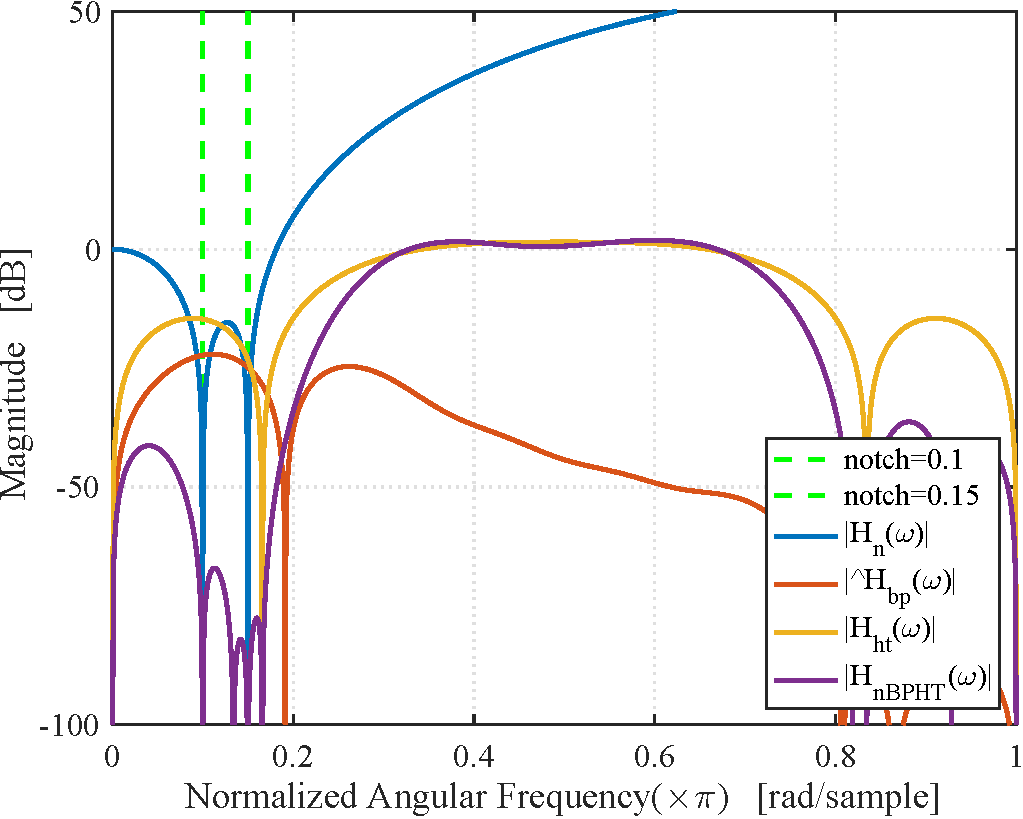
\includegraphics[width=8cm]
    		{Figure/figure01.pdf}
    \caption{のっちだおおおおおおお}
    \label{fig:man}
\end{figure}     <--第4章 まとめ
%#!platex main.tex
\chapter*{謝辞}
\addcontentsline{toc}{chapter}{謝辞} 
Other/thanks.texで文章を編集して下さい
%本研究にあたり,多大なるご指導とご助
%言を賜わりました.伊丹~ 誠教授,大野~光平先生に深く感謝いたします.また,色々
%な面でご協力いただいた伊丹研究室の大学院生の皆様,卒業研究生に対しまして
%も,心より感謝致します.最後に感謝の意を表して,本論文の謝辞とさせて頂きま
%す.

              <--謝辞
%#!platex main.tex
\chapter*{発表論文}
\addcontentsline{toc}{chapter}{発表論文}
\def\essection#1{\section*{#1}\addcontentsline{toc}{section}{#1}}

\essection{A.査読あり論文}
\begin{itemize}
\item Other/publicationで編集して下さい
\end{itemize}


\essection{B.国際会議}

\essection{C.研究会}

\essection{D.大会}

         <--発表論文リスト
\include{Other/bibliography}        <--参考文献
\end{verbatim}
です.
\begin{verbatim}
%#!platex main.tex
\chapter*{発表論文}
\addcontentsline{toc}{chapter}{発表論文}
\def\essection#1{\section*{#1}\addcontentsline{toc}{section}{#1}}

\essection{A.査読あり論文}
\begin{itemize}
\item Other/publicationで編集して下さい
\end{itemize}


\essection{B.国際会議}

\essection{C.研究会}

\essection{D.大会}


\end{verbatim}
は発表論文リストファイルですので卒論の場合,\verb|%|でコメントアウトして
 おいてください.

コンパイルの方法は

\framebox{\tt jlatex main.tex}

です.
しかし,これだけだと,目次が構成できないので,もう一度

\framebox{\tt jlatex main.tex}

とやると,目次も構成されます.
ちなみに,

\framebox{\tt make;make final}

とすると,main.psまではきます.
最後の最後の提出の時まではあまり使わないと思います.
修論などで,100ページ以上になると,psファイルがかなりでかくなるので,
 quotaに気をつけてください.
あと

\framebox{\tt make clean}

とすると,ディレクトリ内の掃除ができるのたまにやってもいいかも知れません.

また,yatexを利用すると,圧倒的に効率が良くなります.
この時,各LaTeXファイルに
\begin{verbatim}
%#!jlatex main.tex	
\end{verbatim}
という一行を加えておくと,どのLaTeXファイルからでもmain.texが呼べるので,
現在作業中のLaTeXファイル上で,jlatex main.texができます.
これはかなり便利です.
\section{おまけ}
図や表の引用で\verb|\ref|を利用すると思いますが,このスタイルでは
\verb|\ref{ラベル名}|とすると自動的に{\gt 図 {\bf 1}}のように出力するよ
うになっています.
これは表の引用,本文の引用においても同様です.
これが嫌な人はitlbthesis2012.styの最後の
\begin{verbatim}
\def\p@chapter{{\dg 本文}}
\def\p@section{{\dg 本文}}
\def\p@subsection{{\dg 本文}}
\def\p@subsubsection{{\dg 本文}}
\def\p@figure{{\dg 図}}
\def\p@table{{\dg 表}}
\let\origref=\ref
\def\ref#1{{\bf \origref{#1}}}
\end{verbatim}
を削除してください.


   <--第2章 スタイルファイルの使い方
\include{Figure/figure}             <--第3章 絵の貼り方
%#!platex main.tex
\chapter{序論}

\section{章タイトル}
参考文献のテスト\cite{樋口龍雄2000}.
"bibliography.bib"の中身をいじると変更できます.

あいうえおかきくけこ
正弦波の周波数推定はレーダーやソナー,通信,医療などの領域で幅広く研究されてきた課題である\cite{R.G.McKilliam,K.Wang,D.Rife}.
一般に,単一正弦波に対する周波数推定を行う場合,アナログ信号であれば周波数カウンタを用いる手法,ディジタル信号の場合,相関を用いた手法やヒルベルト変換器を用いる手法が提案されている.
周波数カウンタを用いた手法では,1周期に対して基準クロックを用いて測定し,その逆数から周波数を求めるレシプロカル方式の周波数カウンタが知られている.しかしこの手法を用いる場合,周波数が変化すると出力間隔が不等間隔になる.そのため,計測値に対して,ディジタル処理を行う場合には補完処理などの工夫が必要となるため,サンプルごとに周波数の推定値が出力されるヒルベルト変換器を用いた手法が提案されている.\\
 ヒルベルト変換器を用いた手法では,入力を実部,出力を虚部とする複素信号の一種である解析信号の位相を時間微分し,瞬時角周波数から瞬時周波数を推定することができる.従来,ヒルベルト変換器は有限次数のFIRフィルタとして設計されるため振幅特性にリプルが生じ,出力は振動する場合がある.高尾ら\cite{高尾可変なし,高尾可変あり}は振動成分の周波数が入力周波数の偶数倍であることを理論的に示し,これを伝送零点を有する可変FIRフィルタを用いて振動成分を除去することで,低次数なヒルベルト変換器を用いても,単一正弦波の高精度な瞬時周波数推定が可能となることを示した.
%高尾さんのやつと関連させてノイズを取れることを書きたいなら,どういうノイズが取れて,どういうノイズがダメなのか明記する必要がある.
しかし実際にはノイズを含む信号を解析する必要がある.一般に,ノイズを含む信号に対して,ヒルベルト変換を行うためには,あらかじめ帯域通過フィルタによりノイズを低減させた後に,ヒルベルト変換器を縦続接続する方法が考えられる.しかし,帯域通過フィルタとヒルベルト変換器を1つのフィルタとして見た場合,全体の次数が増加し,結果として遅延や回路規模の増大につながり好ましくない.\\
 そこで本稿では,阻止域を有するヒルベルト変換器に対し,指定した位置に伝送零点を置くことで,ノイズを除去しながらヒルベルト変換可能なフィルタを設計する.阻止域を有するヒルベルト変換器を設計する場合,本来であれば阻止域において十分な減衰量を確保するために多くのフィルタ次数が必要となる.しかし,特定の周波数成分にノイズが含まれることがわかっている場合,その周波数成分のみに伝送零点を入れることにより,特定のノイズのみ除去しながらヒルベルト変換を行うことができ,減衰量を確保するために必要な次数を削減することができる.
最後に設計例を示し,提案法の有効性を確認する.
\section{指定した位置に伝送零点を有するヒルベルト変換器}
本章では提案するフィルタの設計問題について記す.提案するフィルタは,阻止域の指定した位置に伝送零点を有するヒルベルト変換器である.本稿で設計するフィルタの振幅理想特性を図\ref{ideal_resp}に示す.またフィルタの振幅理想特性は正規化角周波数$\omega$を用いて,

\begin{figure}[tb]
    \centering
    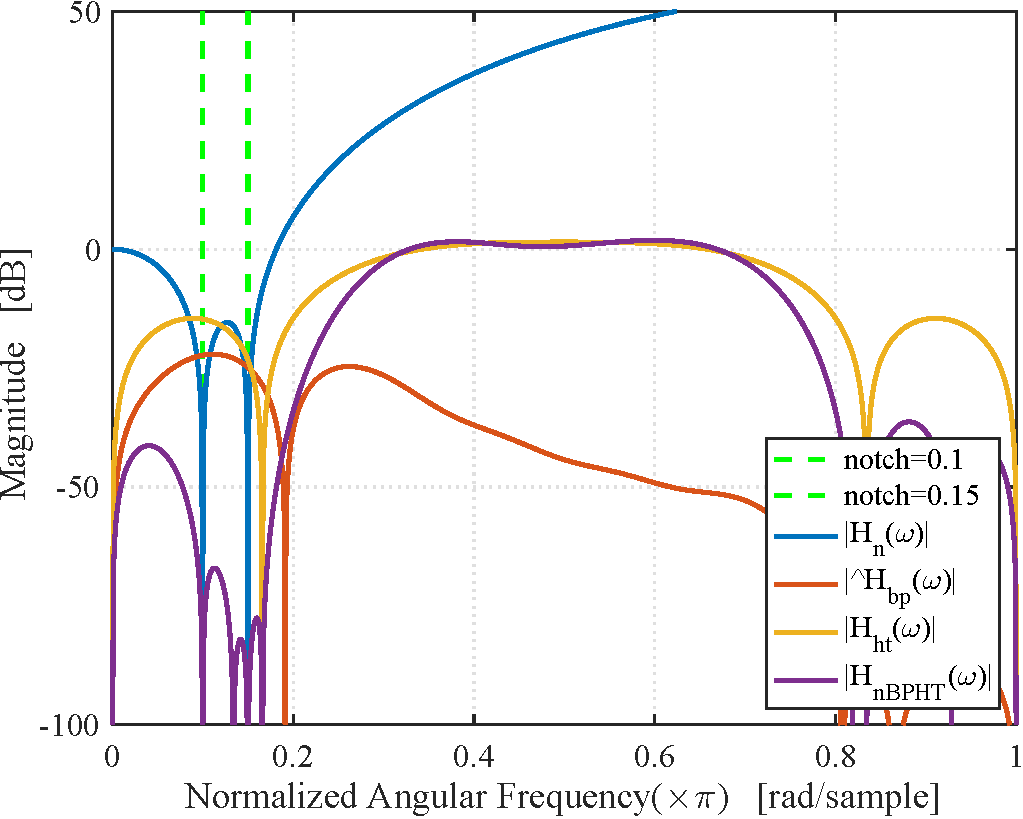
\includegraphics[width=8cm]
    		{Figure/figure01.pdf}
    \caption{のっちだおおおおおおお}
    \label{fig:man}
\end{figure}     <--第4章 まとめ
%#!platex main.tex
\chapter*{謝辞}
\addcontentsline{toc}{chapter}{謝辞} 
Other/thanks.texで文章を編集して下さい
%本研究にあたり,多大なるご指導とご助
%言を賜わりました.伊丹~ 誠教授,大野~光平先生に深く感謝いたします.また,色々
%な面でご協力いただいた伊丹研究室の大学院生の皆様,卒業研究生に対しまして
%も,心より感謝致します.最後に感謝の意を表して,本論文の謝辞とさせて頂きま
%す.

              <--謝辞
%#!platex main.tex
\chapter*{発表論文}
\addcontentsline{toc}{chapter}{発表論文}
\def\essection#1{\section*{#1}\addcontentsline{toc}{section}{#1}}

\essection{A.査読あり論文}
\begin{itemize}
\item Other/publicationで編集して下さい
\end{itemize}


\essection{B.国際会議}

\essection{C.研究会}

\essection{D.大会}

         <--発表論文リスト
\include{Other/bibliography}        <--参考文献
\end{verbatim}
です.
\begin{verbatim}
%#!platex main.tex
\chapter*{発表論文}
\addcontentsline{toc}{chapter}{発表論文}
\def\essection#1{\section*{#1}\addcontentsline{toc}{section}{#1}}

\essection{A.査読あり論文}
\begin{itemize}
\item Other/publicationで編集して下さい
\end{itemize}


\essection{B.国際会議}

\essection{C.研究会}

\essection{D.大会}


\end{verbatim}
は発表論文リストファイルですので卒論の場合,\verb|%|でコメントアウトして
 おいてください.

コンパイルの方法は

\framebox{\tt jlatex main.tex}

です.
しかし,これだけだと,目次が構成できないので,もう一度

\framebox{\tt jlatex main.tex}

とやると,目次も構成されます.
ちなみに,

\framebox{\tt make;make final}

とすると,main.psまではきます.
最後の最後の提出の時まではあまり使わないと思います.
修論などで,100ページ以上になると,psファイルがかなりでかくなるので,
 quotaに気をつけてください.
あと

\framebox{\tt make clean}

とすると,ディレクトリ内の掃除ができるのたまにやってもいいかも知れません.

また,yatexを利用すると,圧倒的に効率が良くなります.
この時,各LaTeXファイルに
\begin{verbatim}
%#!jlatex main.tex	
\end{verbatim}
という一行を加えておくと,どのLaTeXファイルからでもmain.texが呼べるので,
現在作業中のLaTeXファイル上で,jlatex main.texができます.
これはかなり便利です.
\section{おまけ}
図や表の引用で\verb|\ref|を利用すると思いますが,このスタイルでは
\verb|\ref{ラベル名}|とすると自動的に{\gt 図 {\bf 1}}のように出力するよ
うになっています.
これは表の引用,本文の引用においても同様です.
これが嫌な人はitlbthesis2012.styの最後の
\begin{verbatim}
\def\p@chapter{{\dg 本文}}
\def\p@section{{\dg 本文}}
\def\p@subsection{{\dg 本文}}
\def\p@subsubsection{{\dg 本文}}
\def\p@figure{{\dg 図}}
\def\p@table{{\dg 表}}
\let\origref=\ref
\def\ref#1{{\bf \origref{#1}}}
\end{verbatim}
を削除してください.


